\documentclass[12pt,a4paper,twoside,openright]{report}
\let\openright=\cleardoublepage



%%% Choose a language %%%

\newif\ifEN
\ENtrue   % uncomment this for english
%\ENfalse   % uncomment this for czech

%%% Configuration of the title page %%%

\newif\ifMFF
\MFFtrue % comment this out for the version with a big UK university logo
\def\UKName{Charles University in Prague} %this is only used in UK-logo-version
\def\UKFaculty{Faculty of Mathematics and Physics}

% Thesis type names, as used in several places in the title
%\def\ThesisTypeTitle{\ifEN BACHELOR THESIS \else BAKALÁŘSKÁ PRÁCE \fi}
\def\ThesisTypeTitle{\ifEN MASTER THESIS \else DIPLOMOVÁ PRÁCE \fi}
%\def\ThesisTypeTitle{\ifEN RIGOROUS THESIS \else RIGORÓZNÍ PRÁCE \fi}
%\def\ThesisTypeTitle{\ifEN DOCTORAL THESIS \else DISERTAČNÍ PRÁCE \fi}
%\%def\ThesisGenitive{\ifEN bachelor \else bakalářské \fi}
\def\ThesisGenitive{\ifEN master \else diplomové \fi}
%\def\ThesisGenitive{\ifEN rigorous \else rigorózní \fi}
%\def\ThesisGenitive{\ifEN doctoral \else disertační \fi}
%\def\ThesisAccusative{\ifEN bachelor \else bakalářskou \fi}
\def\ThesisAccusative{\ifEN master \else diplomovou \fi}
%\def\ThesisAccusative{\ifEN rigorous \else rigorózní \fi}
%\def\ThesisAccusative{\ifEN doctoral \else disertační \fi}



%%% Fill in your details %%%

% (Note: \xxx is a "ToDo label" which makes the unfilled visible. Remove it.)
\def\ThesisTitle{Prediction of velocity and speed of movement from human intracranial EEG recordings using deep neural networks}
\def\ThesisAuthor{Michaela Vystrčilová}
\def\YearSubmitted{2021}

% department assigned to the thesis
\def\Department{Department of Software and Computer Science Education}
% Is it a department (katedra), or an institute (ústav)?
\def\DeptType{Department}

\def\Supervisor{Mgr. Ján Antolík, PhD}
\def\SupervisorsDepartment{Department of Software and Computer Science Education}

% Study programme and specialization
\def\StudyProgramme{Computer Science}
\def\StudyBranch{IUI}

\def\Dedication{First, I would like to thank my supervisor Mgr. Ján Antolík, Ph.D. for introducing me to the intriguing field of neuroscience. His supportive attitude and advice helped me way beyond this thesis. In a similar manner I would like to thank Mgr. Jiří Hammer, Ph.D. who offered me not only this project but importantly also his time and knowledge. 

I also want to express my gratitude to Mr. Robin Tibor Schirrmeister, soon to be Ph.D. and professor Tonio Ball for their invaluable and welcoming consultations regarding the Deep4Net and brain signal processing in general.

Further I would like to manifest my appreciation for at least some of the people who, more or less directly, contributed to me starting and also finishing this thesis. For encouraging me not to content myself with something I would not enjoy doing, for standing me in times of quarantine and for all the emotional support and food, thank you, Vít Kabele, Jana, Jiří, Jana and Lenka Vystrčilovi, Anna Bláhová. 

Last, but not least, I would like to thank my cat for sitting on my lap long enough for me to be able to finish the thesis. 
}

\def\AbstractEN{%
Our brain controls the processes of the body including movement. In this thesis we try to understand, how the information about hand movement is encoded into the brain's electrical activity and how this activity can be used to predict the velocity and absolute velocity of hand movements. Using a well-established deep neural network architecture for EEG decoding - the Deep4Net - we predict hand movement velocity and absolute velocity from intracranial EEG signals. While reaching the expected performance level, we determine the influence of different frequency bands on the network's prediction. We find that modulations in the high-gamma frequency band are less informative than expected based on previous studies. We also identify two architectural modifications which lead to higher performances. 1. the removal of max-pooling layers in the architecture leads to significantly higher correlations. 2. the non-uniform receptive field of the network is a potential drawback making the network biased towards less relevant information. 
% ABSTRACT IS NOT A COPY OF YOUR THESIS ASSIGNMENT!
}

\def\AbstractCS{Lidský mozek řídí naše těla včetně pohybů rukou. V této diplomové práci jsme se snažili porozumět tomu, jak je informace o pohybu rukou zakódovaná do elektrické aktivity mozku a jak lze tuto aktivitu použít při predikování rychlosti a absolutní rychlosti pohybu rukou. Pomocí osvědčené hluboké neuronové sítě (Deep4Net), používané k dekódování signálů z EEG, jsme dekódovali rychlost a absolutní rychlost pohybů rukou z intrakraniálního EEG. Úspěšnějsme dosáhli očekávaných hodnot korelace mezi predikovanými a skutečnými proměnnými. Zároveň jsme stanovili vliv amplitud vlnových pásem v různých frekveních na predikce této sítě. Zjistili jsme, že vliv modulací ve vlnovém pásmu high-gamma je menší než se očekávalo na základě předchozích studií. Současně jsme identifikovali dvě možné úpravy architektury Deep4Net, které mohou vést k lepším predikčním schopnostem.  Zaprvé jsme odhalili, že odstraněním max-poolingových vrstev lze dosáhnout statisticky signifikantně lepších korelačních koeficientů. Zadruhé jsme objevili, že nerovnoměrné receptivní pole této sítě představuje nevýhodu a způsobuje že se vícesoustřeďují na méně relevantní informace.}

% 3 to 5 keywords (recommended), each enclosed in curly braces.
% Keywords are useful for indexing and searching for the theses by topic.
\def\Keywords{%
{{motor decoding}, {intracranial EEG (iEEG)}, {deep learning}, {convolutional neural networks}}
}

% If your abstracts are long and do not fit in the infopage, you can make the
% fonts a bit smaller by this setting. (Also, you should try to compress your abstract more.)
% Alternatively, consider increasing the size of the page by uncommenting the
% geometry modification in thesis.tex.
\def\InfoPageFont{}
%\def\InfoPageFont{\small}  %uncomment to decrease font size

\ifEN\relax\else
% If you are writing a czech thesis, you additionally need to fill in the
% english translation of the metadata here!
\def\ThesisTitleEN{\xxx{Thesis title in English}}
\def\DepartmentEN{\xxx{Name of the department in English}}
\def\DeptTypeEN{\xxx{Department}}
\def\SupervisorsDepartmentEN{\xxx{Superdepartment}}
\def\StudyProgrammeEN{\xxx{study programme}}
\def\StudyBranchEN{\xxx{study branch}}
\def\KeywordsEN{%
\xxx{{key} {words}}
}
\fi


\usepackage[a-2u]{pdfx}

\ifEN\else\usepackage[czech,shorthands=off]{babel}\fi
\usepackage[utf8]{inputenc}
\usepackage[T1]{fontenc}

% See https://en.wikipedia.org/wiki/Canons_of_page_construction before
% modifying the size of printable area. LaTeX defaults are great.
% If you feel it would help anything, you can enlarge the printable area a bit:
%\usepackage[textwidth=390pt,textheight=630pt]{geometry}
% The official recommendation expands the area quite a bit (looks pretty harsh):
%\usepackage[textwidth=145mm,textheight=247mm]{geometry}

%%% FONTS %%%
\usepackage{lmodern} % TeX "original" (this sets up the latin mono)

% Optionally choose an override for the main font for typesetting
\usepackage[mono=false]{libertinus} % popular for comp-sci (ACM uses this)
%\usepackage{tgschola} % Schoolbook-like (gives a bit of historic feel)
%\usepackage[scale=0.96]{tgpagella} % Palladio-like (popular in formal logic).

% Optionally choose a custom sans-serif fonts (e.g. for figures and tables).
% Default sans-serif font is usually Latin Modern Sans. Some font packages
% (e.g. libertinus) replace that with a better matching sans-serif font.
%\usepackage{tgheros} % recommended and very readable (Helvetica-like)
%\usepackage{FiraSans} % looks great
% DO NOT typeset the main text in sans-serif font!
% The serifs make the text easily readable on the paper.

% IMPORTANT FONT NOTE: Some fonts require additional PDF/A conversion using
% the pdfa.sh script. These currently include only 'tgpagella'; but various
% other fonts from the texlive distribution need that too (mainly the Droid
% font family).


% some useful packages
\usepackage{amsmath,amsfonts,amsthm,bm}
\usepackage{graphicx}
\usepackage{xcolor}
\usepackage{booktabs}
\usepackage{floatrow}

% load bibliography tools
%\usepackage[backend=bibtex,natbib,style=numeric,sorting=none]{biblatex}
% alternative with alphanumeric citations (more informative than numbers):
\usepackage[backend=bibtex,natbib,style=authoryear,giveninits=true,maxnames=1]{biblatex}
%\usepackage[nottoc]{tocbibind}

%
% alternatives that conform to iso690
% (iso690 is not formally required on MFF, but may help elsewhere):
%\usepackage[backend=bibtex,natbib,style=iso-numeric,sorting=none]{biblatex}
%\usepackage[backend=bibtex,natbib,style=iso-alphabetic]{biblatex}
%
% additional option choices:
%  - add `giveninits=true` to typeset "E. A. Poe" instead of full Edgar Allan
%  - `terseinits=true` additionaly shortens it to nature-like "Poe EA"
%  - add `maxnames=10` to limit (or loosen) the maximum number of authors in
%    bibliography entry before shortening to `et al.` (useful when referring to
%    book collections that may have hundreds of authors)
%  - for additional flexibility (e.g. multiple reference sections, etc.),
%    remove `backend=bibtex` and compile with `biber` instead of `bibtex` (see
%    Makefile)
%  - `sorting=none` causes the bibliography list to be ordered by the order of
%    citation as they appear in the text, which is usually the desired behavior
%    with numeric citations. Additionally you can use a style like
%    `numeric-comp` that compresses the long lists of citations such as
%    [1,2,3,4,5,6,7,8] to simpler [1--8]. This is especially useful if you plan
%    to add tremendous amounts of citations, as usual in life sciences and
%    bioinformatics.
%  - if you don't like the "In:" appearing in the bibliography, use the
%    extended style (`ext-numeric` or `ext-alphabetic`), and add option
%    `articlein=false`.
%
% possibly reverse the names of the authors with the default styles:
%\DeclareNameAlias{default}{family-given}

% load the file with bibliography entries
\addbibresource{refs.bib}

% remove this if you won't use fancy verbatim environments
\usepackage{fancyvrb}

% remove this if you won't typeset TikZ graphics
\usepackage{tikz}
\usetikzlibrary{positioning} %add libraries as needed (shapes, decorations, ...)

% remove this if you won't typeset any pseudocode
\usepackage{algpseudocode}
\usepackage{algorithm}
% remove this if you won't list any source code
\usepackage{listings}
\usepackage{subcaption}
\usepackage{mathabx}


\hypersetup{unicode}
\hypersetup{breaklinks=true}

\usepackage[noabbrev]{cleveref}
\usepackage{algorithmicx}
\usepackage{lipsum}


% various forms of TODOs (you should remove this before submitting)
\usepackage[textsize=tiny, backgroundcolor=yellow!25, linecolor=black!25]{todonotes}
\newcommand{\xxx}[1]{\textcolor{red!}{#1}}

 % remove this before compiling the final version


% use this for typesetting a chapter without a number, e.g. intro and outro
\def\chapwithtoc#1{
\chapter*{#1}
\addcontentsline{toc}{chapter}{#1}
}

% If there is a line/figure overflowing into page margin, this will make the
% problem evident by drawing a thick black line at the overflowing spot. You
% should not disable this.
\overfullrule=3mm

% The maximum stretching of a space. Increasing this makes the text a bit more
% sloppy, but may prevent the overflows by moving words to next line.
\emergencystretch=1em

\ifEN
\theoremstyle{plain}
\newtheorem{thm}{Theorem}
\newtheorem{lemma}[thm]{Lemma}
\newtheorem{claim}[thm]{Claim}
\newtheorem{defn}{Definition}
\theoremstyle{remark}
\newtheorem*{cor}{Corollary}
\else
\theoremstyle{plain}
\newtheorem{thm}{Věta}
\newtheorem{lemma}{Lemma}
\newtheorem{claim}{Tvrzení}
\newtheorem{defn}{Definice}
\theoremstyle{remark}
\newtheorem*{cor}{Důsledek}
\fi

\newenvironment{myproof}{
  \par\medskip\noindent
  \textit{\ifEN Proof \else Důkaz \fi}.
}{
\newline
\rightline{$\qedsymbol$}
}

% real/natural numbers
\newcommand{\R}{\mathbb{R}}
\newcommand{\N}{\mathbb{N}}

% asymptotic complexity
\newcommand{\asy}[1]{\mathcal{O}(#1)}

% listings and default lstlisting config (remove if unused)
\DeclareNewFloatType{listing}{}
\floatsetup[listing]{style=ruled}

\DeclareCaptionStyle{thesis}{style=base,font={small,sf},labelfont=bf,labelsep=quad}
\captionsetup{style=thesis}
\captionsetup[algorithm]{style=thesis,singlelinecheck=off}
\captionsetup[listing]{style=thesis,singlelinecheck=off}

\ifEN\floatname{listing}{Listing}
\else\floatname{listing}{Výpis kódu}\fi
\lstset{%
  language=C++,
  tabsize=2,
  showstringspaces=false,
  basicstyle=\footnotesize\tt\color{black!75},
  identifierstyle=\bfseries\color{black},
  commentstyle=\color{green!50!black},
  stringstyle=\color{red!50!black},
  keywordstyle=\color{blue!75!black}}

% Czech versions of the used cleveref references (It's not as convenient as in
% English because of declension, cleveref is limited to sg/pl nominative. Use
% plain \ref to dodge that.)
\ifEN\relax\else
\crefname{chapter}{kapitola}{kapitoly}
\Crefname{chapter}{Kapitola}{Kapitoly}
\crefname{section}{sekce}{sekce}
\Crefname{section}{Sekce}{Sekce}
\crefname{subsection}{sekce}{sekce}
\Crefname{subsection}{Sekce}{Sekce}
\crefname{subsubsection}{sekce}{sekce}
\Crefname{subsubsection}{Sekce}{Sekce}
\crefname{figure}{obrázek}{obrázky}
\Crefname{figure}{Obrázek}{Obrázky}
\crefname{table}{tabulka}{tabulky}
\Crefname{table}{Tabulka}{Tabulky}
\crefname{listing}{výpis}{výpisy}
\Crefname{listing}{Výpis}{Výpisy}
\floatname{algorithm}{Algoritmus}
\crefname{algorithm}{algoritmus}{algoritmy}
\Crefname{algorithm}{Algoritmus}{Algoritmy}
\newcommand{\crefpairconjunction}{ a~}
\newcommand{\crefrangeconjunction}{ a~}
\fi
 % use this file for various custom definitions


\begin{document}

% the layout is mandatory, edit only in dire circumstances

\pagestyle{empty}
\hypersetup{pageanchor=false}
\begin{center}

\ifMFF
\ifEN
\centerline{\mbox{
\includegraphics[width=166mm]{img/logo-en.pdf}}}
\else
\centerline{\mbox{
\includegraphics[width=166mm]{img/logo-cs.pdf}}}
\fi
\vspace{-8mm}
\else
{\large\noindent\UKName\par\medskip\par\UKFaculty }
\fi
\vfill

{\bf\Large\ThesisTypeTitle}

\vfill

\ifMFF\relax\else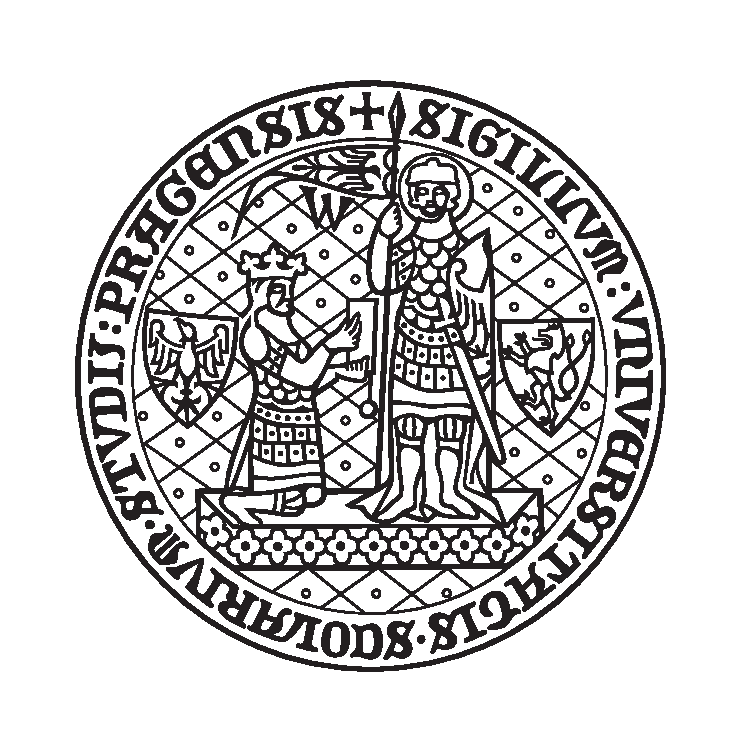
\includegraphics[width=70mm]{img/uklogo.pdf}

\vfill\fi

{\LARGE\ThesisAuthor}

\vspace{15mm}

{\LARGE\bfseries\ThesisTitle}

\vfill

\Department

\vfill

{
\centerline{\vbox{\halign{\hbox to 0.45\hsize{\hfil #}&\hskip 0.5em\parbox[t]{0.45\hsize}{\raggedright #}\cr
\ifEN Supervisor of the \ThesisGenitive thesis:
\else Vedoucí \ThesisGenitive práce: \fi
& \Supervisor \cr
\noalign{\vspace{2mm}}
\ifEN Study programme: \else Studijní program: \fi
& \StudyProgramme \cr
\noalign{\vspace{2mm}}
\ifEN Study branch: \else Studijní obor: \fi
& \StudyBranch \cr
}}}}

\vfill

\ifEN Prague \else Praha \fi
\YearSubmitted

\end{center}

\newpage

% remember to sign this!
\openright
\hypersetup{pageanchor=true}
\pagestyle{plain}
\pagenumbering{roman}
\vglue 0pt plus 1fill

\ifEN
\noindent
I declare that I carried out this \ThesisAccusative thesis independently, and only with the cited
sources, literature and other professional sources. It has not been used to obtain another
or the same degree.
\else
\noindent
Prohlašuji, že jsem tuto \ThesisAccusative práci vypracoval(a) samostatně a výhradně
s~použitím citovaných pramenů, literatury a dalších odborných zdrojů.
Tato práce nebyla využita k získání jiného nebo stejného titulu.
\fi

\ifEN
\medskip\noindent
I understand that my work relates to the rights and obligations under the Act No.~121/2000 Sb.,
the Copyright Act, as amended, in particular the fact that the Charles
University has the right to conclude a license agreement on the use of this
work as a school work pursuant to Section 60 subsection 1 of the Copyright~Act.
\else
\medskip\noindent
Beru na~vědomí, že se na moji práci vztahují práva a povinnosti vyplývající
ze zákona č. 121/2000 Sb., autorského zákona v~platném znění, zejména skutečnost,
že Univerzita Karlova má právo na~uzavření licenční smlouvy o~užití této
práce jako školního díla podle §60 odst. 1 autorského zákona.
\fi

\vspace{10mm}


\ifEN
\hbox{\hbox to 0.5\hsize{%
In \hbox to 6em{\dotfill} date \hbox to 6em{\dotfill}
\hss}\hbox to 0.5\hsize{\dotfill\quad}}
\smallskip
\hbox{\hbox to 0.5\hsize{}\hbox to 0.5\hsize{\hfil Author's signature\hfil}}
\else
\hbox{\hbox to 0.5\hsize{%
V \hbox to 6em{\dotfill} dne \hbox to 6em{\dotfill}
\hss}\hbox to 0.5\hsize{\dotfill\quad}}
\smallskip
\hbox{\hbox to 0.5\hsize{}\hbox to 0.5\hsize{\hfil Podpis autora\hfil}}
\fi

\vspace{20mm}
\newpage

% dedication

\openright

\noindent
\Dedication

\newpage

% mandatory information page

\openright

\vbox to 0.49\vsize{\InfoPageFont
\setlength\parindent{0mm}
\setlength\parskip{5mm}

\ifEN Title: \else Název práce: \fi
\ThesisTitle

\ifEN Author: \else Autor: \fi
\ThesisAuthor

\DeptType:
\Department

\ifEN Supervisor: \else Vedoucí bakalářské práce: \fi
\Supervisor, \SupervisorsDepartment

\ifEN Abstract: \AbstractEN \else Abstrakt: \AbstractCS \fi

\ifEN Keywords: \else Klíčová slova: \fi
\Keywords

\vss}\ifEN\relax\else\nobreak\vbox to 0.49\vsize{\InfoPageFont
\setlength\parindent{0mm}
\setlength\parskip{5mm}

Title:
\ThesisTitleEN

Author:
\ThesisAuthor

\DeptTypeEN:
\DepartmentEN

Supervisor:
\Supervisor, \SupervisorsDepartmentEN

Abstract:
\AbstractEN

Keywords:
\KeywordsEN

\vss}
\fi

\newpage

\openright
\pagestyle{plain}
\pagenumbering{arabic}
\setcounter{page}{1}


\tableofcontents


\chapter{Introduction}
\label{chap:intr}

\section*{Historical context}
While mankind has been fascinated by the human mind for a long time, only the last 70 years of rapid technological advances finally allowed us to peer deep into the human brain.
New recording techniques, theoretical models, and detailed simulations facilitated by the increase in computational power have opened new horizons in the field of neuroscience.
But to this day, a lot remains unclear about how the activity of billions of neural cells interconnected through a dense web of dynamic circuits translates into complex processes such as perception, movement, reasoning or learning.  

One of the recent subfields of neuroscience, namely \textit{computational neuroscience}, combines neuroscience with mathematics and computer science to formulate theoretical principles governing the nervous system. 
The earliest theoretical discoveries in the field of neuroscience were models of single neurons (\cite{lapique-1907, hodgkin1952quantitative}).
Modeling activity of single neurons, however, cannot capture the brain in its whole complexity.
Because the billions of neurons and other neural cells are constantly communicating with each other, their coordinated activity is another key to unlocking the brain’s mysteries.
Methods capturing and interpreting such activity are therefore needed.
In 1924, Hans Berger was the first one to record human brain activity through electroencephalography (EEG).
Since then, many other recording techniques for measuring aggregate signal from large population of neurons emerged such as magnetoencephalography (MEG), functional magnetic resonance imaging (fMRI), positron emission tomography (PET), magnetic resonance spectroscopy (MRS), etc.  

There is a long path from recording brain activity to understanding how it translates into processes the brain governs in humans.
One approach to formulate a relationship between brain signal and a certain process such as movement or sleep is called \textit{brain signal decoding} or also \textit{neural decoding}.
It studies what information is available in the electrical activity of neurons or networks of neurons through mapping patterns in the electrical activity onto external processes such as movement or sleep.
To create such a mapping, first, brain signal is recorded simultaneously with a variable describing the process. 
Then a model predicting the variable based on the brain signal is built and fitted to the recorded data.
These models not only allow for a deeper understanding of the information contained in brain activity but have also direct clinical applications.
They are being used for predicting epileptic seizures (\cite{epileptic-seizures-eeg}), Alzheimer disease diagnosis (\cite{alzheimer-eeg}), classifying sleep stages (\cite{sleep-stage-alg-comparison}) or in Brain-computer interfacing (BCIs) (\cite{ecog-bci, eeg-bci}).

Artificial neural networks, which elevated what is considered state-of-the-art  in various fields, most prominently computer vision (\cite{dnn-computer-vision}) and natural language processing (\cite{dnn-nlp}), are being increasingly utilized as such models (\cite{Roy-2019}). 
Their ability to process complex data in and end-to-end manner together with good prediction performance makes them suitable for decoding from brain signals. 


\section*{Motivation}
Utilizing recent advances in deep learning (DL) in movement decoding from (EEG) has brought considerable progress in this field.
In multiple cases, deep neural networks have been shown to be more effective when decoding from EEG and intracranial EEG than standard machine learning methods (\cite{Zhang-2019, lawhern-eegnet-2018, sleep-eegnet}).
Nevertheless, there is still room for considerable improvement in the decoding accuracy, interpretability and applicability to online decoding (\cite{Roy-2019}). 
These issues are even more substantial in movement decoding from intracranial EEG (iEEG). 
Because it is more difficult to acquire iEEG data, it is less researched but very promising because of the higher signal-to-noise ration of iEEG signal compared to EEG (\cite{volkova-review}). 

To address these issues, \cite{Hammer-2021} employed the Deep4Net - a convolutional neural network introduced in \cite{schirrmeister-deep-2017} - to perform iEEG movement decoding, namely to decode hand velocity and absolute velocity (speed) from intracranial EEG. 
The Deep4Net was chosen because in previous studies (\cite{schirrmeister-deep-2017, hartmann-hierarchical-2018}) it has proven successful in movement-related classification tasks, reaching comparable accuracy with state-of-the-art methods without the necessity of manual feature extraction.
When using it, \cite{schirrmeister-deep-2017} also inspected the which frequency bands are important for the network's decisions. Besides confirming the informativeness of the alpha and beta bands, it was the first time that the importance of modulations in the high-gamma band was shown for movement decoding from non-invasive EEG.
The fact that Deep4Net architecture is able to extract information from the high-gamma band suggests its suitability for iEEG decoding, where the high frequency resolution is better than in non-invasive EEG (\cite{gamma-eeg-bad-resolution}). 

\cite{Hammer-2021} found that the Deep4Net significantly outperforms multi-linear regression in velocity and absolute velocity decoding.
Nevertheless, when visualizing which features it focuses on, the network has not shown the expected interest in the high-gamma frequency modulations. 
In the context of previous findings on the same dataset, where high-gamma was found significant, especially for absolute velocity decoding when using multi-linear regression (\cite{hammer-predominance-2016}) and the fact that the Deep4Net architecture is able to extract information from the high-gamma frequency (\cite{schirrmeister-deep-2017}), the group briefly continued to explore this surprising finding.

Using a different visualization method, namely gradient visualization, they discovered a gradient peak in the high-gamma range at 83.33~Hz showing possible interest of the network in information from the high-gamma frequency (personal communication).
Multiple questions remain to be answered at this point: Is the gradient peak significant or is it just an architecture artifact?
If it is an architecture artifact, why did the network not use the high-gamma?
Would other architectures be able to utilize high-gamma in this setting?
Could we improve performance by forcing the network to use high-gamma?
Is high-gamma indeed informative for (absolute) velocity of movement decoding? 
If the peak is not an architecture artifact but reflects the use of information from the high-gamma band by the network, why did the perturbation visualization method performed by \cite{Hammer-2021} not show it?\\
\\


\section*{Goals}
The aim of this thesis is to address the above outlined questions which can be summarized in the two following goals:

\begin{enumerate}
    \item Understanding which frequency bands are utilized by the Deep4Net in \cite{Hammer-2021} for hand movement decoding with particular focus on the high-gamma band 
    \item Identifying which modifications to DNN training/architecture improve the utilization of information across useful frequency bands.
\end{enumerate}

Achieving these goals will contribute to the interpretability of deep neural networks used for iEEG movement decoding.
By identifying informative frequency bands and optimizing the network architecture to use them effectively, we can also potentially improve the decoding performance of these networks, advancing their clinical application.


%\chapter{Introduction}
\label{chap:intr}

F 
\chapter{Background and related work}
\label{chap:background}
In this chapter, we give a brief introduction of topics most relevant for this thesis to equip the reader with the necessary background.
We start by shortly describing (intracranial) EEG signals, their standard feature extraction and decoding techniques (Section \ref{sec:decoding-from-ieeg}). We further provide a concise introduction to deep neural networks (DNNs) paying special attention to convolutional neural networks (CNNs) (Section \ref{sec:artificial-neural-networks}).
Lastly, we introduce the two most relevant papers (\cite{Hammer-2021}) and (\cite{schirrmeister-deep-2017}) in more detail, followed by brief descriptions of other DNN architectures used for movement decoding (Section \ref{sec:dnn-decoding}).

\section{Decoding from (i)EEG signals}
\label{sec:decoding-from-ieeg}
Neural decoding refers to a neuroscience field concerned with the reconstruction of external stimuli from information that is already encoded in the brain. 
It consists of multiple stages, namely, signal recording, spectral and spatial feature extraction and the final classification or regression algorithm. 
In this section, we describe the methods traditionally used in each of these stages highlighting their advantages and disadvantages. 
While many things, such as sleep stages (\cite{sleep-eegnet}), epileptic seizures (\cite{epileptic-seizures-eeg}) or emotions (\cite{emotion-eeg}) can be decoded from brain signals, we introduce mainly methods used for movement decoding because they are most relevant for this thesis. 

\subsection{Recording methods}
An existing correlation between neural modulations and motor parameters for a wide range of motor tasks makes electrical brain activity suitable for movement decoding  (\cite{lebedev-cortical-2005}).
Electroencephalography (EEG), electrocorticography (ECoG) and stereo-tactic EEG (sEEG) are the most commonly used techniques of recording electrical activity of the brain (\cite{tam-human-2019}).
We describe basic properties of each of these recording methods. For a more detailed introduction to EEG please refer to \cite{NiedermeyersElectroencephalography}.

\subsubsection{Electroencephalography (EEG)}
Electroencephalography (EEG) records electrical brain activity of the cerebral cortex using multiple electrodes (also called channels) which are placed on the surface of the head. The recorded activity, originating as the postsynaptic potential of excitable neural tissue (\cite{buzsaki-origin-2012}), is attenuated through cerebrospinal fluid, the dura and the skull on its way to the recording electrodes. Besides weakening the signal, these structures also act as low-pass filters limiting the useful frequency bands to below 100~Hz (\cite{tam-human-2019}). Another limitation of EEG recordings is the interference of activity of muscles located in the region of the head. Muscle activity has higher amplitudes than brain signals and can therefore affect the recording quality (\cite{scholg-presence-2002}). It lowers the signal to noise ratio of EEG signals. EEG has also relatively poor spatial resolution (\cite{buzsaki-origin-2012}). Despite the aforementioned drawbacks, EEG is a widely used tool in brain signal recording. Its high temporal resolution, safety and a relatively low cost motivate researchers to develop new quality control and artifact processing techniques (\cite{lotte2018review}) to alleviate the disadvantages of EEG. 

\subsubsection{Electrocorticography and stereo-tactic EEG}
Electrocorticography (ECoG) and stereo-tactic electroencephalography (sEEG) are variations of EEG commonly referred to as intracranial EEG (iEEG).
In ECoG, a grid with multiple recording electrodes (channels) is placed on the surface of the brain instead of the surface of the head.
For stereo-tactic EEG, the electrodes penetrate the skull and reach deeper inside the brain. Both are very invasive methods and cannot be performed for the sake of research only.
Therefore, intracranial EEG studies are mainly conducted on patients with medication resistant epilepsy.
The electrodes are used to find the locus of seizures which is then surgically removed. When Special measures have to be taken to remove channels displaying pathological symptoms when using ECoG signal for research.
The quality of signal from non-epileptic brain tissue is, however, superior to standard EEG. It has higher spatial resolution as well as better resolution in the high frequencies (\cite{volkova-review}).

\subsection{Feature extraction}
End-to-end learning has started to be used only recently and manual feature extraction is still common when designing movement decoders from EEG and iEEG.
We will describe some widely used feature extraction methods. 
Often distinct methods are used for spatial and temporal information both of which are present in EEG and iEEG signals. 
Spatial information tells us where in or on the brain the signal was measured depending on the position of the electrode.
Temporal information contains information about when the signal was recorded and what its value was in that moment.
\subsubsection{Spatial feature extraction}
Spatial feature extraction methods are used for signal denoising, rejection of pathological channels and dimensionality reduction.
 Common average reference (CAR) is a widely used and simple denoising method.
 In CAR, the mean of all channels is subtracted from each channel (\cite{liu-effects-2015}).
 This reduces noise common to all channels but might introduce some channel specific noise to some otherwise clean channels (\cite{volkova-review}). 
 Multiple other methods have been proposed to address this issue.
 For example auto-regressive models which instead of subtracting the mean of the channels assign a weight to each channel, so that it minimizes the variance, and then subtract this weighted average from each channel (\cite{adaptive-laplacian-reference}).
 Bipolar reference and Laplacian reference (\cite{yao2019reference, laplacian-reference}) are also ways to avoid proposing channel specific noise by focusing only on the re-referencing of neighbouring channels.
 
 
Noisy and epileptic channel rejection is often done after visual inspection by experts. Nevertheless, automatic mechanisms to select channels for removal have also been developed. A noisy channel can be identified based on an abnormal distribution, identification of excessive line noise or the outliers it contains (\cite{liu-effects-2015}). If a channel is marked noisy, it is removed from the dataset. However, some studies propose the use of CAR with median subtraction instead of mean subtraction while keeping all channels. They claim that this way it is possible to retain all information potentially valuable for decoding while also sufficiently reducing noise across all channels (\cite{liu-effects-2015}). 

Recording from multiple electrodes creates highly dimensional data. Reducing their complexity is another opportunity for spatial feature extraction to help achieve better decoding results. Principal component analysis (PCA) (\cite{pca}) is a commonly used method (\cite{volkova-review}). It transforms the data into a new coordinate system achieving largest possible variance along the axes. Optionally, one can then discard the axes with lower variance to achieve dimensionality reduction. Independent component analysis, another tool for dimensionality reduction, also transforms the data into a new coordinate system. 
But unlike PCA, it selects a basis in which each vector is an independent component of the data (\cite{ica}).

\subsubsection{Spectral feature extraction}
Spectral feature extraction methods are used to extract task-related features from the time-domain and power spectra domain. Regarding the time-domain, the Low-pass filtered component (LFC), also called Local motor potential (LMP) which can be extracted using Savitzky-Golay filters (\cite{multitaper-31}) has been shown by multiple studies to hold information about movement time-course and kinematics (\cite{schalk-2007, Pistohl2008PredictionOA, ball-2019}). 

In the power spectrum domain, following are the traditionally defined frequency ranges: $\delta$~(0–4~Hz), $\theta$ (4–8~Hz), $\alpha$ (8–12~Hz), $\beta$ (13–30~Hz), low $\gamma$ (30–70~Hz) and in the case of ECoG high $\gamma$ band (70~Hz and above) (\cite{hammer-predominance-2016}). The modulations in the alpha, beta and in the case of intracranial EEG also high-gamma bands are particularly informative for movement decoding (\cite{ball-hg-importance, 34-gunduz-hg}). As previously stated, the high-gamma signal from EEG is often noisy and not suitable for decoding. However, it has been recently shown that neural networks are able to use information from the high-gamma band for movement classification (\cite{schirrmeister-deep-2017}).

Multiple methods have been proposed to extract features from the power spectrum domain.
The signal can be either directly band-filtered in the desired range or converted into the frequency domain using both non-parametric and parametric methods.
Non-parametric methods include Fourier analysis, multi-taper methods and wavelet transformations (\cite{volkova-review}).

Fourier analysis involves convolving the brain signal with a sinusoidal function of a fixed length. The analysis is performed on short windows to improve temporal specificity, nevertheless, its time-frequency resolution is quite poor.
Moreover, it is only useful in a limited frequency range, based on the window size and the size fixes also the scale of the signal that is to be detected (\cite{36-vugt-2007}). 
Both multi-tapering methods and wavelets were designed to ameliorate these issues. 

Decomposing the signals into shifted and scaled versions of an oscillating waveform of a wavelet function allows the proportion between the temporal width and frequency band-with to stay the same for all frequencies. 
This contributes to a higher temporal resolution in higher frequencies. The good time-frequency trade-off of wavelets makes them suitable for analysing non-stationary signals (\cite{36-vugt-2007}).  

Multi-taper methods were designed to reduce bleeding between frequencies making them, too, well-suited for analyzing signals of non-stationary processes. 
Tapers are functions having a value of one in the middle and then taper to zero at the edges. 
The multi in multi-taper implies that the signal is convolved with multiple such orthogonal tapers.
These are then averaged yielding a statistically consistent spectral estimator with reduced variance of the spectral estimates and improved localisation in the frequency domain (\cite{multitaper-31}).

Auto-regressive spectral estimators (AR) are parametric spectral feature extractors.
They have proven successful for modelling both EEG (\cite{auto-regressive-eeg}) and iEEG (\cite{anderson-offline-2009}).
Even though ARs have an inherent capacity to model peaky spectra characteristic for bio-signal, their effectivity largely depends on parameterization, which is not particularly straight-forward (\cite{anderson-offline-2009}). 

More recently proposed approaches based on Riemann geometry which use covariance matrices to for feature learning and representation have shown promising results (\cite{coherence-based}).
Temporal modulations can also be modeled probabilistically using hidden Markov's models or conditional random fields (\cite{markov-models-decoding, bayesian-decoding}).
Importantly, also neural networks can be integrated in the movement decoding pipeline as feature extractors.
For example auto-encoders are suited for dimensionality reduction \cite{autoencoder}.
An auto-encoder consists of two parts.
The encoder first compresses the data into a smaller representation.
The decoder then receives the compressed data and without information about their initial form tries to reconstruct them.
This forces the encoder to create a smaller representation which, however, contains as much information as possible.
Convolutional neural networks are also particularly useful in signal processing because many of the aforementioned filters can be implemented as convolutions. 


\subsection{Classification methods}
Various movement related classification tasks such as decoding wrist flexion or extension (\cite{wrist-flexion}) movement of individual fingers (\cite{cond-rf-finger-class, lda-finger-movement-classification}) or feet movement (\cite{feet-movement}) from EEG and iEEG have been studied using a diverse population of classifiers.  
The classifiers include Support vector machines (SVM) (\cite{svm-alg}), Linear Discriminant analysis (LDA) (\cite{lda-paper}), Quadratic discriminant analysis (QDA) (\cite{qda-paper}), their adaptive versions which have gained popularity in the last ten years (\cite{lotte2018review}) and probabilistic methods such as conditional random fields or naive bayes classifiers (\cite{bayesian-decoding, cond-rf-finger-class}). 


\subsection{Regression methods}
Regression tasks attracted less attention from researchers than classification tasks (\cite{volkova-review}).
Still, extensive research with many different kinds of tasks was conducted on this front as well.
Movement decoding tasks which fall in the category of regression include finger position decoding (\cite{Pistohl2008PredictionOA}), hand position decoding (\cite{ball-2019}) or
kinematic variables such as speed or velocity decoding of hand movements (\cite{hammer-role-2013, hammer-predominance-2016, Hammer-2021, kalman-filters-velocity, linear-regression-eeg-hand-3d}).
Various algorithms have been employed to solve the above listed tasks. 
Models based on linear regression combined with various feature extraction methods are very common (\cite{hammer-role-2013, hammer-predominance-2016, eeg-hand-moving, linear-regression-eeg-hand-3d}).
More sophisticated models include Kalman filters (\cite{kalman-filters-velocity}) and their unscented versions (\cite{uns-kalman-filters-gait-decoding}).
Neural networks which we describe separately in Section~\ref{sec:dnn-decoding} have also been proposed to solve movement related regression tasks.

\section{Artificial neural networks}\label{sec:artificial-neural-networks}
In this section we provide a quick overview of the fundamentals of deep learning (DL). 
We introduce basic principles of deep neural networks (DNNs) relevant for this thesis.


\subsection{Convolutional neural networks}\label{subsec:convolutional-neural-networks}
DNNs are statistical machine learning models which are somewhat based on the functioning of the brain.
The networks are composed of interconnected neurons also called units.
A neuron in an artificial neural network is defined as a weighted sum of its inputs followed by a activation function which is usually non-linear.
In deep neural network architectures, multiple layers of interconnected neurons are stacked on top each other, thus the depth in the term.
The neurons in the layers can be interconnected in various ways.
Feed-forward networks are such that the connections do not form a cycle.
The outputs of the preceding layer are always used as inputs of the following one. 
Networks in which the connections do form cycles are called Recurrent neural networks (RNNs). 
For more information on RNNs please refer to~\cite{reccurent-neural-networks}.

In feed-forward networks, to which we limit the introduction here, a simple approach of connecting neurons between two layers is connecting every pair of neurons with a weight creating a \textit{fully connected} network. 
Consider layers $A$ with a neurons and $B$ with b neurons.
The output of a neuron k from layer $B$ is then defined as:
\begin{equation}
    y_k=f(\sum_{i=1}^{a}x_i*w_{i,k})
\end{equation}

where $f$ is the activation function, $x_i$ is the output of neuron $a_i$ and $w_{i, k}$ is the weight between neuron $a_i$ and $b_k$. An example of a simple three-layer fully connected neural network is displayed in Figure \ref{fig:simple-net}
\begin{figure}[!htpb]
\centering
   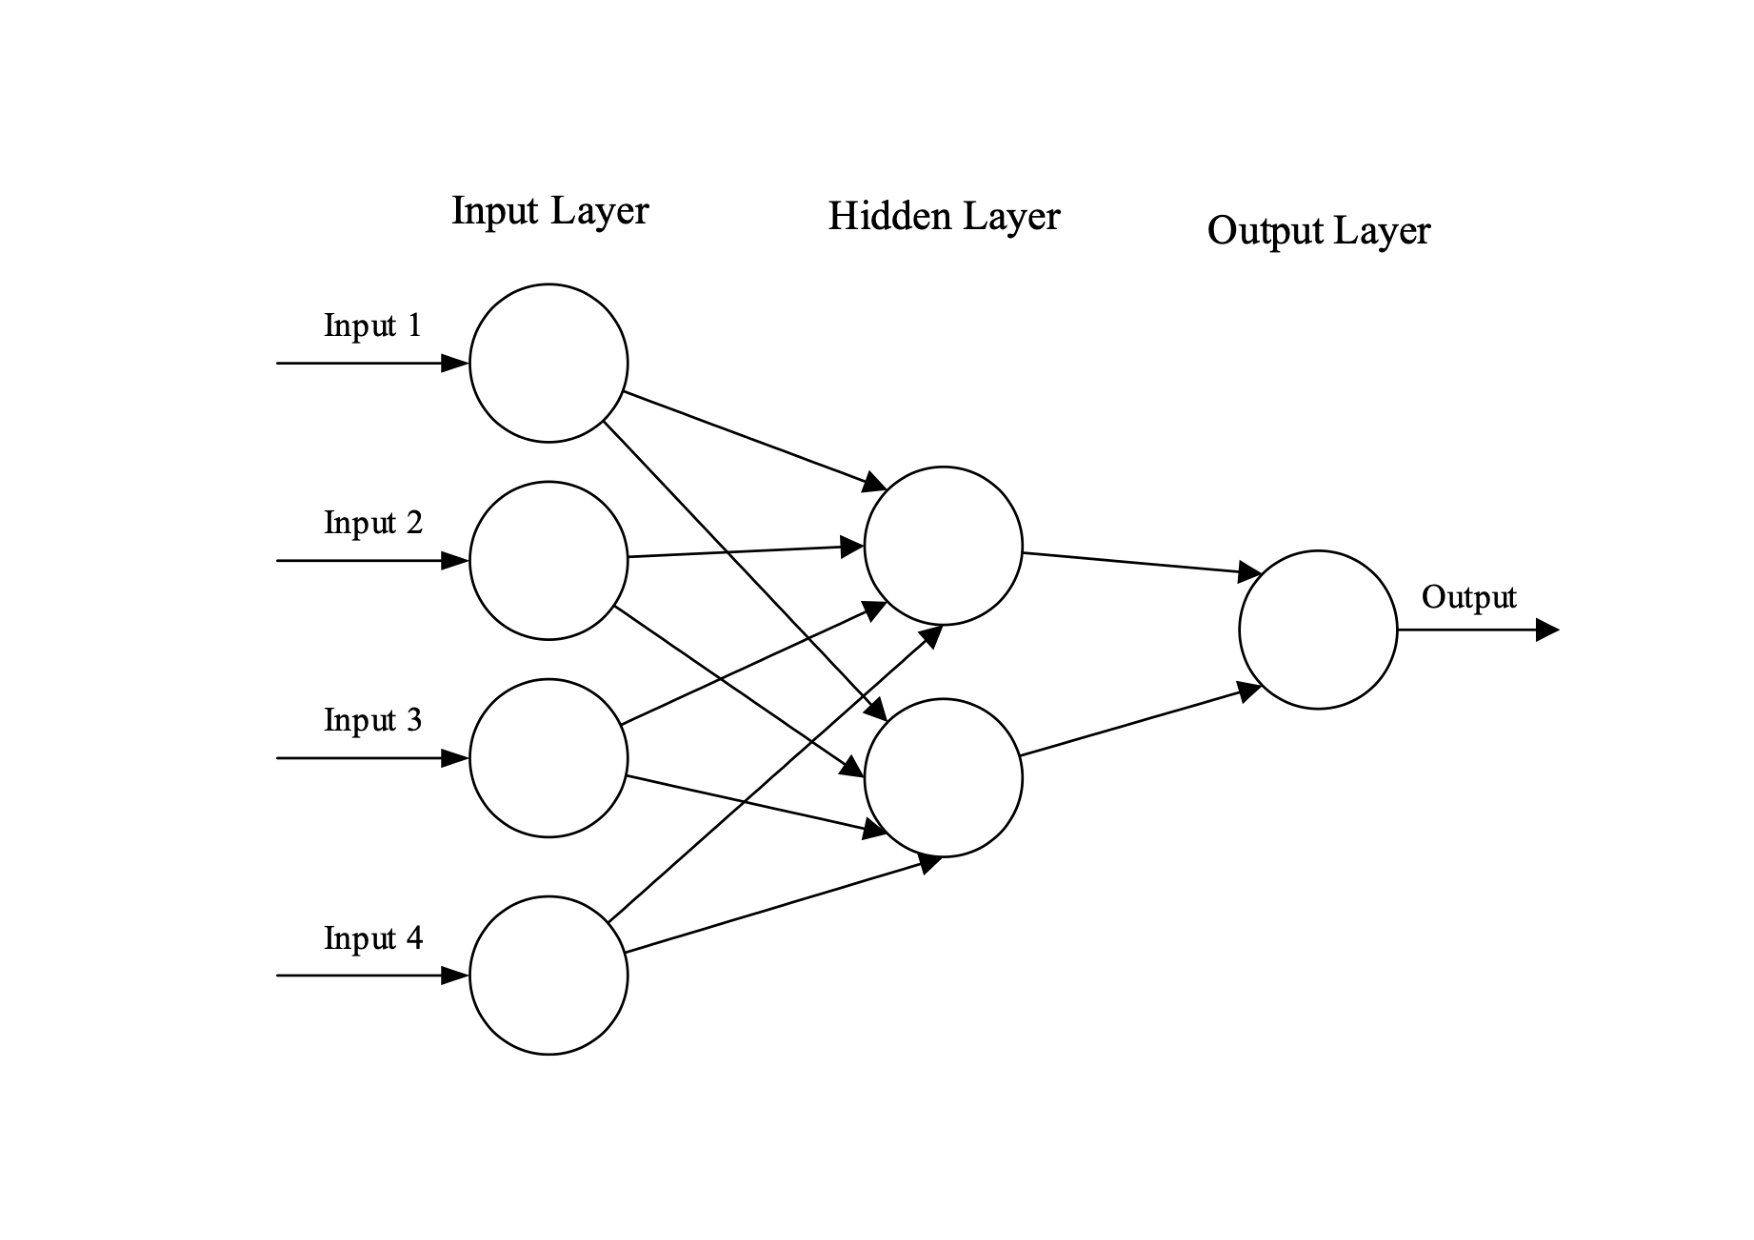
\includegraphics[width=0.8\linewidth]{img/ch2/simple-net}
   \caption[Feed-forward network example]{An example of a three-layer fully connected feed-forward network taken from~\cite{conv-intro}.}
    \label{fig:simple-net}
\end{figure}

Besides assigning a separate weight to each pair of neurons there are other possibilities of connecting neurons of consecutive layers.
Instead of assigning one weight to each pair of neurons, we can create a smaller weight matrix, often called filter or kernel which we reuse for multiple pairs of neurons. 
To do so, we perform convolution (i. e. a sliding dot product between the filter and a correspondingly sized part of the layer's input matrix). 
For visual explanation see Figure~\ref{fig:convolution}.
To arrive at a complete convolutional layer from the convolutional filter, more parameters need to be specified:
\begin{itemize}
    \item $W$  and $H$ - the width and height of the kernel
    \item $D$ the depth of the kernel. 
    It specifies how many input channels the layer's input has.
    What channels can represent can be illustrated for example on images.
    Imagine a colored image of size 32x32 pixels.
    Besides the width and height the image also has a 3rd dimesion specifying the RGB color. This third dimension are the channels, in this case three.
    Therefore, the dimension of the input (the image) is 32x32x3 and the kernel sliding over it has to have an additional dimension to handle the third input dimension. This additional dimension is the depth.
    \item $F$ - the number of output channels. 
    It specifies the number of different filters of size $WxHxD$ which all slide over the input giving $F$ output channels. 
    Similarly to the RGB channels of the input described above, each of the different filters allows the network to create its own representation of some feature of the layer's input.    
    \item \textit{stride} - it specifies by how many input points the kernel is shifted when sliding over the input. 
    \item \textit{padding} - specifies if only valid inputs should be taken into account or if the input is to be padded when the kernel reaches outside of the original input.
    If no padding is involved, the size of the output decreases along the dimension where kernel size of the filter is not 1.
\end{itemize}

Consider a 2D convolutional layer with input $I$ with $D$ input channels which is parametrized by a kernel $K$ of total size $WxHxDxF$. The output of this layer is computed as:

\begin{equation}
    (K * I)_{i,j,o} = f(\sum_{m,n,d} I_{i*s_1+m,j*s_2+n,c} K_{m,n,c,o})
    \label{eq:convolution}
\end{equation}

where $f$ is the activation function, $s_1$ and $s_2$ are strides in the corresponding dimensions, $c$ are the input channels and $o$ are the output channels.

\begin{figure}[!htpb]
\centering
   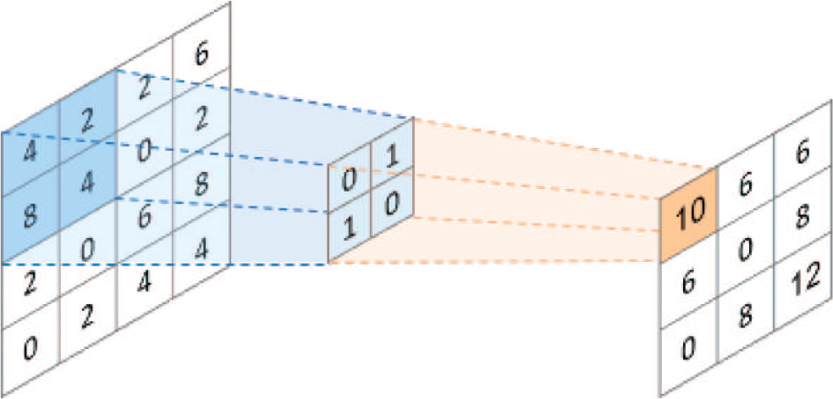
\includegraphics[width=0.8\linewidth]{img/ch2/convolution}
   \caption[Convolutional filter]{An example of a convolutional filter of width 2 and height 2 with weights 0, 1, 1, 0 sliding over an input of size 4x4 taken from~\cite{conv-diagram}}.
\label{fig:convolution}
\end{figure}

When a network contains one or multiple layers performing convolution, it is called a convolutional neural network (CNN).
Convolutional layers are often supplemented with pooling layers such as max-pooling or average pooling which aim to achieve shift-invariance in CNN architectures (\cite{cnn-description}). 
Common activation functions used in CNNs are sigmoid, tanh, or ReLU (\cite{relu-paper}).
A more recent and also popular activation is the ELU function which we are using in this thesis (\cite{clevert-elu-2016}). 

\subsubsection{Training}
Deep neural networks tend to have large numbers of parameters and therefore, cannot be trained analytically.
Instead, they are trained using fitting based methods.
These methods are variations of the gradient descent back-propagation algorithm (\cite{back-prop}).
Some popular variations are Stochastic gradient descent (\cite{sgd}), Adagrad (\cite{adagrad}) or more recently ADAM (\cite{kingma-adam-2017}).
To give the reader an idea of the fitting process, we describe it in a simplified manner. 
First a small subset of the input (a \textit{batch}) is randomly sampled from the training set. 
The batch is used as input into the network and is passed through the networks in a \textit{forward pass} to get the output of the network. 
The output and the \textit{gold labels} (desired output based on the selected inputs) are given to the \textit{loss function} which serves as a indicator of how far the model is from the correct output. 
Finally, the first derivatives of the loss function (the \textit{gradient}) with respect to the parameters (the \textit{weights}) of the model are subtracted from these parameters.
This allows moving in the direction of the steepest descent in the loss function value, in theory decreases the value of the loss function in the next forward pass.
To limit the size of the descent steps we use the \textit{learning rate} by which we multiply the gradient.
The forward pass is repeated for all batches in the dataset.
When all batches pass through the network, we can say one \textit{epoch} was completed.
The goal is to train a network for a number of epochs until it \textit{converges} to a low value of the loss function.

A low loss value on the training set means the model predicts the training data well.
Nevertheless, in order to see if the model is able to generalize over unseen data we keep another a portion of data - the validation set - out of training and only use it at the end of each epoch to estimate, how it performs on unseen data. 

\subsubsection{Regularization}
Overfitting - the adaptation to the training set distribution to an extend that the model does not generalize well over unseen data - is an unneglectable problem in deep neural networks including CNNs.
Multiple methods which effectively reduce this this problem have been proposed.
One option is to add a penalization term into the loss function which penalizes the model complexity.
An example of such a regularization is $l_p$-norm regularization (\cite{cnn-description}).
Dropout layers (\cite{drop-out}) also serve as regularization tools. 
By randomly dropping a portion of the connections between neurons, they prevent the network from becoming dependant on single neurons and force it to be able to make good predictions even when some information is absent.
Another popular regularization technique for CNNs is batch normalization (\cite{batch-norm}) which besides regularization also reduces the internal covariance shift. 
In CNNs this method now often substitutes dropout layers which are more suited for fully connected layers (\cite{cnn-description}).


\subsubsection{Dilated networks}\label{subsec:dilated-networks}
Convolutional neural networks are widely used in computer vision, more specifically in pattern recognition where they substantialy raised state-of-the-art (\cite{alexnet, dnn-computer-vision}) and their localized focus is well suited to image processing.
Nevertheless, CNNs are increasingly used for dense predictions.
Dense prediction in the sense of computer vision means assigning a label to each pixel of an image (\cite{dense-prediction-images}).
But this notion of one output per one input point can be extended to other fields such as machine translation (\cite{dense-prediction-machine-translation}), speech synthesis (\cite{angrick-speech-2018}) or prediction from EEG (\cite{schirrmeister-deep-2017}) and iEEG (\cite{Hammer-2021}).
The above mentioned tasks were solved using CNNs where an additional parameter called dilation was introduced (\cite{dense-prediction-images}).
Dilation inserts zeros between the elements of the convolutional filter and so enlarges the CNNs receptive field allowing it to cover more relevant information.
This way, the networks are more suitable for sequence processing (\cite{cnn-description}).
For a visual explanation of dilation see Figure~\ref{fig:dilation}.

\begin{figure}[!htpb]
\centering
   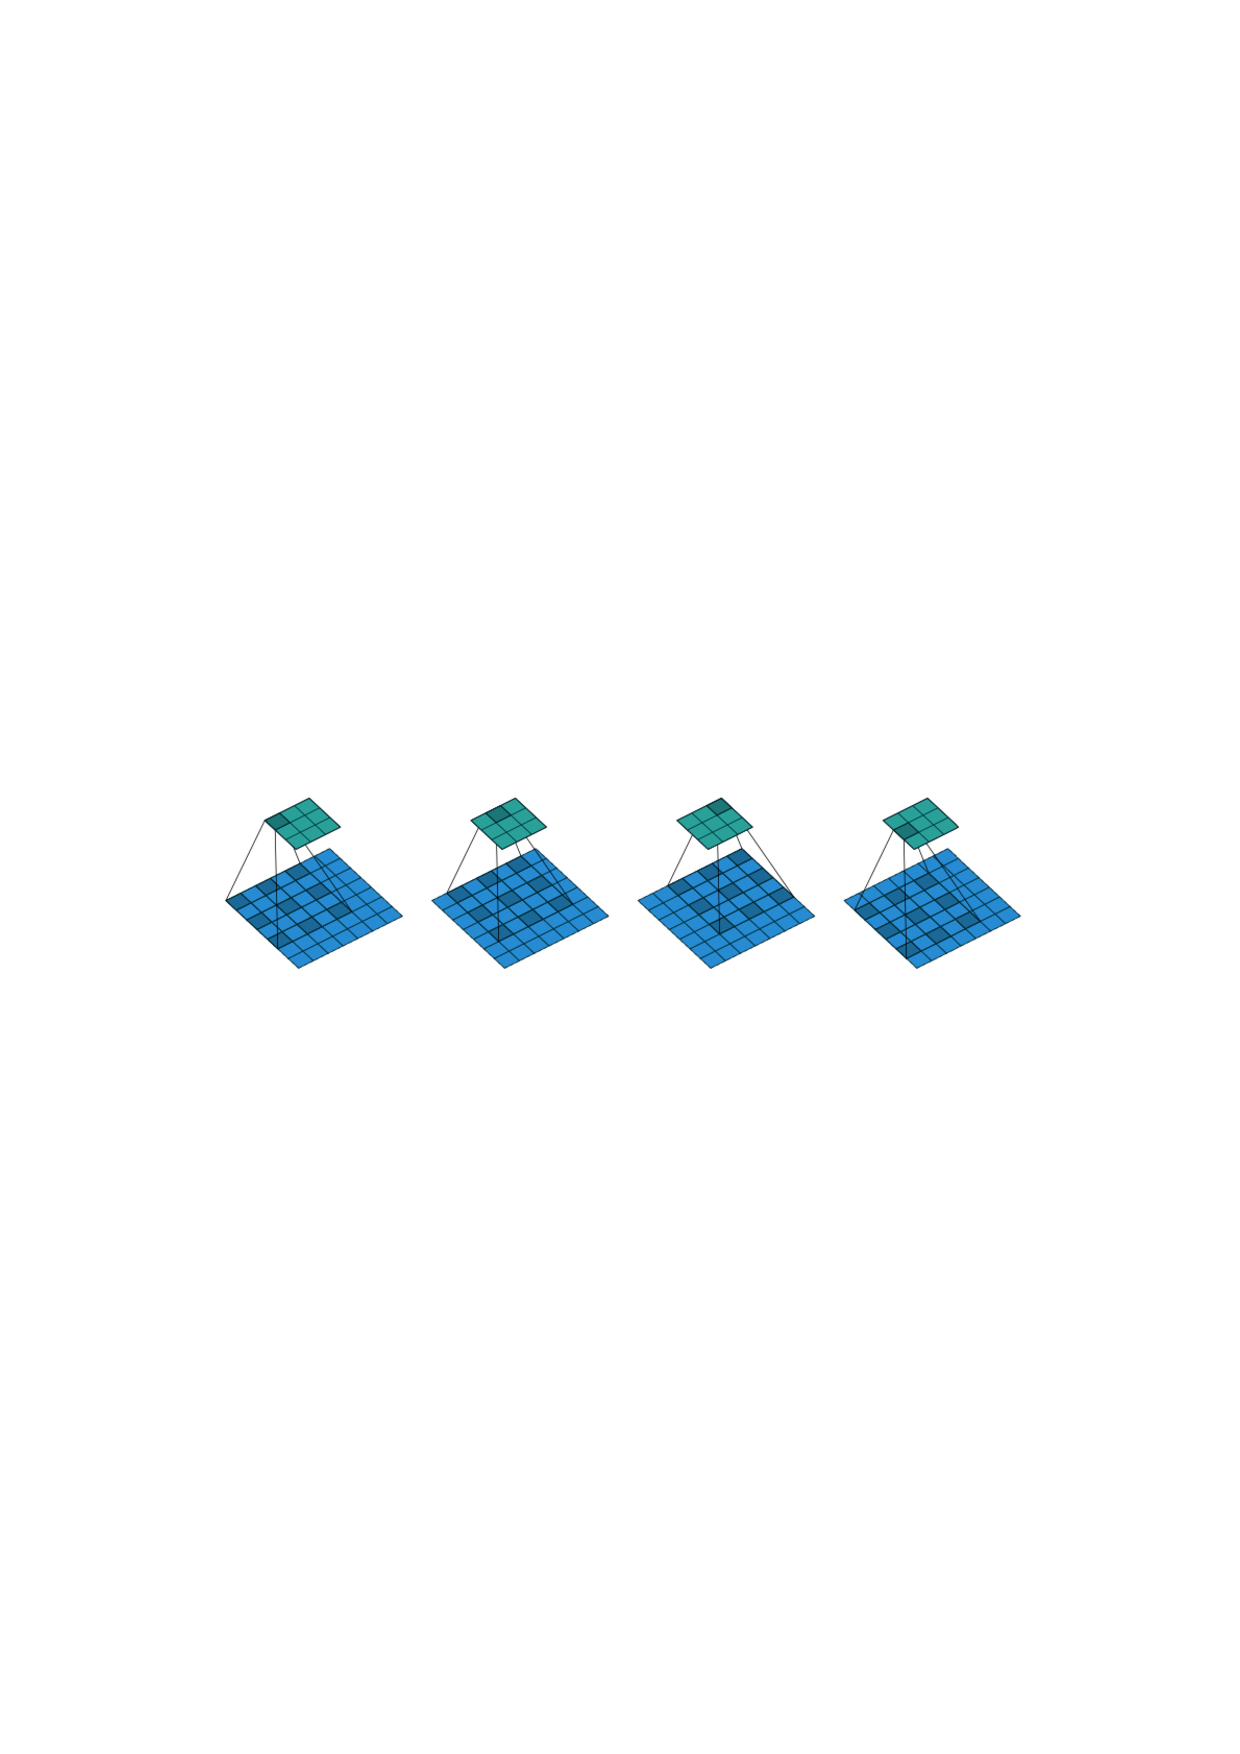
\includegraphics[width=0.8\linewidth]{img/ch3/dilated-conv}
   \caption[Dilated convolution]{An illustration of a dilated convolution with kernel size (3, 3) and dilation (2, 2) from \cite{dilated-conv}.}
   \label{fig:dilation}
\end{figure}


\subsection{CNN interpretability}\label{subsec:cnn-interpretability}
Poor interpretability of deep neural networks including CNN models has been identified as a major challenge limiting their usefulness across fields. 
Especially in safety-critical fields such as autonomous driving or medical decision support is it crucial for us to understand how DNNs arrive at their decisions.
And in the case of decoding from EEG and iEEG signals, understanding how networks which are able to translate these signals into for example velocity or speed arrive at their decision would lead to a better understanding of the brains functionality. 
It could also help identify ways in which these networks can be optimized to yield better predictions.
Because the strength of DNNs often lies in large datasets, in a field where data is less available, such optimizations are particularly important.

Substantial effort has been made to explain how deep neural networks make their predictions.
Many of the popular methods, such as maximal activating inputs (\cite{maximizing-activation}), class-activation maps (\cite{class-activation-maps}), saliency maps (\cite{gradient-visualization}) or layer-wise relevance propagation (\cite{sturm-interpretable-2016}) have been used also in interpreting DNNs used for brain signal decoding (\cite{goodfellow-towards-2018, hartmann-hierarchical-2018, rieke-visualizing-2018, yang-visual-2018,  sturm-interpretable-2016,}).

\section{DNNs for (i)EEG decoding}
\label{sec:dnn-decoding}
In this section, we introduce the Deep4Net proposed by~\cite{schirrmeister-deep-2017} which is the main focus of the presented experiments.
Then we go on to describe another paper - by~\cite{Hammer-2021} - who used the Deep4Net to solve the same task as we are solving in this thesis on the same data and laid the foundation of the here presented research.

\subsection{Schirrmeister et al.}\label{subsec:schirrmeister-et-al}
The paper by~\cite{schirrmeister-deep-2017} introduced multiple CNN and hybrid architectures suitable for movement decoding from raw EEG signals, including the Deep4Net.
It has several important contributions.
First of all, it shows that CNNs are able to achieve at least as good performance on classification from raw EEG signals as the widely used Filter bank common spatial patterns (FBCSP) do from manually extracted features.
Besides that, it shows that recent advances in machine learning such as batch normalization or the exponential linear unit (ELU) transfer function help boost the decoding accuracies of networks used for movement decoding task.
Lastly, using a perturbation visualization method they explore, which spectral power features are important for the network's predictions.
They show a substantial effect of the frequencies in the alpha and beta band and also also observe an effect of the high-gamma freuquencies on the predictions which, they claim, is for the first time when using non-invasive EEG data.

\subsubsection{Classification task}
Multiple datasets were used to estimate the abilities of the introduced architectures.
One was the BCI IV 2a competition dataset (\cite{brunner2008bci}) where the task was to classify whether the participants (9 in total) imagine to move the right hand, left hand, both feet or tongue.
The second dataset they used was one they acquired in their lab called High Gamma dataset (HGD) because it is especially well-suited for extracting information from high frequencies.
Two additional datasets were used to determine if the main results hold also on other datasets. 
To this extend the BCI IV 2b competition and the Mixed Imagedy Dataset (MID) were used and confirmed their findings. More details about the datasets can be found in the supplementary material for this paper.


\subsection{Hammer et al.}\label{subsec:hammer-et-al}
In 2021~\cite{Hammer-2021} used the Deep4Net architecture for regression on intracranial EEG.
Differing from the original Deep4Net paper not only in the type of task but also in the data type, they inspected the performance and features of the architecture in these altered settings.
They visualized the important spectral features investigating learnt specialization of single network units to either phase or amplitude.
This thesis directly follows up on their research.

\subsubsection{Regression task and performance}
In this paper, Deep4Net was used to predict kinematic variables, namely velocity and absolute velocity (speed) based on intracranial EEG (iEEG) of subjects undergoing pre-surgical epilepsy screening.
The subjects were asked to play a simple video game.
Their task was to use a joystick to control a car moving forward on a winding track.
The joystick allowed for left and right movement and the velocity and absolute velocity of this movement were recorded along with concomitant iEEG signals. 
The dataset and the task are described in more detail in Section~\ref{subsec:ieeg-data-preprocessing}.

Unsurprisingly, the Deep4Net significantly outperformed linear regression used as a baseline on this task, especially for absolute velocity as is apparent from Figure~\ref{fig:hammer-performance}.
The dataset is not public, therefore, a comparison to more decoding methods is not possible, nevertheless, the correlation values it achieved are quite high.

\begin{figure}[!htpb]
\centering
   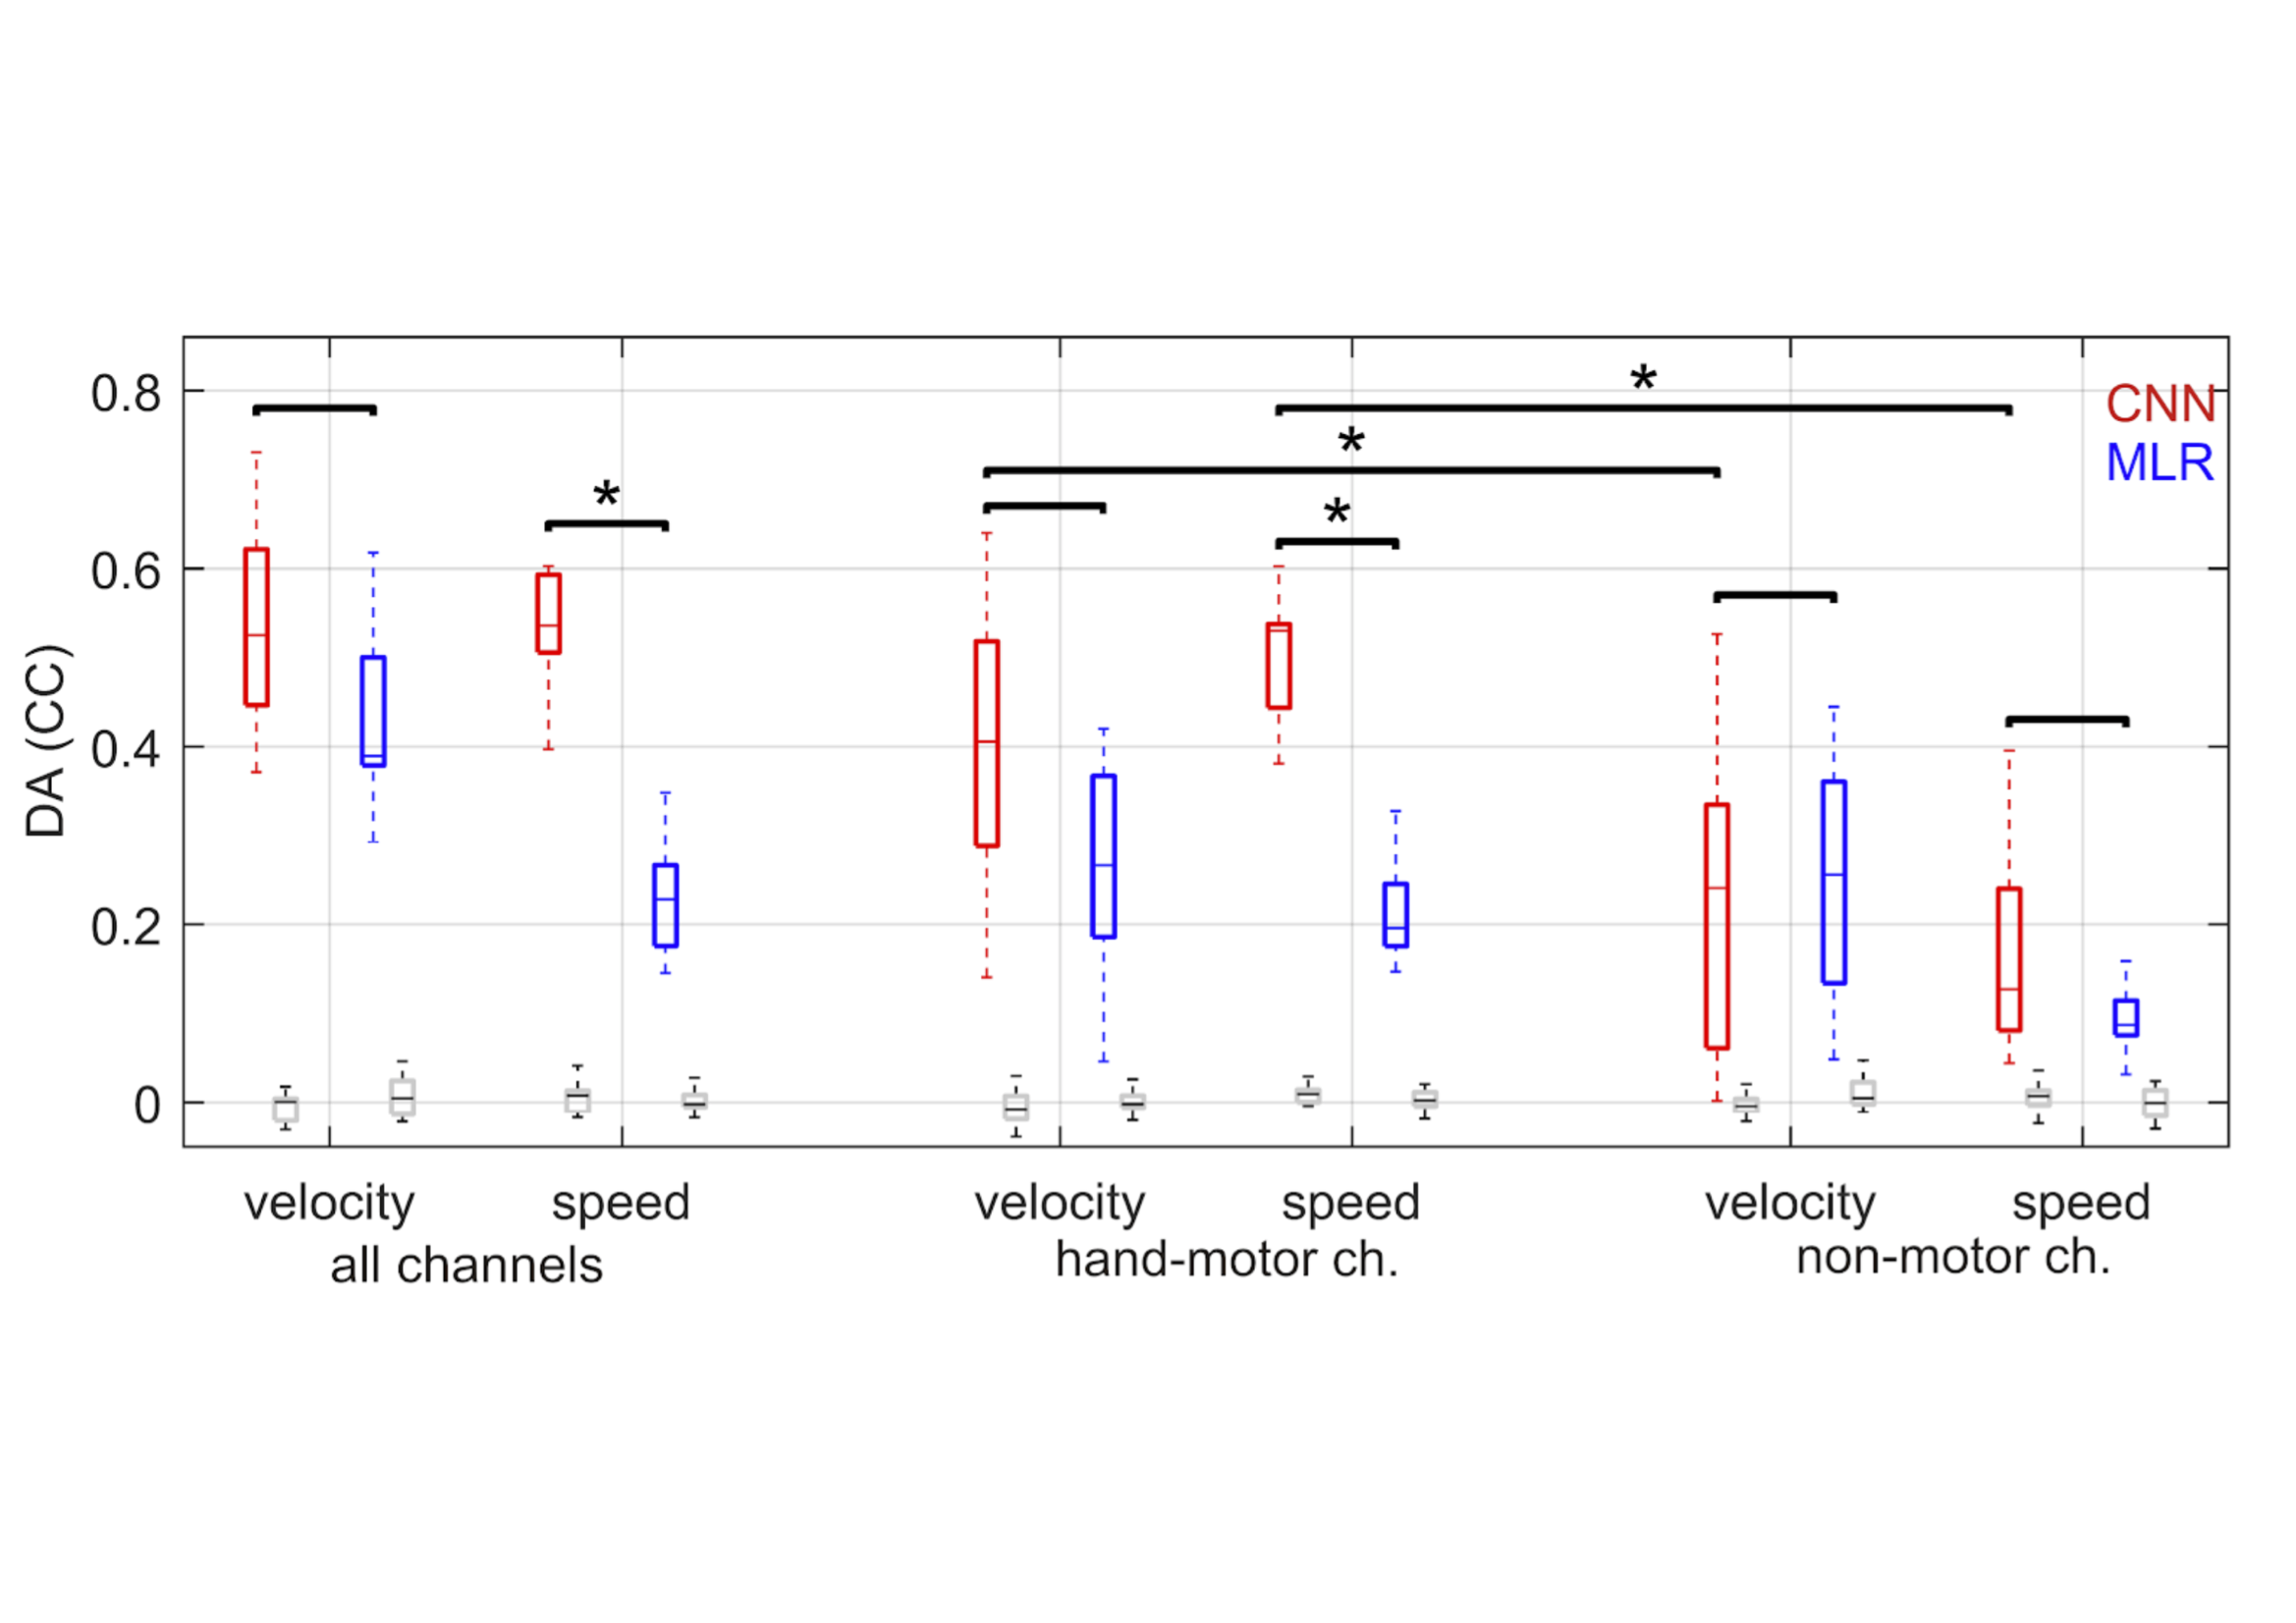
\includegraphics[width=0.8\linewidth]{img/ch2/hammer-decoding-acc}
   \caption[Orignial Deep4Net performance]{"The decoding models for both the Deep4Net (CNN) and multi-linear regression (MLR) used iEEG data from all channels, hand-motor channels, or non-motor channels (see Section~\ref{subsec:separation-of-motor-and-non-motor-channels}.
   The performance was assessed by correlation coefficients (CCs) between predicted and real kinematic parameters.
   In each box-plot, the box indicates the interquartile range (IQR) of the DA distribution across participants, the median is marked by a horizontal line inside the box, the whiskers indicate 1.5-times the IQR.
   The chance-level CCs for shuffled datasets was assessed for both CNN and MLR (grey box-plots below)"~\cite{Hammer-2021}}
    \label{fig:hammer-performance}
\end{figure}

\subsubsection{Training regime}
The Deep4Net was trained using the ADAM optimizer with learning rate 0.01 for 100 epochs.
To calculate the error of the network's predictions, the mean squared error (MSE) was used as the loss function.
A leave-one-out-cross-validation on 25 second long data segments (see Section~\ref{subsec:ieeg-data-preprocessing} was employed to estimate performance.
The goodness of prediction was evaluated on the one fold not included in training using the linear Pearson's correlation coefficient (\cite{pearson-vii-1895}).
Chance level performance was assessed by randomly pairing the inputs and gold labels.
For example iEEG data from fold 2 were paired with gold kinematic data from fold 6.

\subsubsection{Input perturbation - output correlation visualization}
The perturbation analysis in~\cite{Hammer-2021} was more thorough than in the case of~\cite{schirrmeister-deep-2017}
Besides looking at the influence of amplitude perturbations, they also investigated the influence of phase perturbations, similarly to~\cite{hartmann-hierarchical-2018}.
Moreover, attention was paid to the specialisation of single units to either phase or amplitude.
While most findings were in line with previous literature, the low sensitivity of the network to high-gamma frequency bands amplitudes was unexpected.
Especially considering two things: 
1. This same architecture was able to use high-gamma information in EEG decoding where high frequencies contain more noise than in iEEG signal in~\cite{schirrmeister-deep-2017}.
2. High-gamma has been shown to be informative in for absolute velocity decoding on a subset of the same data when using linear regression in~\cite{hammer-predominance-2016}.


\subsection{Related work}
In this section we describe more works which are relevant for movement decoding from EEG or iEEG using deep learning, but are not directly used or referenced in our experiments.
We specifically introduce a few other neural network architectures which have been employed to decode movement related variables.

One such networks is the EEGNet from~\cite{lawhern-eegnet-2018}.
The authors build a CNN architecture which is able to generalize over different BCI paradigms.
They show that the EEGNet is able to learn a wide variety of interpretable features over a range of different EEG decoding tasks including movement related cortical potentials and sensory motor rhythms.

An architecture idea recently repeatedly used for decoding from EEG and iEEG signals is combining recurrent layers and convolutional layers to form a hybrid networks.
Examples of utilizing such networks in movement-related paradigms are for example~\cite{xie-cnn-lstm-finger-movement, Zhang-2019}.
In~\cite{xie-cnn-lstm-finger-movement} a network constituting of 4 convolutional layers followed by one long-short term memory (LSTM)~(\cite{lstm-paper}) layer was utilized to decode individual finger flexion.
In~\cite{Zhang-2019}, three convolutional layers followed by three LSTM layers were utilized to solve the BCI IV 2a competition task (same as in~\cite{schirrmeister-deep-2017}).



\chapter{Methodology}\label{ch:methodology}
In this chapter, we go over the details and specifics of the dataset and the methods used in this thesis.
We first provide information related to the dataset and then give a detailed description of the Deep4Net architecture together with information about the training regime.
We also describe the gradient visualization method which we chose to interpret the decisions of the CNNs.

\section{Dataset}\label{sec:dataset}
The dataset was the same as in the unpublished study of~\cite{Hammer-2021}.
Modified with the authors permission, the description of the experiment settings, and the pre-processing follows.

\subsection{Movement task and kinematic variables}\label{subsec:movement-task-and-kinematic-variables}
A dataset that was already used in several other iEEG studies to examine decoding of movement kinematic parameters (\cite{Hammer-2021,hammer-predominance-2016,hammer-role-2013}) was utilized for the purposes of this thesis.
The participants performed a motor task based on driving a car in a computer simulation.
They controlled the position of the car on a computer screen using a steering wheel which they held in both hands.
The task was to keep the car on a curved road.
The road was random without any repetitions, following a low-pass filtered white noise trajectory.
During the movement task, the position of the car on the road was measured.
The position of the car linearly corresponded to the deflection of the steering wheel and was measured relative to the screen center, which corresponded to zero-deflection of the steering wheel.
Importantly, the control of the car's position was possible only in the horizontal dimension (left - right).
The upward movements of the car (vertical scrolling speed) were kept constant in each run of the game and adjusted for each subject individually.

The difficulty and the recording time of each subject was also adjusted based on the participant's motivation/ability to participate, lasting 25 $\pm$ 7 min (mean $\pm$ SD).
The car game difficulty was modified by the vertical scrolling speed of the car.
Therefore, to account for faster movements, the low-pass cutoff frequency was set to 10~Hz for smoothing the raw tracker data prior to the derivation of the kinematic parameters.

From the horizontal - 1-D trajectory, the following two kinematic parameters were derived:
1. velocity computed as a derivative of position, 2. speed as the absolute value of velocity.
Velocity thus contained the directional information in its sign;
specifically, velocity values smaller than zero implicated movement to the left and vice versa, while speed indicated how fast the car was moving left or right (irrespective of its direction).
The time-series of the kinematic parameters were resampled at 250~Hz and temporally aligned to the iEEG data.

\subsection{Recording}\label{subsec:recording}
The recordings were performed in the University Medical Centre in Freiburg, Germany and in the Motol University Hospital in Prague, Czech Republic.
The study included 12 epilepsy patients (6 male, age 19--50,  33 $\pm$ 10, (mean $\pm$ SD ) all of which had intracranial EEG implantations.
Some of the implantations were placed in the region of the motor cortex.
The location of the electrodes was dependent solely on the needs for medical evaluation of their medication-resistant epilepsy.
Both sEEG and ECoG electrodes were present among patients.
Detailed information about electrode type and placement is presented in Table\ref{tab:patient-table} and Figure\ref{fig:electrodes}.

\begin{figure}[!htbp]
\centering
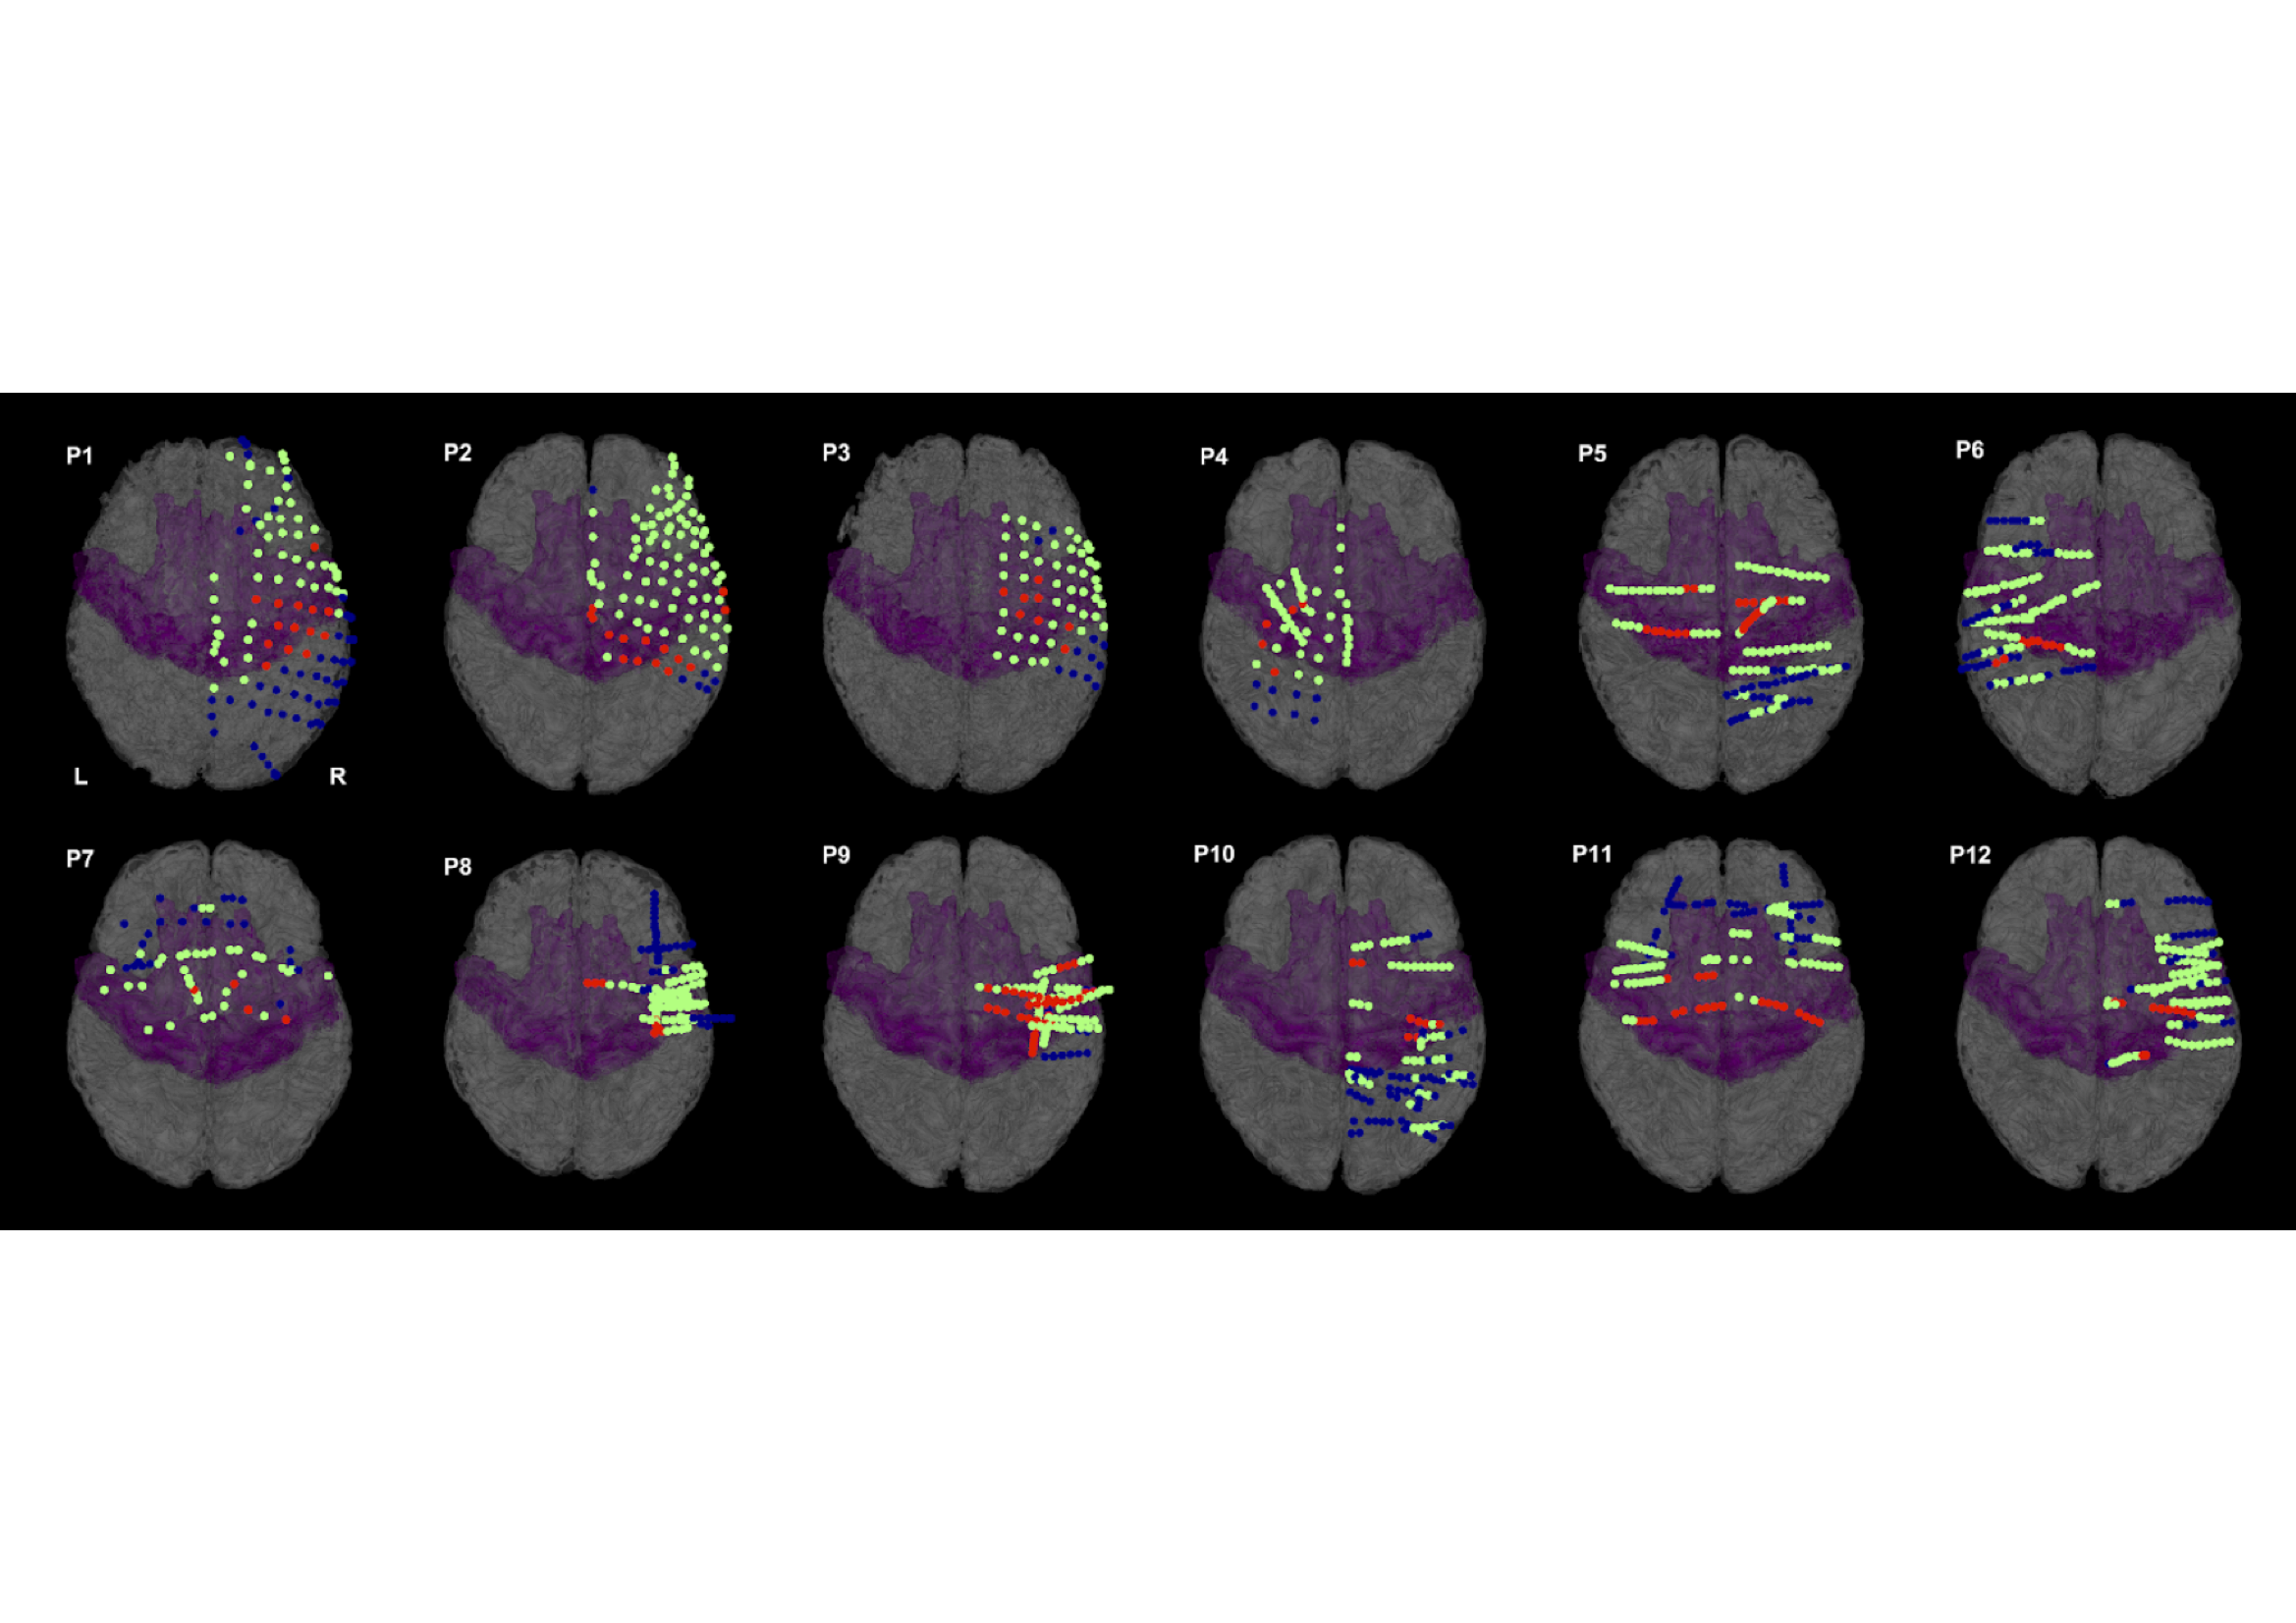
\includegraphics[width=0.8\linewidth]{img/ch3/electrodes}
\caption[Implantation schemes]{Implantation schemes of the 12 patients (P1 - P12) taken from~\cite{Hammer-2021}. The motor cortex is highlighted in magenta (defined as the union of areas 4 and 6 of the SPM Anatomy Toolbox). The electrodes are color-coded in the following way: Red - channels with hand-motor response after electrical stimulation mapping; dark blue - non-motor channels; green - other channels.}
\label{fig:electrodes}
\end{figure}

\begin{table}[!htbp]
\centering
\begin{tabular}{|p{1.25cm}|p{0.95cm}|p{1.75cm}|p{1.65cm}|p{1.65cm}|p{0.5cm}|p{0.65cm}|p{0.6cm}|p{0.8cm}|}
\toprule
Patient&Sex (Age)&Pathology&Implant loc&Electrode type ($N$) & $N_r$ & $N_{ch}$ & $N_{m}$ & $N_{nm}$ \\
\hline
\midrule
P1 & F (47) & CG & Right frontal & ECoG (98),  sEEG (12) & 25 & 85 & 14 & 47 \\
\hline
P2 & M (48) & FCD & Right fronto-temporal & ECoG (90), sEEG (12) & 53 & 49 & 15 & 11 \\
\hline
P3 & M (50) & CG & Right frontal & ECoG (64) & 3 & 61 & 8 & 11 \\
\hline
P4 & F (22) & FCD & Left frontal & ECoG (40),  sEEG (12) & 11 & 47 & 5 & 16 \\
\hline
P5 & F (29) & Gilosis & Left and right fronto-parietal &  sEEG (125) & 10 & 115 & 23 & 29 \\
\hline
P6 & M (29) & FCD & Left frontal &  sEEG (125) & 34 & 91 & 9 & 39 \\
\hline
P7 & F (32) & FCD & Left and right insular &  sEEG (61) & 14 & 47 & 4 & 22 \\
\hline
P8 & M (19) & FCD & Right insular &  sEEG (117) & 16 & 101 & 9 & 36 \\
\hline
P9 & F (25) & Gliosis & Right insular &  sEEG (117) & 21 & 96 & 35 & 12 \\
\hline
P10 & M (34) & FCD & Right fronto-parietal &  sEEG (125) & 23 & 102 & 8 & 63 \\
\hline
P11 & M (34) & FCD & Left and right frontal &  sEEG (126) & 11 & 115 & 21 & 48 \\
\hline
P12 & M (28) & Not operated & Right frontal &  sEEG (125) & 20 & 105 & 10 & 27 \\
\bottomrule
\end{tabular}
\caption[Patient details]{$N_r$, $N_{ch}$, $N_{m}$, $N_{nm}$  : number of rejected, non-reject, hand-motor, and non-motor channels, respectively. FCD: focal cortical dysplasia; CG: Cryptogenic.}
\label{tab:patient-table}
\end{table}

\subsection{Separation of motor and non-motor channels}\label{subsec:separation-of-motor-and-non-motor-channels}
The separation of the channels was not a part of this thesis. 
We already obtained separated channels.
The specific separation criteria are described below as provided by~\cite{Hammer-2021}. \\

One of the aims of the~\cite{Hammer-2021} study was to show what the CNNs learned from the raw brain signals.
The hypothesis was that the CNNs would focus on information from the hand-motor cortex when solving a movement-related task.
To verify this hypothesis, the recorded channels were divided into two distinct, non-overlapping groups: 1. hand-motor channels and 2. non-motor channels.
The hand-motor channels induced a clear hand motor response after the electrical stimulation at low intensities underneath or around the electrode contacts.
The non-motor channels, on the other hand, produced no sensory/motor response after the stimulation.
Furthermore, a requirement of at least 1 cm distance from the motor and pre-motor areas (i.e. Area 4a, Area 4p and Area 6 from the SPM Anatomy toolbox\cite{eickhoff-new-2005}) had to be satisfied for a channel to be included in the non-motor group.
To this end, all MRI brain scans (T1-weighted sequence) were normalized to the MNI space and the electrodes' coordinates were read out from either the post-implantation MRI or CT scans53. \\

The average number of hand-motor channels was 13 $\pm$ 9 (mean $\pm$ SD), while there were 29 $\pm$ 18 (mean $\pm$ SD) non-motor channels.
Some electrodes did not fall into either of the hand-motor and non-motor channel groups (e.g. channels in the motor cortex the electrical stimulation of which induced leg-motor response).
These electrodes were then left out in some analysis, because the aim was to delineate the difference between the two distinct groups of channels (the hand-motor channel group and the non-motor channel group clearly far away from the motor cortex).



\subsection{IEEG data preprocessing}\label{subsec:ieeg-data-preprocessing}
The iEEG data pre-processing was also already completed when we obtained the dataset and it was not carried out as a part of this thesis.
Nevertheless, we provide the description of pre-processing from ~\cite{Hammer-2021}.
A comprehensive rejection of \textit{epileptic} channels based on the information from the respective epilepsy centers was performed, because the primary aim was to investigate the physiological brain activity.
Thus, the channels, i.e. those located in the seizure onset zone and/or containing a large number of inter-ictal epileptiform discharges, were rejected from this study (20 $\pm$ 13, mean $\pm$ SD) over subjects; see Table \ref{tab:patient-table}.
All non-rejected iEEG channels (85 $\pm$ 28, mean $\pm$ SD) were referenced to their common average (CAR), high-pass filtered at 0.15~Hz (3rd order Butterworth filter), normalized to the inter-quartile range of each channel, and resampled to 250~Hz, to yield consistent data sets from the different recording systems used at both aforementioned epilepsy centers\footnote{Motol University Hospital and University Medical Centre Freiburg}.
The iEEG data were resampled to 250~Hz in order to emulate the same setup of the Deep4Net from~\cite{schirrmeister-deep-2017}, which was successfully applied to demonstrate high-gamma (70 - 90~Hz) effects in decoding motor behaviour from non-invasive EEG. Importantly, any over-fitting in the pre-processing was carefully avoided (i.e., all parameters of the pre-processing of the test set were estimated on the training set) and only causal, finite impulse response filters were applied.
Therefore, the decoding approach could be readily applied also in a closed-loop, online BMI.

The aligned iEEG and kinematic time-series were divided into 25-s long data segments.
In order to minimize a potential influence of temporal correlations in neighbouring data parts, the segments had a 2-s margins in between each other.
Additionally, the last two minutes of the recordings were left as a test set.
The test set was not a part of the dataset that was utilized in this thesis.


\subsection{Multiple dataset conditions}\label{subsec:modifications-to-the-dataset}
In this thesis, we refer to multiple variations of the original dataset provided by the Motol University Hospital.
Following modifications were explored:
1. filtering out certain frequencies, 2. shifting the predicted time-point with respect to the input window, 3. spectral whitening.
\begin{itemize}
\item \textbf{Filtering} We created two types of datasets using filtering.
A \textit{high-pass filtered dataset} using a 15th order Butterworth filter, cut-off frequency 60~Hz, non-zero phase shift and a \textit{low-pass filtered dataset} using a Butterworth filter order 15, cut-off frequency 40~Hz, non-zero phase shift.
Besides full training on these datasets, parts of these datasets were combined for training and validation to see how a network trained on full data performs on high-passed data etc.
\\

\item \textbf{Shifting} Originally in~\cite{Hammer-2021} the dataset was constructed so that the predictions were made from signals recorded prior to their execution (causal prediction).
In addition to this, we also created datasets where the labels (i.e. values of kinematic variables) were shifted so that predictions were made also from signals recorded after movement execution (acausal prediction).
While a network trained in this manner is unsuitable for online BCI, it allows us to inspect which time frame of the signails contains information about the movement.
More details about how the shift influences the predictions and why can be found in~\ref{subsec:receptive-field}. \\

\item \textbf{Spectral whitening} Lastly we also created whitened datasets.
Spectral whitening normalizes amplitudes of all frequencies to one.
It was achieved using a Fourier transformation of each 25s long segment (which the dataset was divided to) into the power spectrum, obtaining information about phase and amplitude.
Then dividing the amplitudes with their absolute value and then, via inverse Fourier transformation, transforming it back to signal.
The whitened signal was normalized to its inter-quratile range (IQR).
This normalization was calculated and applied to each segment on the training set and the same parameters averaged over all 25s long segments of the training set were applied to the validation set.
Figure~\ref{fig:spectral-whitening} illustrates the effects on a portion of one of the 25s long segments.
\end{itemize}

\begin{figure}[!htbp]
\centering
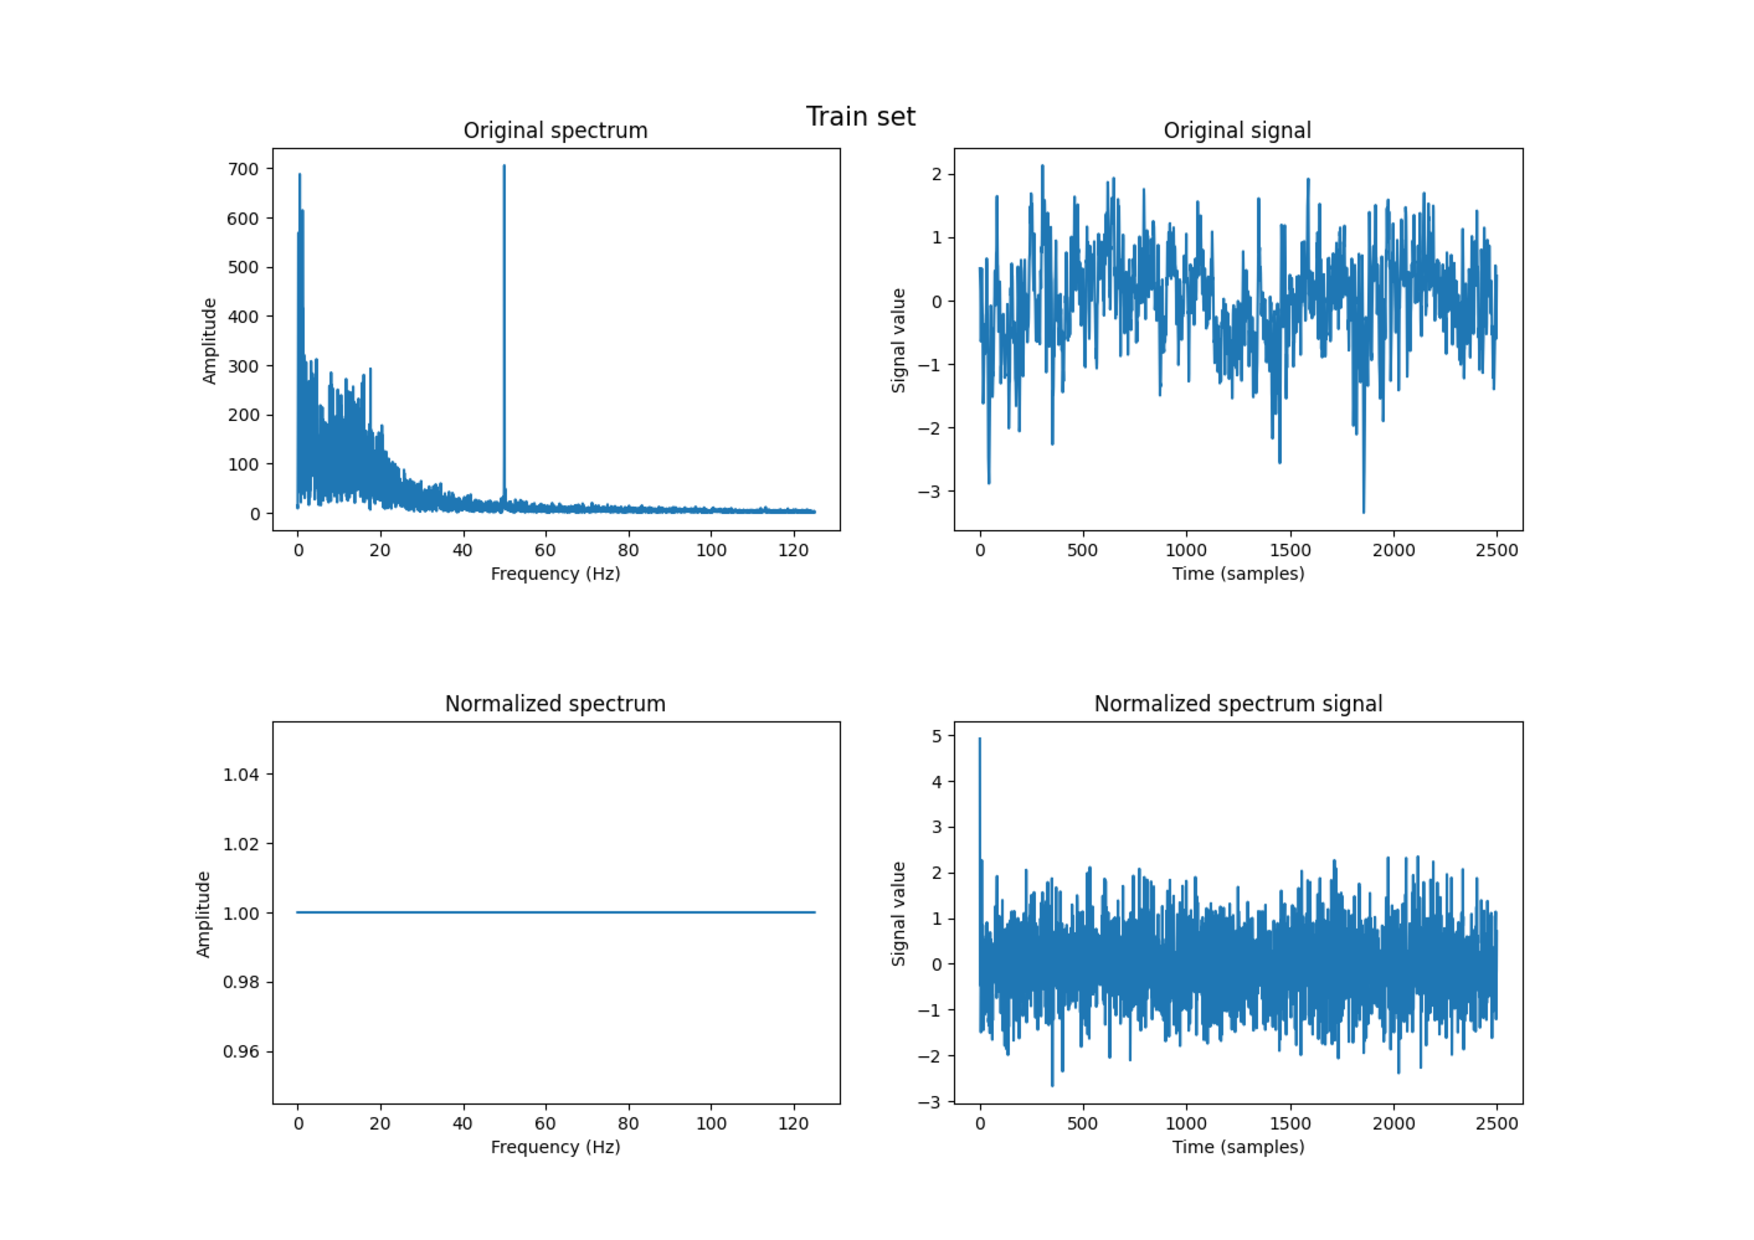
\includegraphics[width=\linewidth]{img/ch3/spectral-whitening}
\caption[Spectral whitening]{The top row shows the original power spectrum of the iEEG signal and the original iEEG signals of the 10 seconds of the first 25s long segment.
The bottom row shows how spectral whitening changed both the spectrum and the signal.}
\label{fig:spectral-whitening}
\end{figure}


\section{Deep4Net}\label{sec:deep4net}
The Deep4Net, which is freely available in the Braindecode library\footnote{www.braindecode.org}, was already shortly described in Section~\ref{subsec:schirrmeister-et-al}.
In this section, we describe it in more detail. 
Besides the describing the architecture as used in~\cite{Hammer-2021} we focus on how cropped decoding is used (Section~\ref{subsec:cropped-decoding}), what the receptive field of the network looks like and how it affects the predictions (Section~\ref{subsec:receptive-field}), we describe the training procedure (Section~\ref{subsec:training}), the visualization of the networks' gradients~\ref{subsec:gradinet-visualization} and architectural modifications we introduce in this thesis Section~(\ref{subsec:architectural-modifications}). Lastly we also state how performance is analyzed Section~(\ref{subsec:performance-analysis}).


\subsection{Architecture}\label{subsec:architecture}
The architecture has been previously used in a number of EEG decoding tasks~(\cite{Hammer-2021, schirrmeister-deep-2017, hartmann-hierarchical-2018}).
It is implemented in the PyTorch framework\footnote{https://pytorch.org}.
The input of the network is a 2D array with time-steps along one axis and channels along the other axis.
The architecture consists of four convolutional-max-pooling blocks and one final convolutional layer.
It is designed so that a special first block can learn spatially global filters.
The following three standard blocks (conv\_2 - conv\_4) then allow for learning temporal hierarchies of local and global modulations (\cite{schirrmeister-deep-2017}).
The first convolutional block is split into two parts.
One performs convolution over time (conv\_temp) and the second over the channels with weights for all possible electrode pairs using filters of the preceding temporal convolution (conv\_spat).
Because there is no activation function between these two layers, they could be merged, but the authors emphasize the regularization function of this separation because it forces a separation of the linear transformation into a temporal convolution and a spatial filter.

A convolutional block of the Deep4Net starts with a convolutional layer, then a batch normalization layer follows, after which a non-linearity is added, in the case of the Deep4Net it is the exponential linear unit (ELU) function.
Finally, a max-pool layer closes the convolutional block.
An output layer, which originally was a softmax, comes last.
To use this network for a regression task that the present thesis focuses on, only a single modification needs to be done: removing the last softmax layer and replacing it with a convolutional layer.
This last layer is called the conv\_classifier.
The architecture already transformed for regression is depicted in Figure~\ref{fig:architecture}.

The Deep4Net is able to process varying input lengths.
In each convolutional layer it simply slides its filters over the input and gives a respective number of outputs.
Therefore, before training, the number of outputs needs to be calculated based on the size of the input window that was chosen.
The corresponding values (gold labels) of the predicted kinematic variables are cropped accordingly.
In this thesis, we used 1200 samples as input window length which corresponds to 4.8 seconds.
For the Deep4Net as used in~\cite{Hammer-2021} a window of 1200 samples gives 679 predictions.
Therefore, one prediction is made from $11200 - 679 + 1 = 522 $ samples.
These samples are recorded before execution of the predicted movement which makes the network suitable for online BCI.


Lastly we point out, that the network does not use any padding. 
This makes its receptive field non-uniform and we discuss the consequences in Section~\ref{subsec:receptive-field}.
Nevertheless it is necessary to avoid padding to perform cropped decoding described in Section~\ref{subsec:cropped-decoding}.

\begin{figure}[!htbp]
\centering
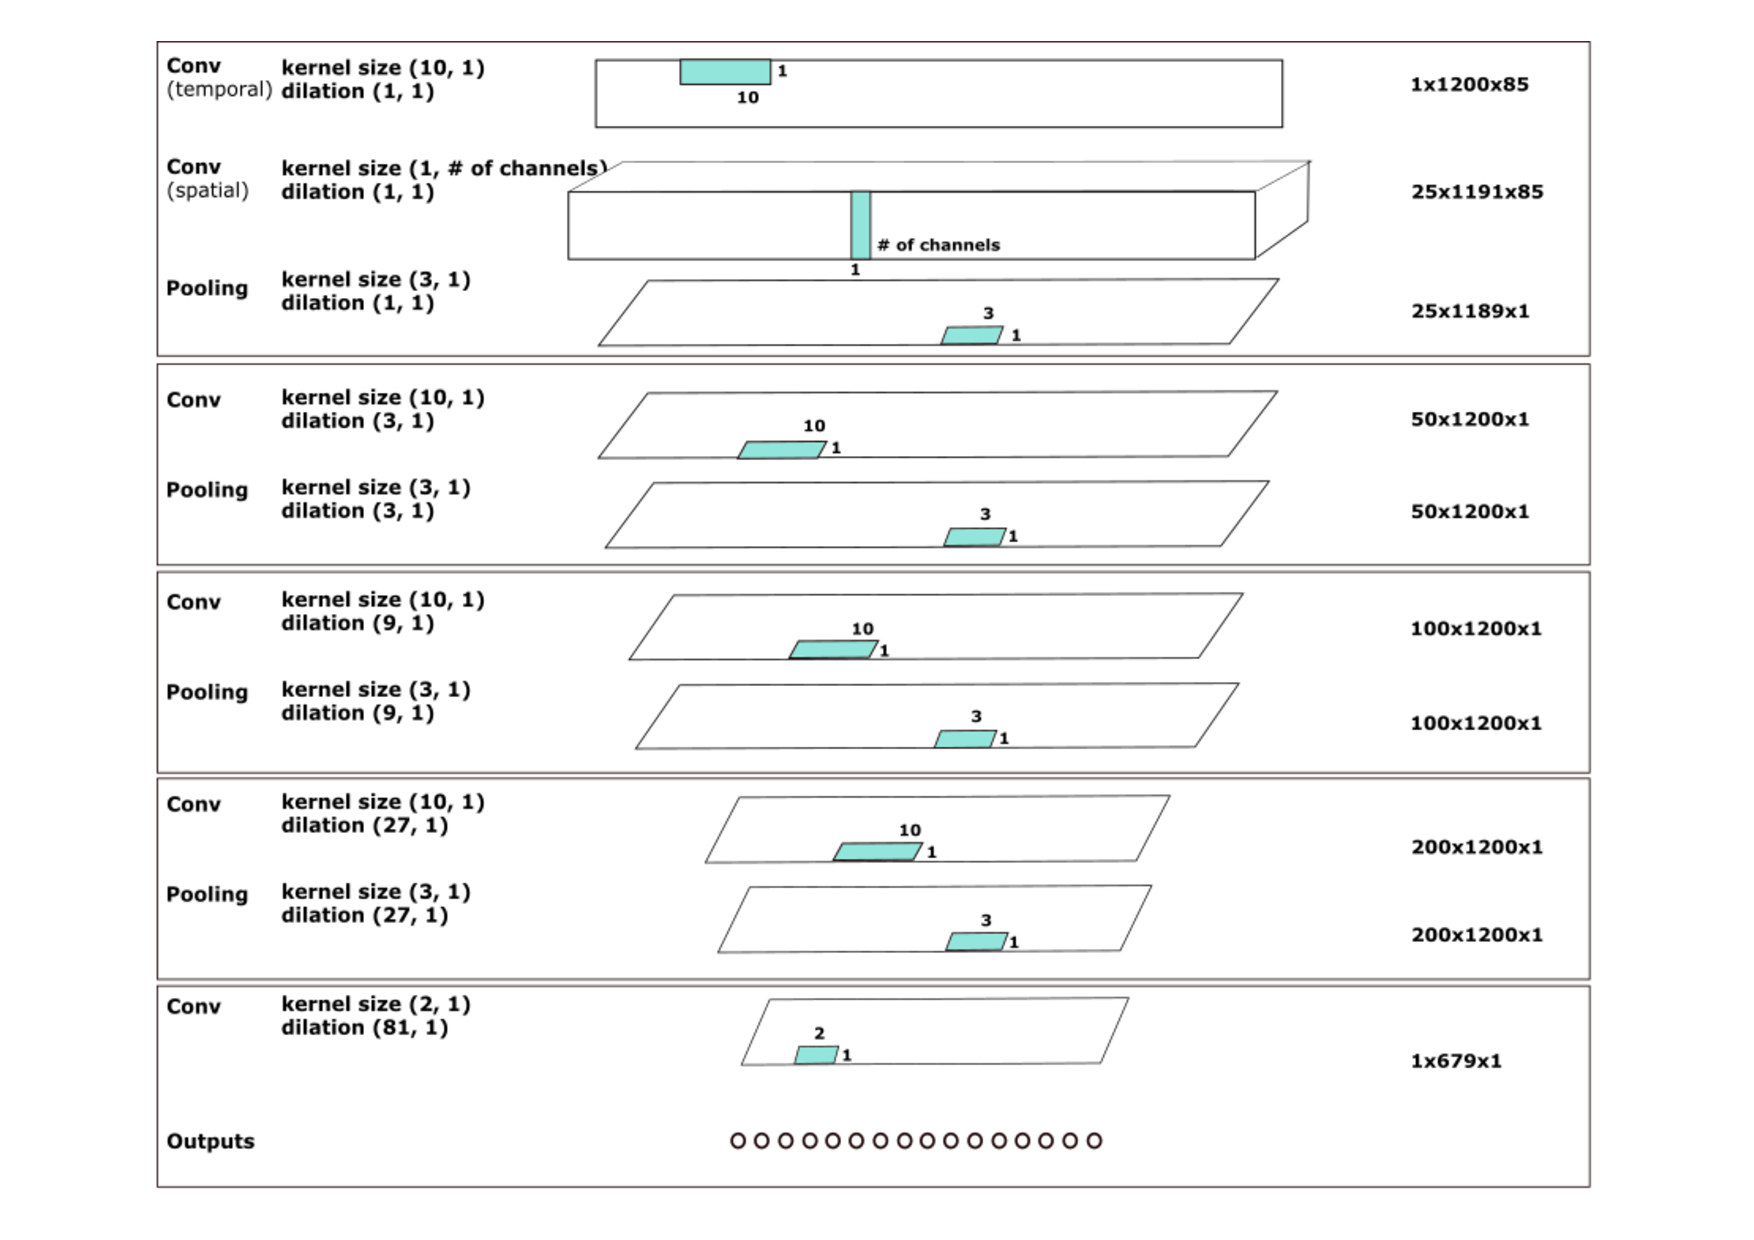
\includegraphics[width=\linewidth]{img/ch3/architektura}
\caption[Deep4Net architecture]{The architecture of the Deep4Net modified to be suitable for regression as used in~\cite{Hammer-2021} and in this thesis as k3\_d3\_sbp0.}
\label{fig:architecture}
\end{figure}

\subsection{Cropped decoding}\label{subsec:cropped-decoding}
The possibility to use cropped decoding is implemented the Braindecode library together with the original Deep4Net.
Cropped decoding allows, instead of obtaining one prediction per trial (Figure~\ref{fig:trial-wise-decoding-trial-wise}) to separate the trial window into multiple smaller overlapping sub-windows (crops) each of which produces a prediction (Figure~\ref{fig:trial-wise-decoding-cropped}).

\begin{figure}[!htbp]
\centering
\begin{subfigure}[a]{0.38\textwidth}
   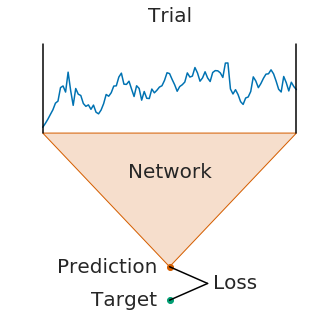
\includegraphics[width=\linewidth]{img/ch3/trialwise-explanation}
   \caption{Trial-wise decoding}
   \label{fig:trial-wise-decoding-trial-wise}
\end{subfigure}

\begin{subfigure}[b]{0.45\textwidth}
   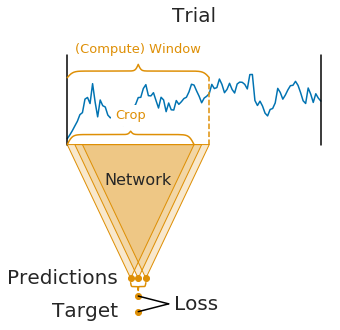
\includegraphics[width=\linewidth]{img/ch3/trialwise-explanation2}
   \caption{Cropped decoding}
   \label{fig:trial-wise-decoding-cropped}
\end{subfigure}
\caption[Trial-wise vs. cropped decoding]{This Figure obtained from the Braindecode library documentation\footnote{https://robintibor.github.io/braindecode/notebooks/Cropped\_Decoding.html} illustrates the difference between cropped decoding and trial-wise decoding for classification.}
\label{fig:trial-wise-decoding} 
\end{figure}

Cropped decoding can be implemented by processing one crop at a time.
But it can be sped up with dense prediction (discussed in Section~\ref{subsec:dilated-networks}) because every CNN\footnote{By every we mean standard CNN architecture similar to the Deep4Net consisting of convolution, pooling and batch-normalization layers.} which processes one crop at a time (one-crop network) and has no right padding can be transformed into a dilated network which simultaneously processes multiple crops and gives outputs equivalent to the one-crop network. 
A visual explanation of this is in Figure~\ref{fig:cropped-decoding-scheme}.


\begin{figure}[!htbp]
\centering
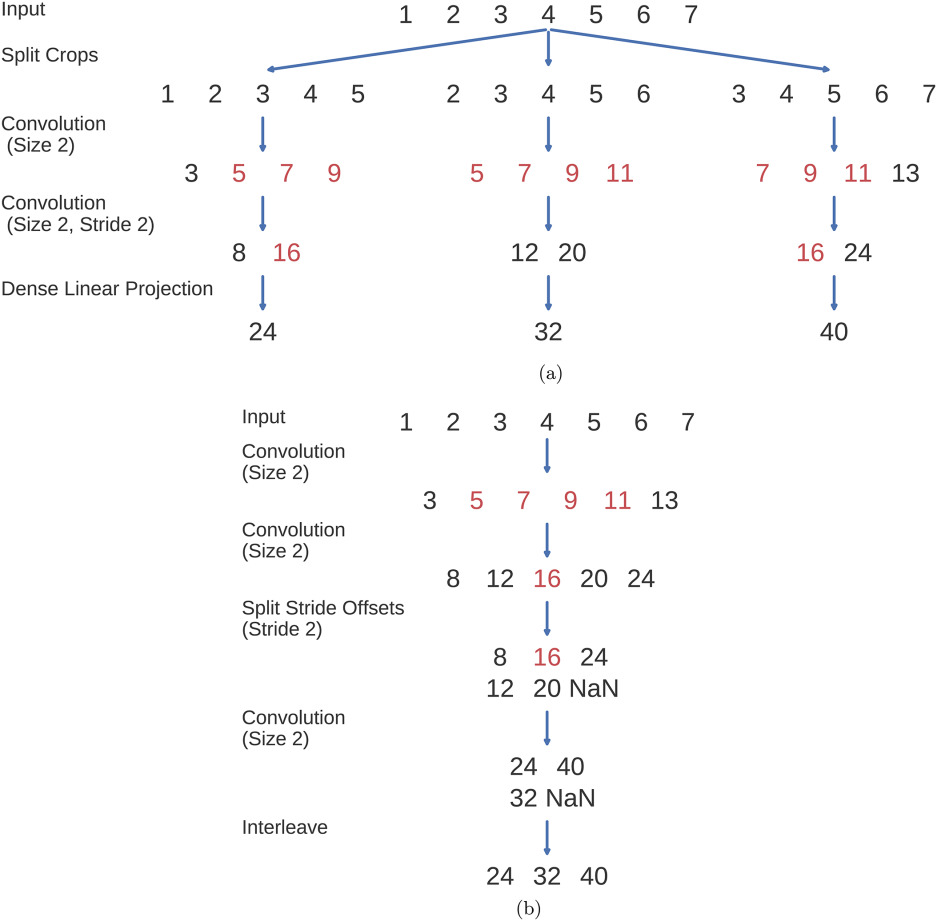
\includegraphics[width=\linewidth]{img/ch3/cropped-decoding-scheme}
\caption[Processing crops]{A toy example from~\cite{schirrmeister-deep-2017} presenting the difference between \textbf{a)} the naive approach to process crops using a network with strides; and \textbf{b)} processing multiple crops at the same time using the dilated network.}
\label{fig:cropped-decoding-scheme}
\end{figure}

The transformation of the one-crop network to the corresponding dilated network simply sets the strides in convolutional and max-pooling layers to one and replaces them with increased dilations.
The algorithm used to make the transition between strides and dilations is described in Algorithm\ref{alg:stride-to-dilation}. This algorithm allows us to transform every one-crop network without right padding into an equivalent dilated network.

Nevertheless, this transformation relationship is not symmetric.
For some dilated networks no one-crop network with strides (without right padding) exists.
An example of such a network is a CNN where in two consecutive layers with a dilation parameter, the first layer has bigger dilation than the second one.
This cannot happen if we follow Algorithm~\ref{alg:stride-to-dilation} thus, such a CNN was not derived from a one-crop network.

\begin{algorithm}
\begin{lstlisting}[language=Python,label={lst:lstlisting}]
def to_dense_prediction(network):
	current_stride = 1
	for module in network.modules:
		if hasattr(module, 'dilation'):
			module.dilation = current_stride
		if hasattr(module, 'stride'):
			current_stride *= module.stride
			module.stride = 1
\end{lstlisting}
\caption{The simplified algorithm used to transform a network with strides to a network with dilations in the Braindecode library.
This version assumes a 1D stride and dilation which is sufficient for our case as all the strides in the networks are 1D.
}
\label{alg:stride-to-dilation}
\end{algorithm}


In~\cite{schirrmeister-deep-2017} where the Deep4Net originated, the architectures were constructed as one-crop nets and were then converted into dilated networks.
This leaves a whole set of architectures unexplored.
Namely, those dilated networks which cannot be constructed from a one-crop network.
In this thesis, we use the dilated networks to obtain multiple values of kinematic variables from multiple crops processed at the same time. 
And because there is no reason for our task to consider one-crop networks first and then create dilated networks from them, we are free to explore these architectures.
And we do so in Section~\ref{sec:architectural-modifications}.

\subsection{Receptive field}\label{subsec:receptive-field}
The fact that the Deep4Net cannot have right padding in order to process multiple crops at the same time affects its receptive field.
By receptive field we mean the part of the input of the network which affects one specific output (in our case it corresponds to one crop from which one predicion is made).
In Figure~\ref{fig:receptive-field} we visualize the receptive field used to predict one time-point.
The figure illustrates how many times each input sample, and the values derived from it, are used in a forward pass through the CNN to obtain the specific prediction.
Note, that the receptive field in no way illustrates the weights of the network.

\begin{figure}[!htbp]
\centering
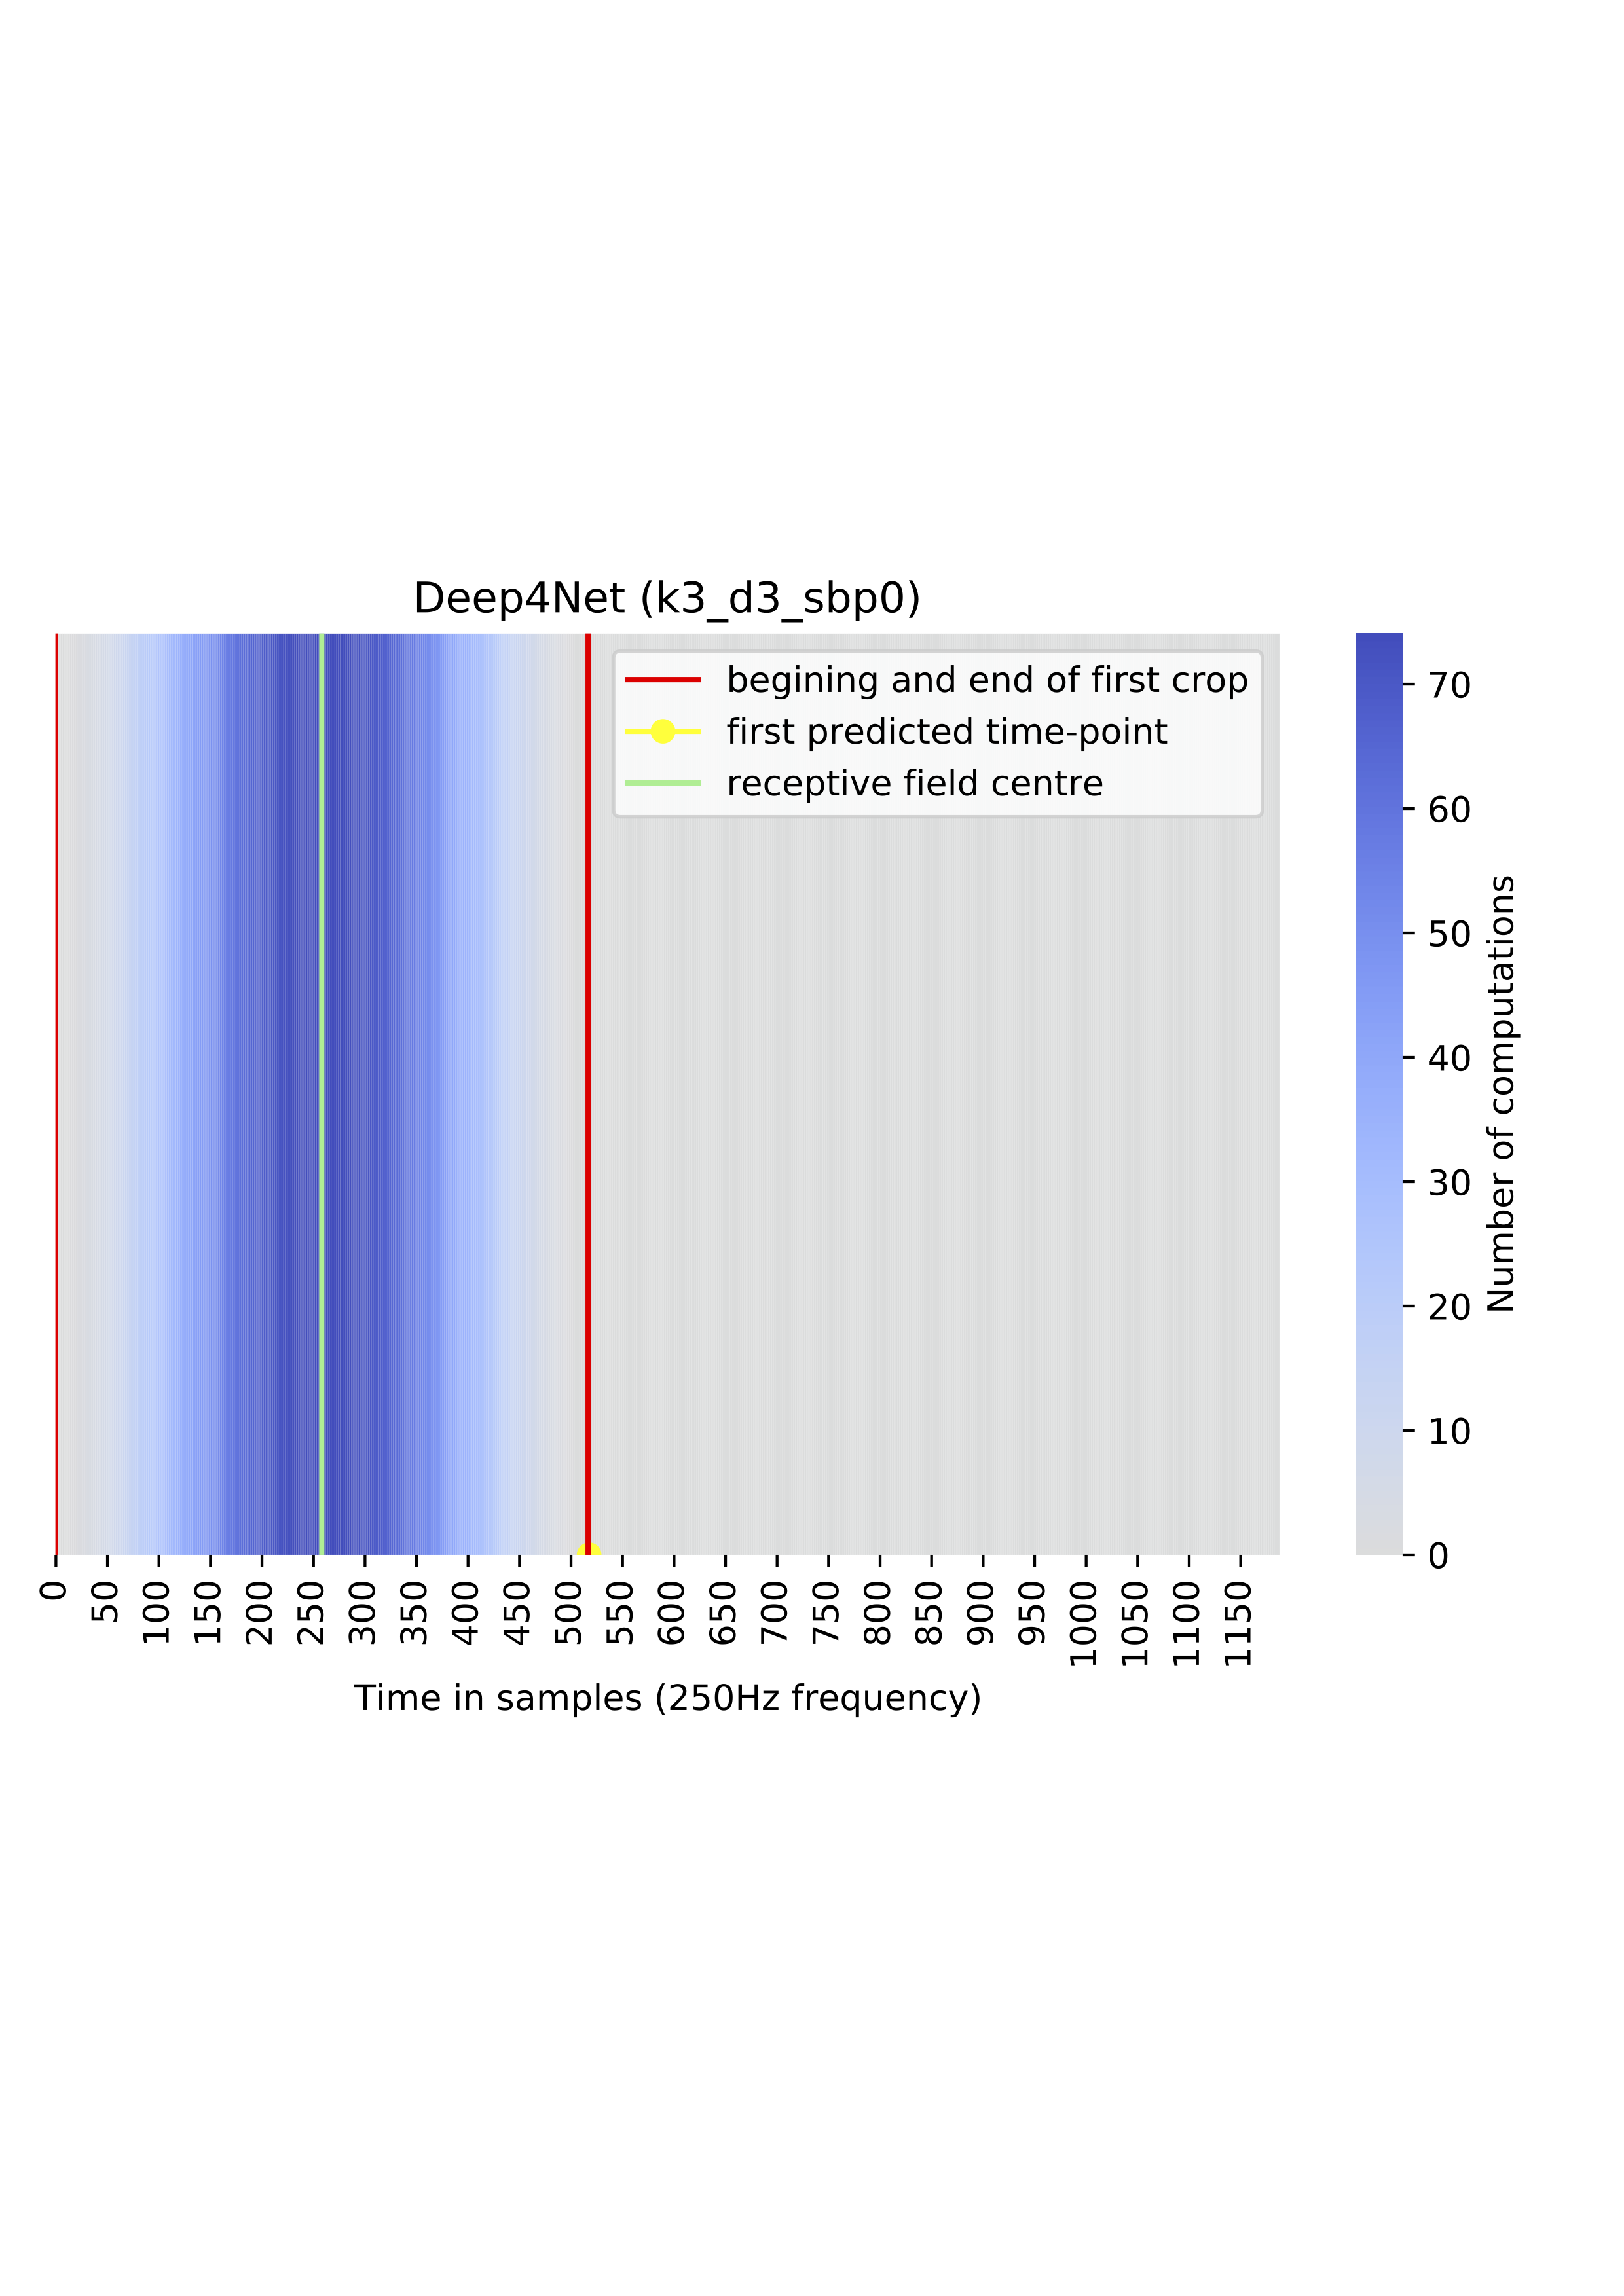
\includegraphics[width=0.8\linewidth]{img/ch3/deep4net-receptive-field}
\caption[Receptive field]{The receptive field of the original Deep4Net, which is the base model derived from~\cite{Hammer-2021}, in this thesis denoted as {variable}\_k3\_d3\_sbp0.
The vertical red lines delimit the receptive field (crop) of the CNN which is used for calculating the first prediction.
The whole gray area represents one input window.
The green line represents the centre of the receptive field and the yellow dot on the x axis the first time-point that is being predicted.
The gradient bar on the right shows the number of times each input sample was used in the calculations of the output.}
\label{fig:receptive-field}
\end{figure}

Figure~\ref{fig:receptive-field} illustrates that the predicted time-point is fairly far from the centre of the receptive field.
This is because we make the prediction only based on the data recorder prior to the predicted movement and do not use padding.
The CNN mostly focuses on signals around the centre of the receptive field and therefore, is biased towards data are far from those that directly precede the movement.

For classification this is not as critical, because the same label is predicted from multiple crops, and the actual classified movement does not happen at the end of the last crop but at some point during the whole input window from which the crops are derived (\cite{schirrmeister-deep-2017}).
This gives the network a chance to focus on information directly preceding the actual movement.

We focus on the changed role of the receptive field between classification and regression because as previously stated in~\cite{schirrmeister-deep-2017} and \cite{hartmann-hierarchical-2018}, this same CNN architecture was shown to utilize information from the high-gamma frequency bands.
Since we are investigating the frequency bands and their effective utilization, we inspect this difference as a possible reason for why the network, when employed to predict velocity and absolute velocity of hand movement, does not use high-gamma.
The hypothesis here is, that the high-gamma signal is most informative directly before the predicted movement execution.
Therefore, the distance of the network's receptive field centre to the predicted time-point hinders its usage.
We test this hypothesis in the \cref{sec:shifting-the-predicted-time-point}.

\subsection{Training}\label{subsec:training}
We left all hyper-parameters equal to those from~\cite{Hammer-2021}, because it was our goal to reproduce their results and build up on their research.
The only thing we changed was the learning rate.
The network was trained for 100 epochs with batch size 32, using the ADAM~ optimizer and learning rate 0.001.
The reported learning rate in \cite{Hammer-2021} was 0.01.
We used a lower learning rate because otherwise, the results were significantly worse than reported.

In~\cite{Hammer-2021} they performed leave-one-out cross-validation on the 25s-long segments.
Nevertheless, with the amount of different architecture and dataset modifications we explored, this would be extremely time-consuming.
A 5-fold cross-validation gave us a good estimation of the networks' performances while also saving computational power. 
To perform 5-fold-cross-validation we divided the 25s-long segments into 5 equal or almost equal subsets.
For each patient a separate 5-fold cross-validation was conducted.
The final performance was estimated from all 5 folds over each patient (see Section~\ref{subsec:performance-analysis}).


\subsection{Gradient visualization}\label{subsec:gradinet-visualization}
The gradient visualization algorithm is the following.
First, the input signal is converted into the power spectrum using Fourier transformation.
After this transformation, hooks are created for the amplitude and phase values.
Then it is converted back into the original signal, this time using the torch functions so PyTorch can start building its computational graph reaching back to the amplitudes and phases.
This tracked signal is then given to the network, whose weights are frozen, as input.
After obtaining the outputs, they are averaged and the \texttt{torch.autograd.backward()} function is used to derive the gradients with respect to the frequency amplitudes and phases (\cite{gradient-visualization}).

To obtain representative gradients, the above described procedure was always repeated over multiple batches for each patient and the resulting gradients were averages over the batches.
Gradients are useful in showing to modulations in which frequencies the network reacts more strongly.
The higher gradient value for a certain frequency, the more the change is this frequency influences the prediction.

Throughout the thesis, the input window size used in the above described algorithm was set to twice the size of the receptive field of the network to be consistent with~\cite{Hammer-2021}.
A special case is the gradient visualization when the input window is shortened so that the network has only one output was also briefly explored as a part of this thesis.
See section~\ref{sec:architectural-modifications}.
In this special case, the outputs did not have to be averaged before using the \texttt{torch.autograd.backward()} function to derive the gradients.
 
Because there are no significant differences between the gradients of the networks on the training set and the validation set we chose to always display the gradient values for the training set.
Also note that in this thesis we only address the gradients for the amplitudes of frequencies.
While inspecting the phase gradients would also be interesting, it is out of the scope of this thesis.

\subsection{Architectural modifications}\label{subsec:architectural-modifications}
During our research, we made a set of modifications to the architecture of the Deep4Net creating multiple new CNNs.
With our changes we focused on the kernel sizes and dilation parameters of the four max-pool layers present in the network.
Table~\ref{tab:architectures-description} explains the terminology used with respect to the changing max-pool parameters used throughout the thesis.
The original Deep4Net corresponds to the \{variable\}\_k3\_d3\_sbp0 in Table\ref{tab:architectures-description}.
The suffix \texttt{sbp} refers to a parameter of the Deep4Net, namely the \texttt{stride\_before\_pool} parameter.
This parameter influences the dilations in the max-pool layers of the network.
In~\cite{Hammer-2021} and~\cite{schirrmeister-deep-2017} this parameter was set to \texttt{False (sbp0)}.
The only analysis where the \texttt{stride\_before\_pool} was set to \texttt{True (sbp1)} was when analyzing a gradient peak (briefly discussed in Section~\ref{sec:architectural-modifications}) and also to study the dependence of the size of the receptive field on the performance of the network.
See Figure~\ref{fig:figure-distance}. \\

Therefore, we mention the Deep4Net with \texttt{sbp1} in Section~\ref{sec:architectural-modifications} but the default Deep4Net architecture is the one with \texttt{sbp0} as in~\cite{Hammer-2021} and~\cite{schirrmeister-deep-2017}.
We do not specify the \texttt{stride\_before\_pool} parameter for the other CNNs we created. It becomes meaningless because we manually set the sizes of the dilations for all the max-pool layers with no consideration of this parameter.

When we change the parameters of the max-pool layers as we describe above, the number of outputs of the network changes.
It also causes changes in the receptive field of the network.
To see how, consider just one max-pool layer with dilation 3 (L3) and one max-pool layer with dilation 1 (L1), both without padding.
If we use a window of the same length as input for L3 and L1 and compare the dimensions of the outputs from these layers, the dimension of the output of L3 will be smaller than of the L1.
\todo{illustration of this}
Consequently, if we alter the dilation (and also kernel size) parameters of the max-pool layers in the Deep4Net, we get a different number of outputs from the altered network.

When one network has dilations 3, 9, 27 and 81 in the max-pool layers (the k*\_d3) and the other one 1, 1, 1 and 1 (k*\_d1), the difference in the dimension of the output is significant.
The latter network makes more predictions from the same input window length because the dimension of the output is larger.
It also has a smaller receptive field for one prediction as is visualized in Figure~\ref{fig:receptive-field-comparison}.
Information about the size of the receptive field can be found in Table~\ref{tab:architectures-description}.

\begin{figure}[!htpb]
\centering
\begin{subfigure}[b]{0.44\textwidth}
   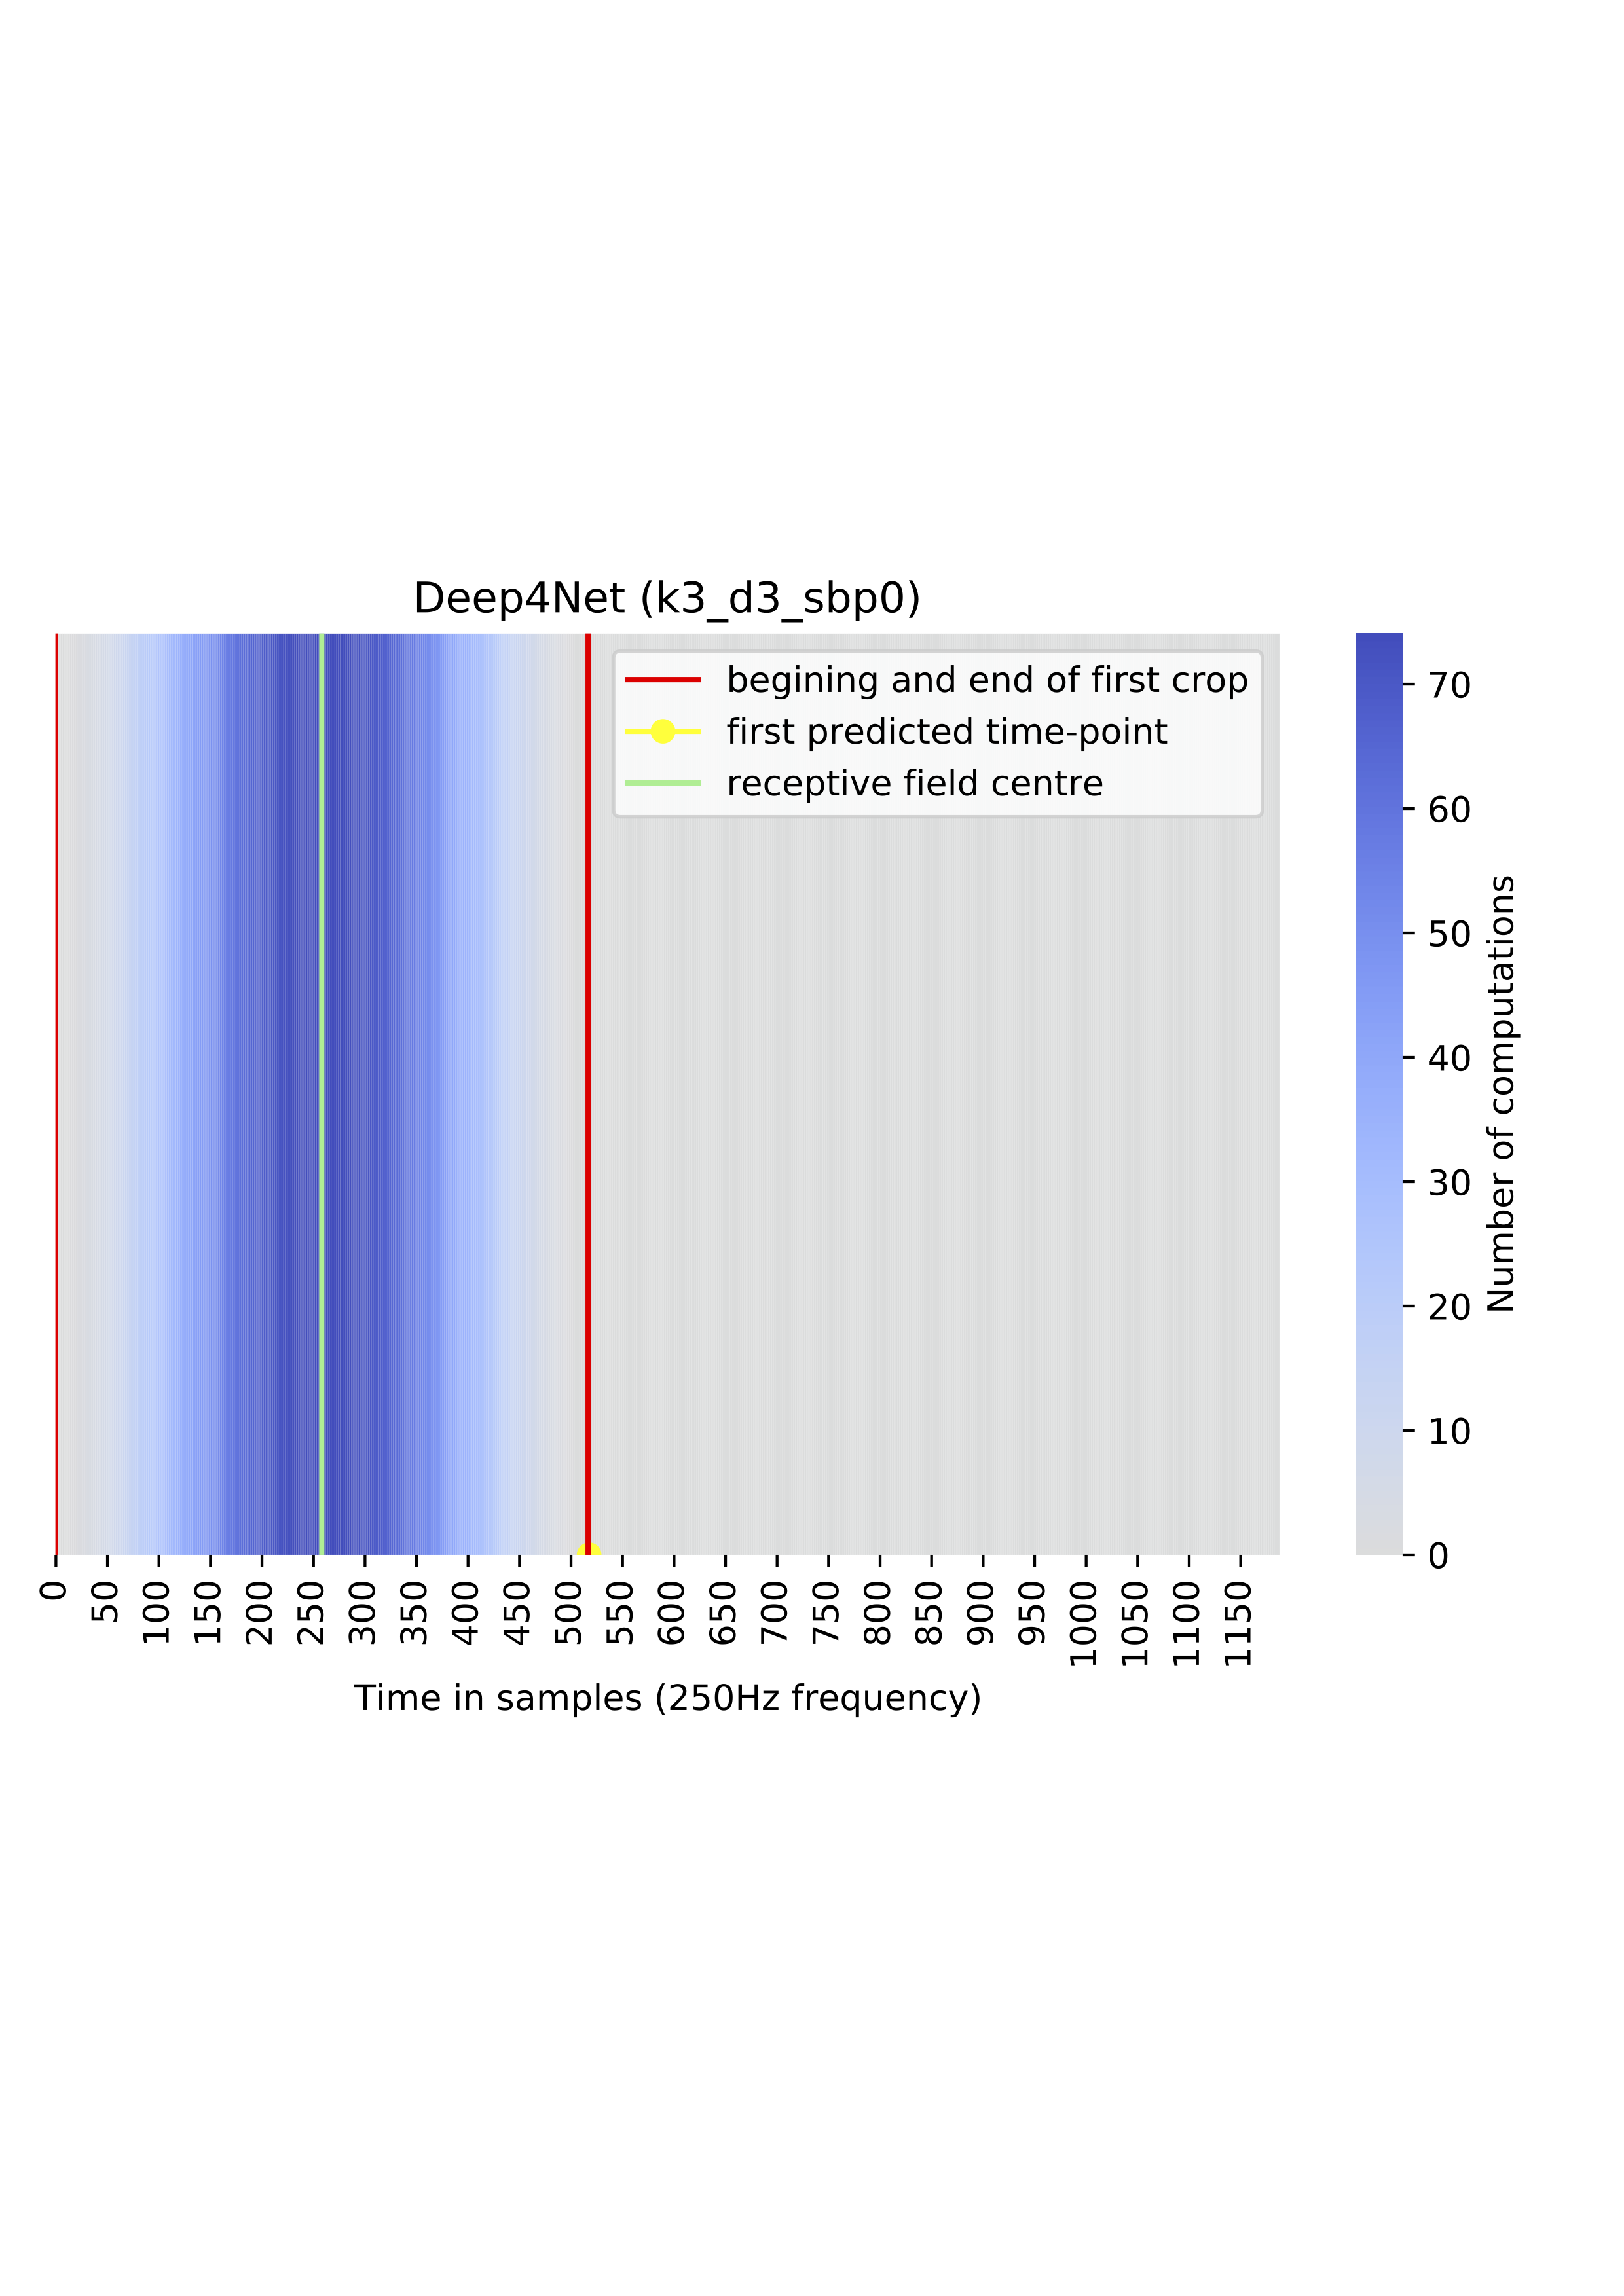
\includegraphics[width=\linewidth]{img/ch3/deep4net-receptive-field}
   \caption{Receptive field of the Deep4Net (k3\_d3\_sp0).}
\end{subfigure}
\begin{subfigure}[b]{0.44\textwidth}
   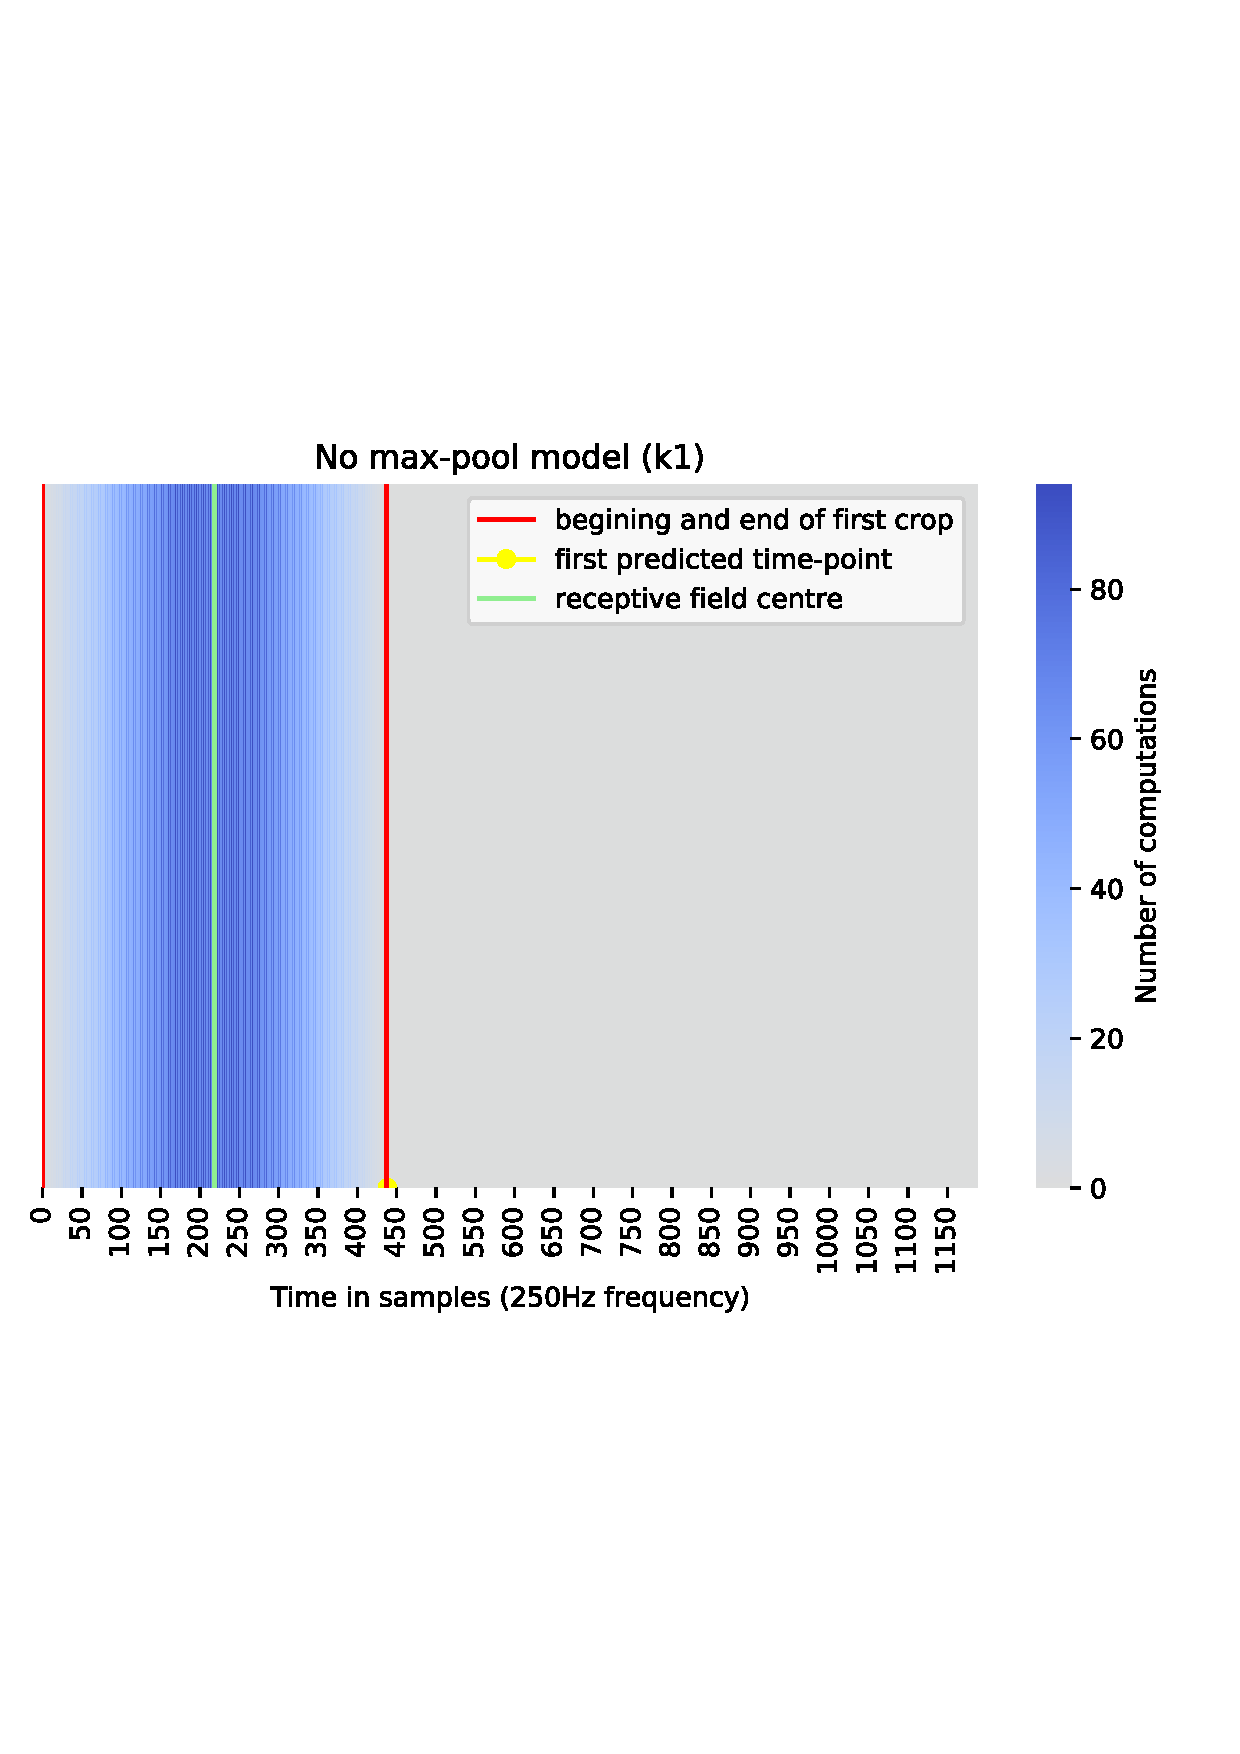
\includegraphics[width=\linewidth]{img/ch3/k1-receptive-field}
   \caption{Receptive field of the CNN without max-pool (k1).}
\end{subfigure}
\caption[Receptive field comparison]{Both graphs \textbf{(a)} and \textbf{(b)} show the receptive fields (delimited by red lines) used for predictig the first time-point (yellow dot on the x-axis).
The receptive field in \textbf{(b)} is smaller, reaching to less than 450, where as the receptive field of \textbf{(a)} reaches beyond 500.}
\label{fig:receptive-field-comparison}
\end{figure}

\begin{table}[!htpb]
\centering
\begin{tabular}{|p{3.7cm}|p{1.7cm}|p{2cm}|p{1.2cm}|p{2.5cm}|}
\toprule
Model name & Max-pool kernel size & Max-pool dilations & Stride before pool & Size of the receptive field \\
\midrule
variable\_k1 & 1, 1, 1, 1 & -- & -- & 442 samples \\
\hline
variable\_k2\_d3 & 2, 2, 2, 2 & 3, 9, 27, 81 & -- & 562 samples \\
\hline
variable\_k3\_d3\_sbp1 & 3, 3, 3, 3 & 3, 9, 27, 81 & True & 682 samples \\
\hline
variable\_k3\_d3\_spb0 & 3, 3, 3, 3  & 1, 3, 9, 27 & False & 522 samples \\
\hline
variable\_k2\_d1 & 2, 2, 2, 2 & 1, 1, 1, 1 & -- & 446 samples \\
\hline
variable\_k3\_d1 & 3, 3, 3, 3  & 1, 1, 1, 1 & -- & 450 samples \\
\hline
variable\_k2\_d2 & 2, 2, 2, 2 & 2, 4, 8, 16 & -- & 472 samples \\
\hline
variable\_k3\_d2 & 3, 3, 3, 3 & 2, 4, 8, 16 & -- & 502 samples \\
\hline
\bottomrule
\end{tabular}
\caption[Architectural modifications]{This table gives an overview of the various CNN architectures we investigated in the scope of this thesis.
Modifications were always made to the max-pooling layers.
Only information about the first dimension of the kernel sizes and dilations is presented.
The second dimension is always 1.
I.e. max-pool kernel sizes 2, 2, 2, 2 actually represent kernel sizes (2, 1), (2, 1), (2, 1), (2, 1). }
\label{tab:architectures-description}
\end{table}

\subsection{Performance analysis}\label{subsec:performance-analysis}
When comparing two CNNs, we are not comparing them based on the mean-square error (MSE) which is the loss function of the training, but on the correlation coefficient (CC) between the model's predictions and the predicted kinematic variable.
Specifically the Pearson's correlation coefficient~(\cite{pearson-vii-1895}).
Often throughout the thesis we show boxplots of CCs of different architectures.
Each boxplot is obtained from performing a 5-fold cross-validation for each of the 12 participants.
The results from the 5 folds are averaged and the box-plot is created from the 12 averages.
While it is possible to create the box-plots from all the folds, not averaging them for each patient, we are interested in the distribution of correlation among patients rather than among individual runs.
\chapter{Experiments and results}
\label{ch:exp}

\section{Gradient peak}\label{sec:gradient-peak}
As stated before, the input perturbation, output-correlation method in~\cite{Hammer-2021} did not point to high-gamma frequency amplitude as being strikingly important to the network. The gradient visualization also did not show particularly high gradients in the high-gamma band, unless the input window for the network was shortened so that the network had only one output, i.e. predicted one time-point. Two interesting observations could be made for the one-output gradient visualization:
\begin{itemize}
\item[1.] A gradient peak occurs at 83.88 Hz in both the untrained and the trained network and it is amplified with training.
\item[2.] If we add noise of a certain frequency or white noise to the input, frequencies around 83.33 Hz increases in the output of the network.
\end{itemize}

83.33Hz seems like a random frequency to have such a sharp peak in the frequency and also does not seem to be caused by a physiological property of the input signal.
A hypothesis was that the 83.33 Hz peak occurs due to this frequency being aligned with the dilations of the max-pool layers and therefore is just an architecture artifact.
Because sampling rate is 250 Hz and the dilations of the max-pool layers are powers of three and $250 Hz / 3 = 83.33 Hz$, this frequency aligns with the dilations of the max-pool layers which amplify it.
However, this does not explain why the peak at 83.33Hz is amplified with training.

To test the artifact hypothesis, we systematically changed the dilations of the max-pool layers to powers of 1, 2 and 3 and kernel sizes to 1\footnote{Importantly, when all max-pool layers in a network have their kernel size set to 1, it is equivalent to a network without max-pool layers.}, 2, 3 and 4

The results in Figure~\ref{fig:gradient-peak} demonstrate that the kernel size change has no effect on the 83.33Hz peak.
However, with change in the dilations, the 83.33 Hz peak disappears without a decrease in performance.
Another interesting thing to notice is to observe how the gradients of motor, non-motor and all channels behave with respect to each other.
The biggest differences between the gradients are in the alpha and beta bend where the motor gradients have visibly higher values than non-motor and all channels.
For the gradient peak at 83.33 Hz, the values of the motor, non-motor and all channels are almost equivalent.

\begin{figure}
\begin{subfigure}{.5\textwidth}
  \centering
  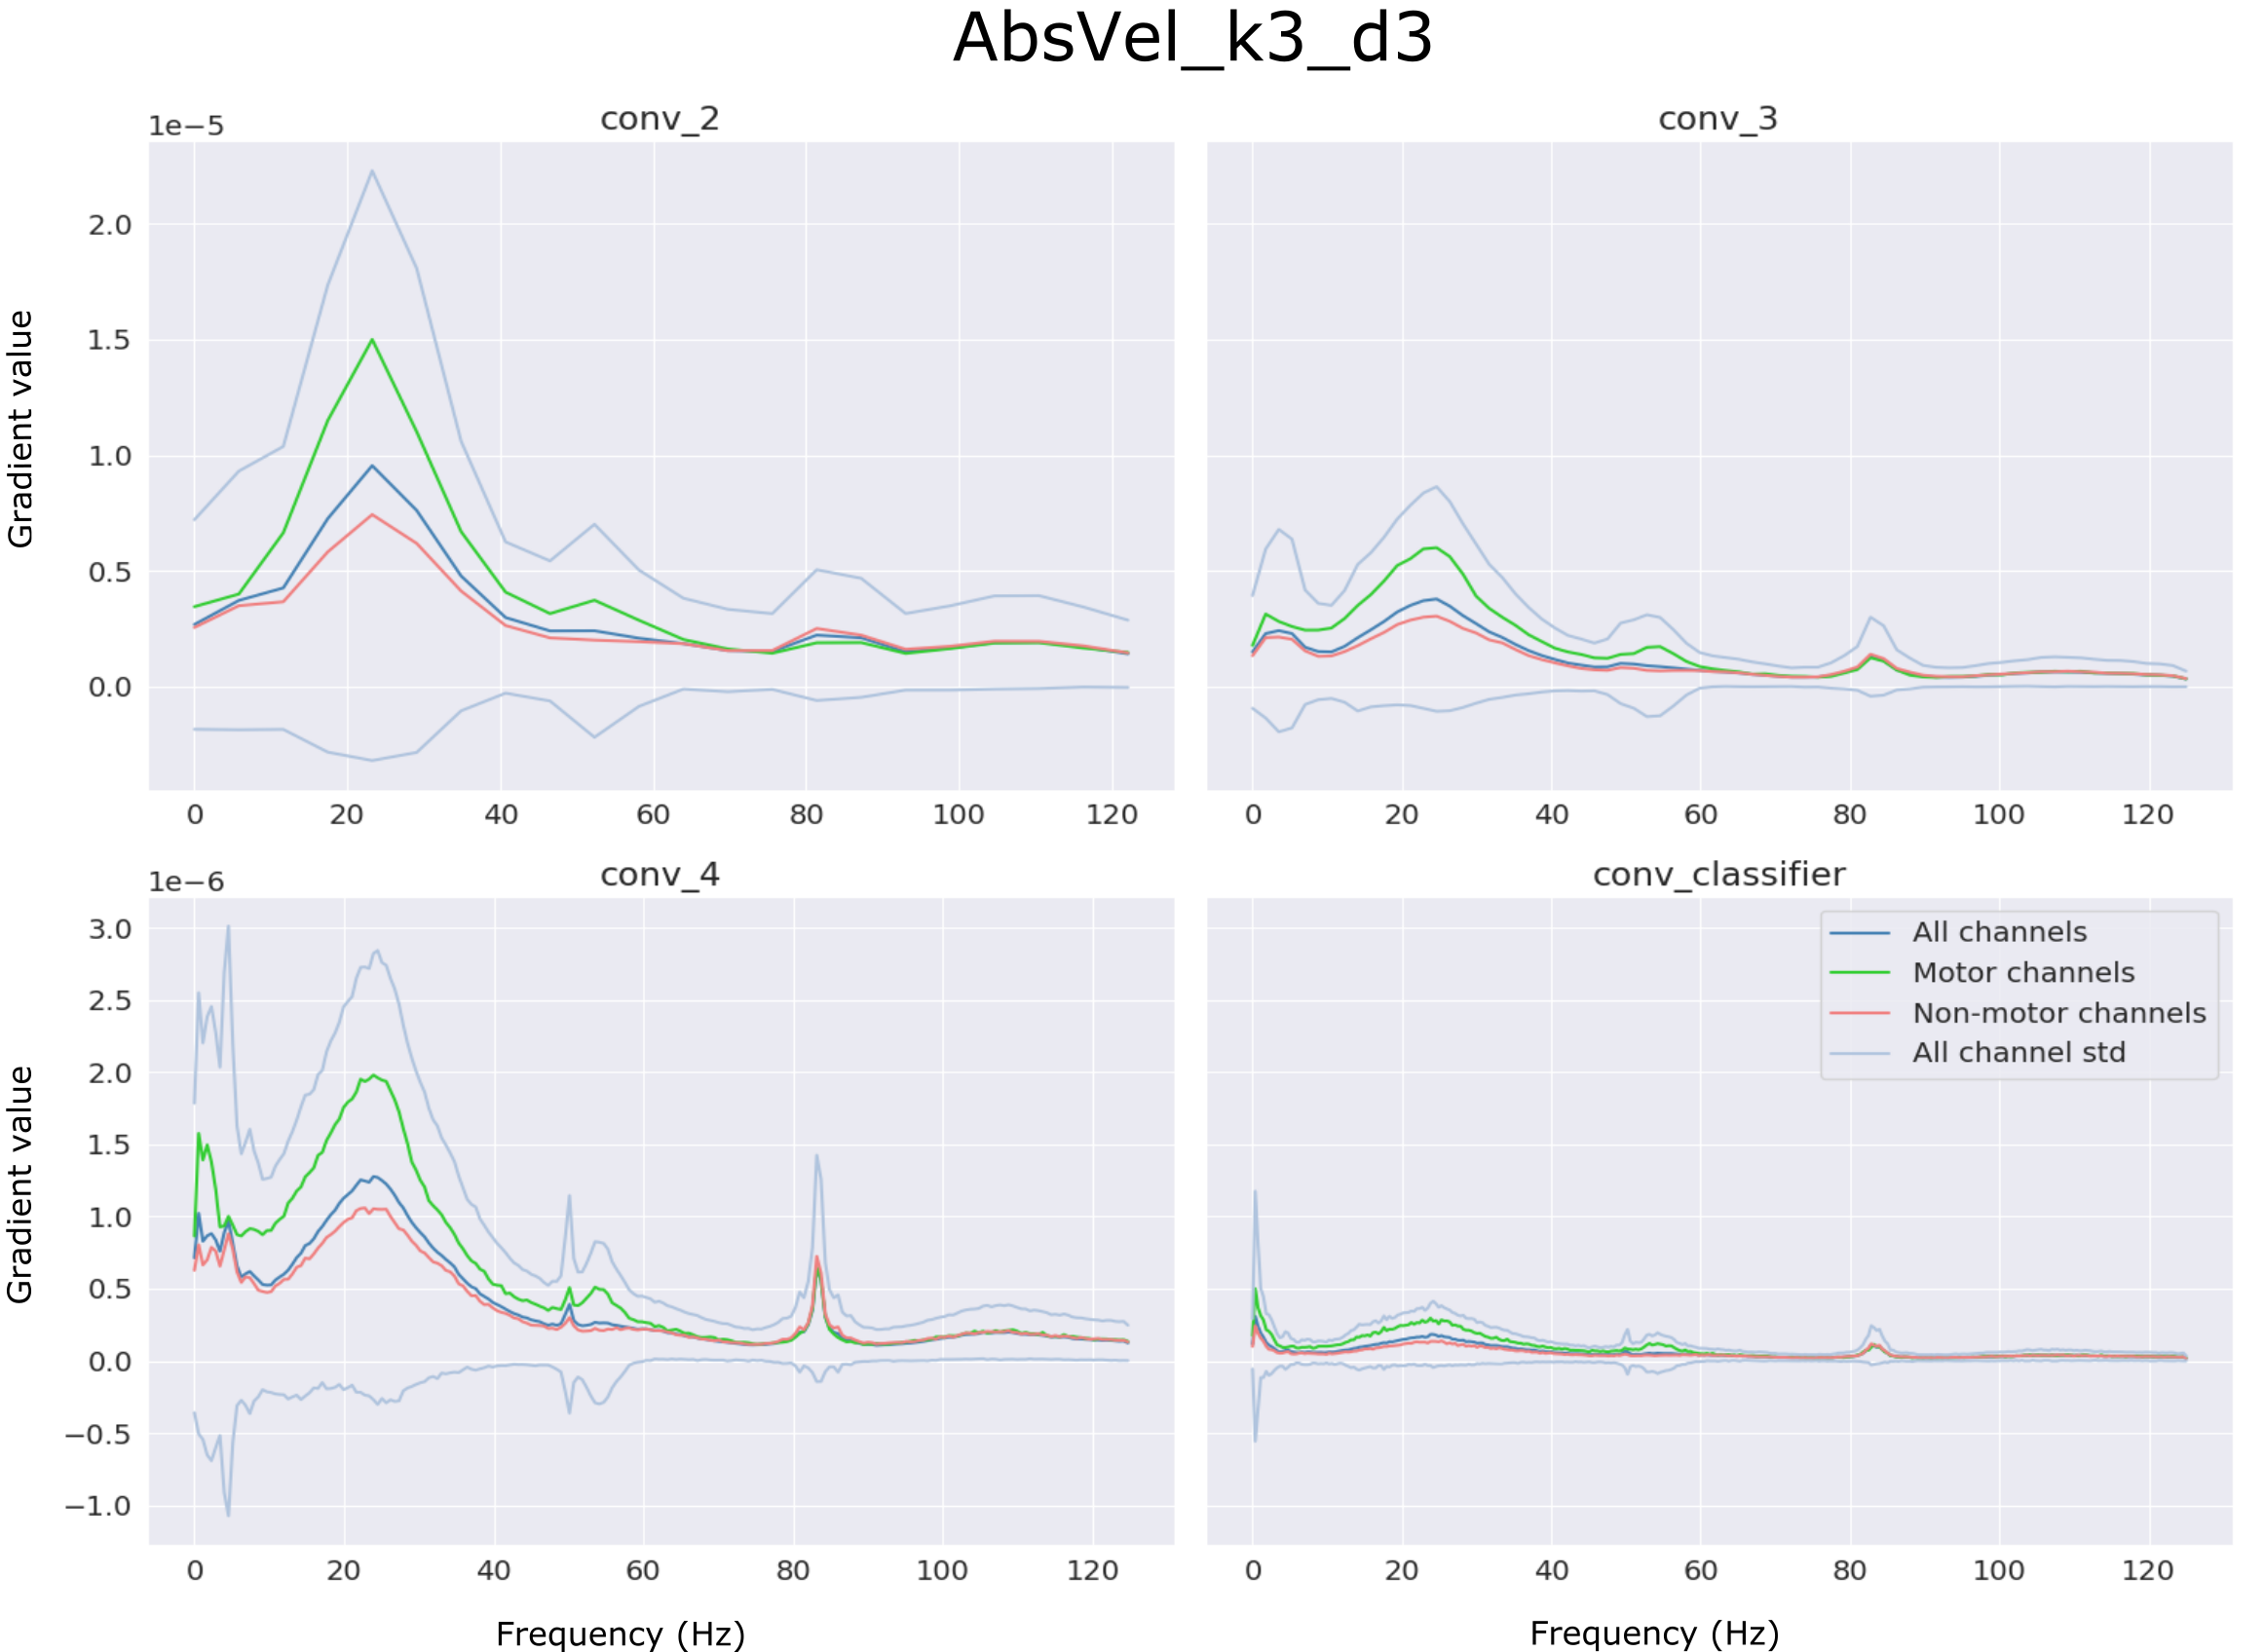
\includegraphics[width=.8\linewidth]{img/ch4/absVel-k3-d3}
  \caption{1a}
  \label{fig:absVel-k3-d3}
\end{subfigure}%
\begin{subfigure}{.5\textwidth}
  \centering
  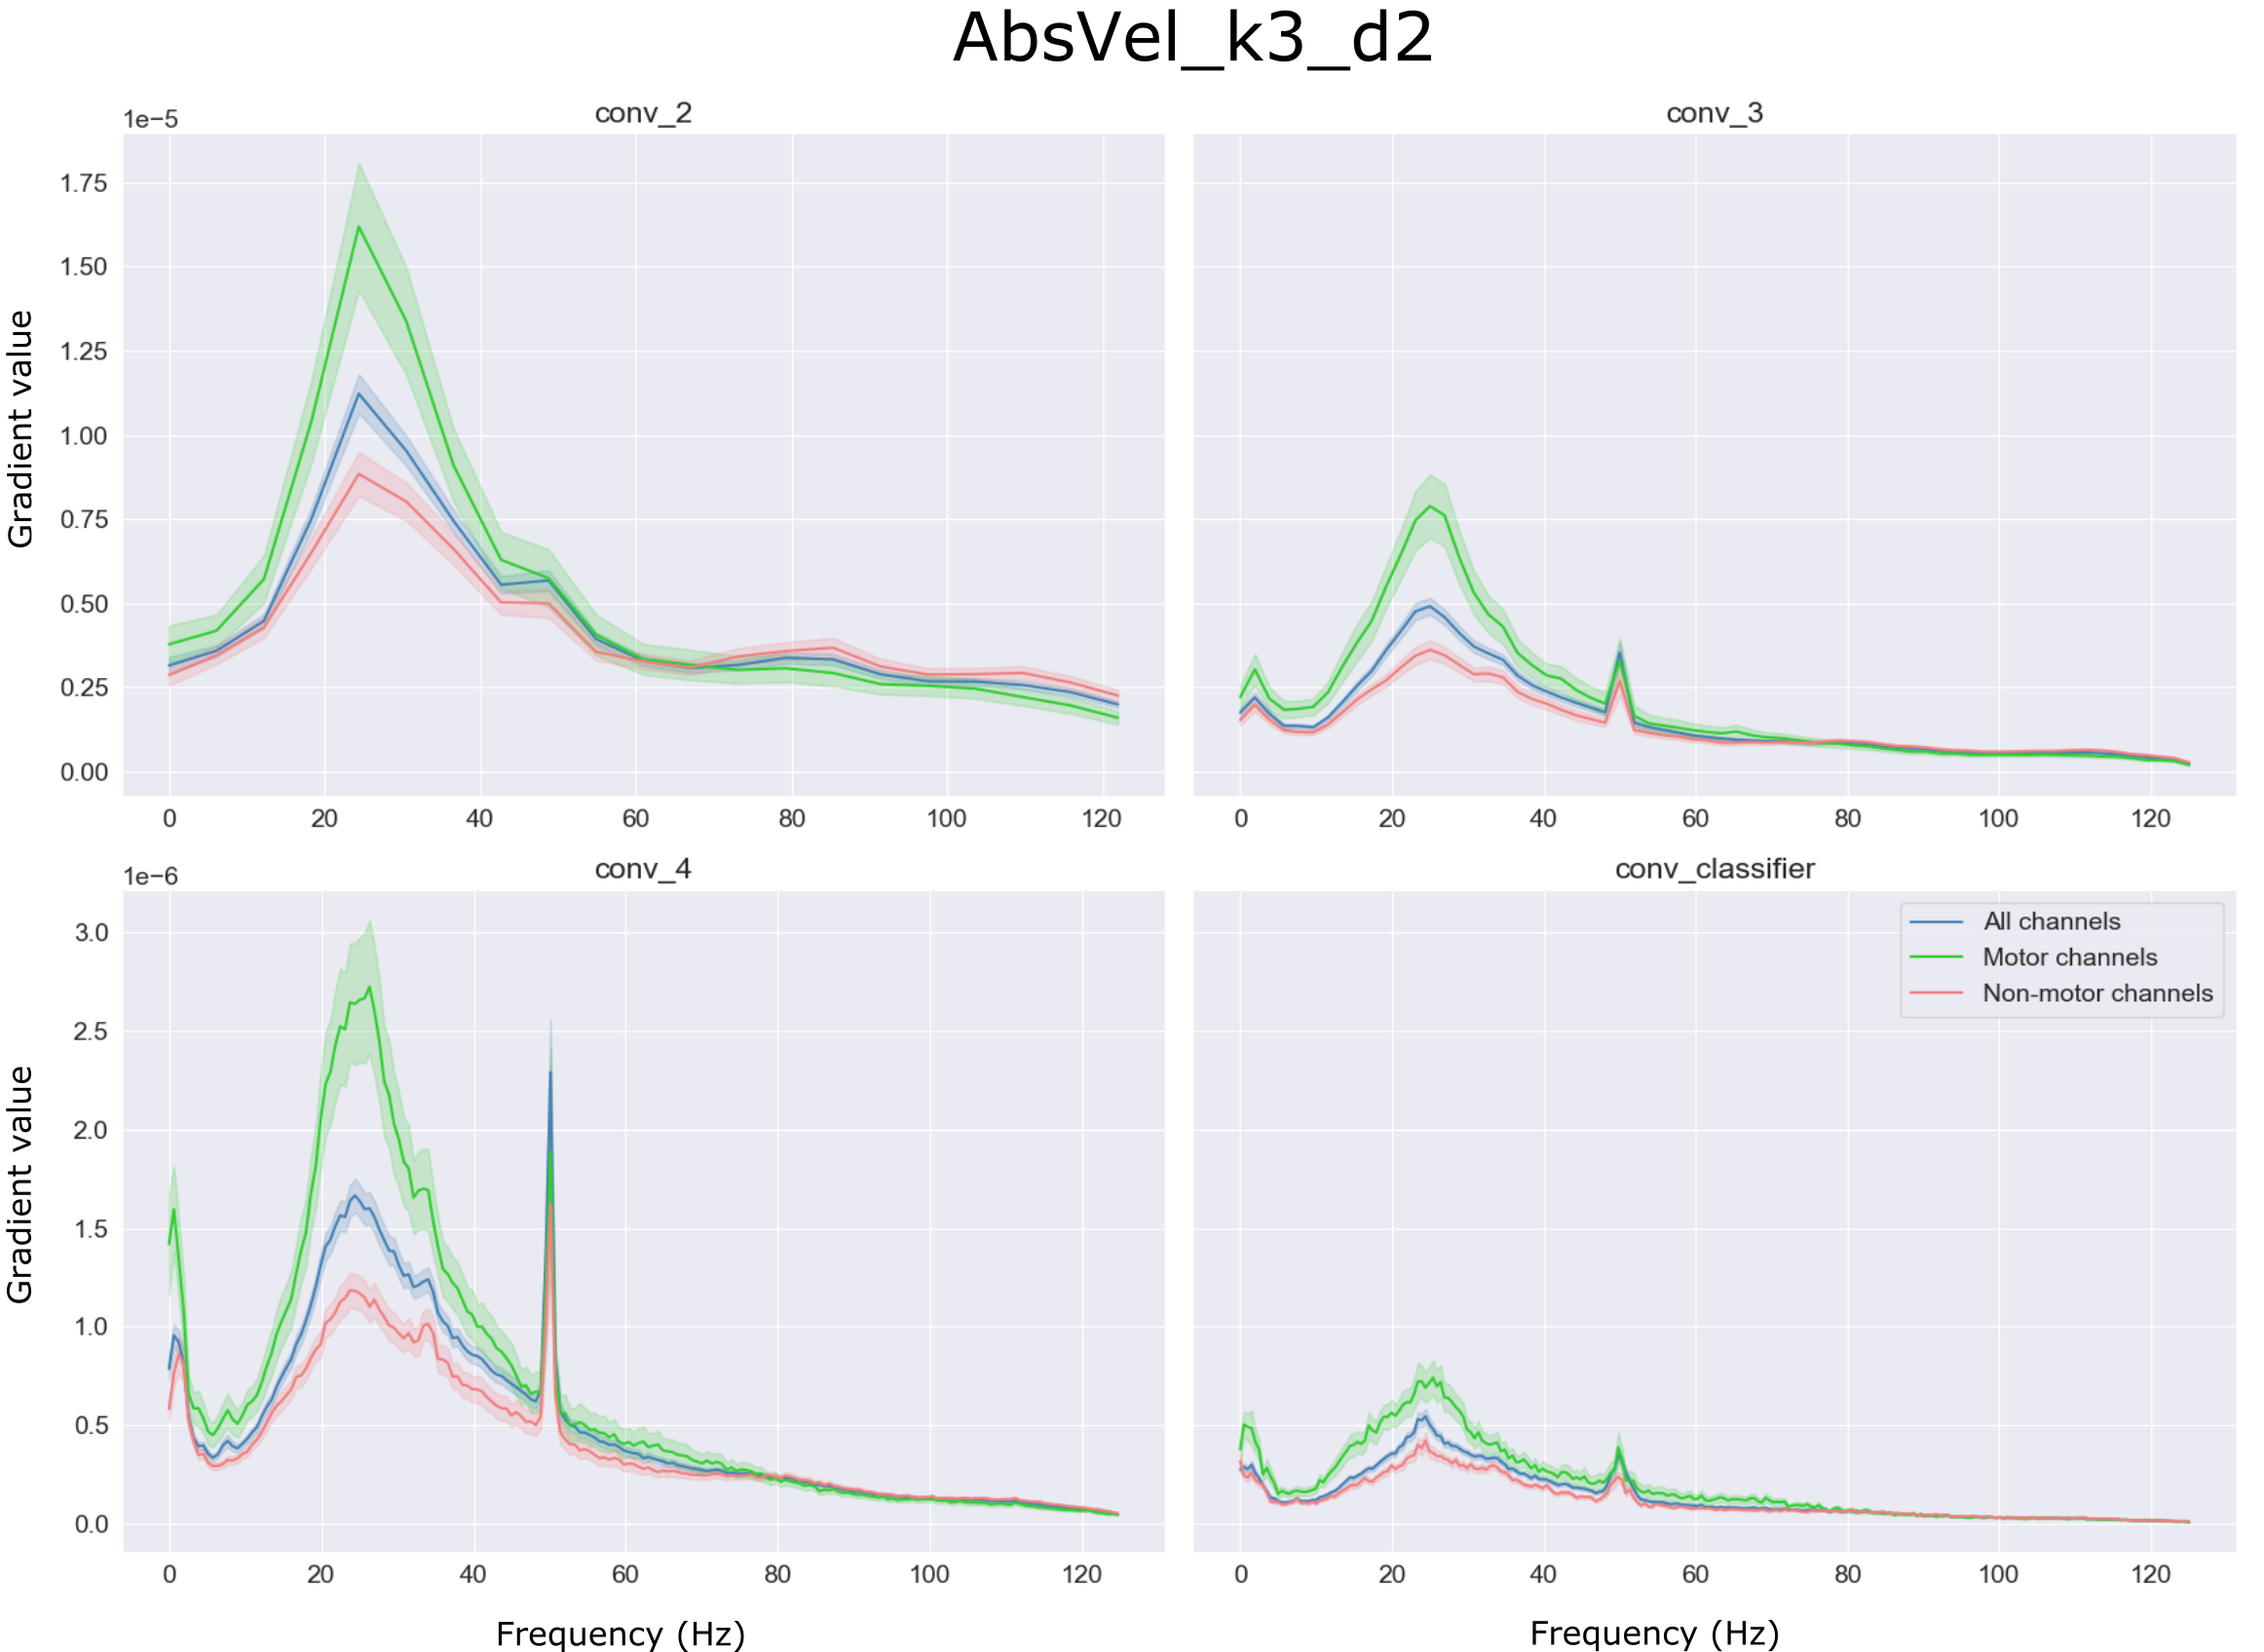
\includegraphics[width=.8\linewidth]{img/ch4/absVel-k3-d2}
  \caption{1b}
  \label{fig:absVel-k3-d2}
\end{subfigure}
\begin{subfigure}{.5\textwidth}
  \centering
  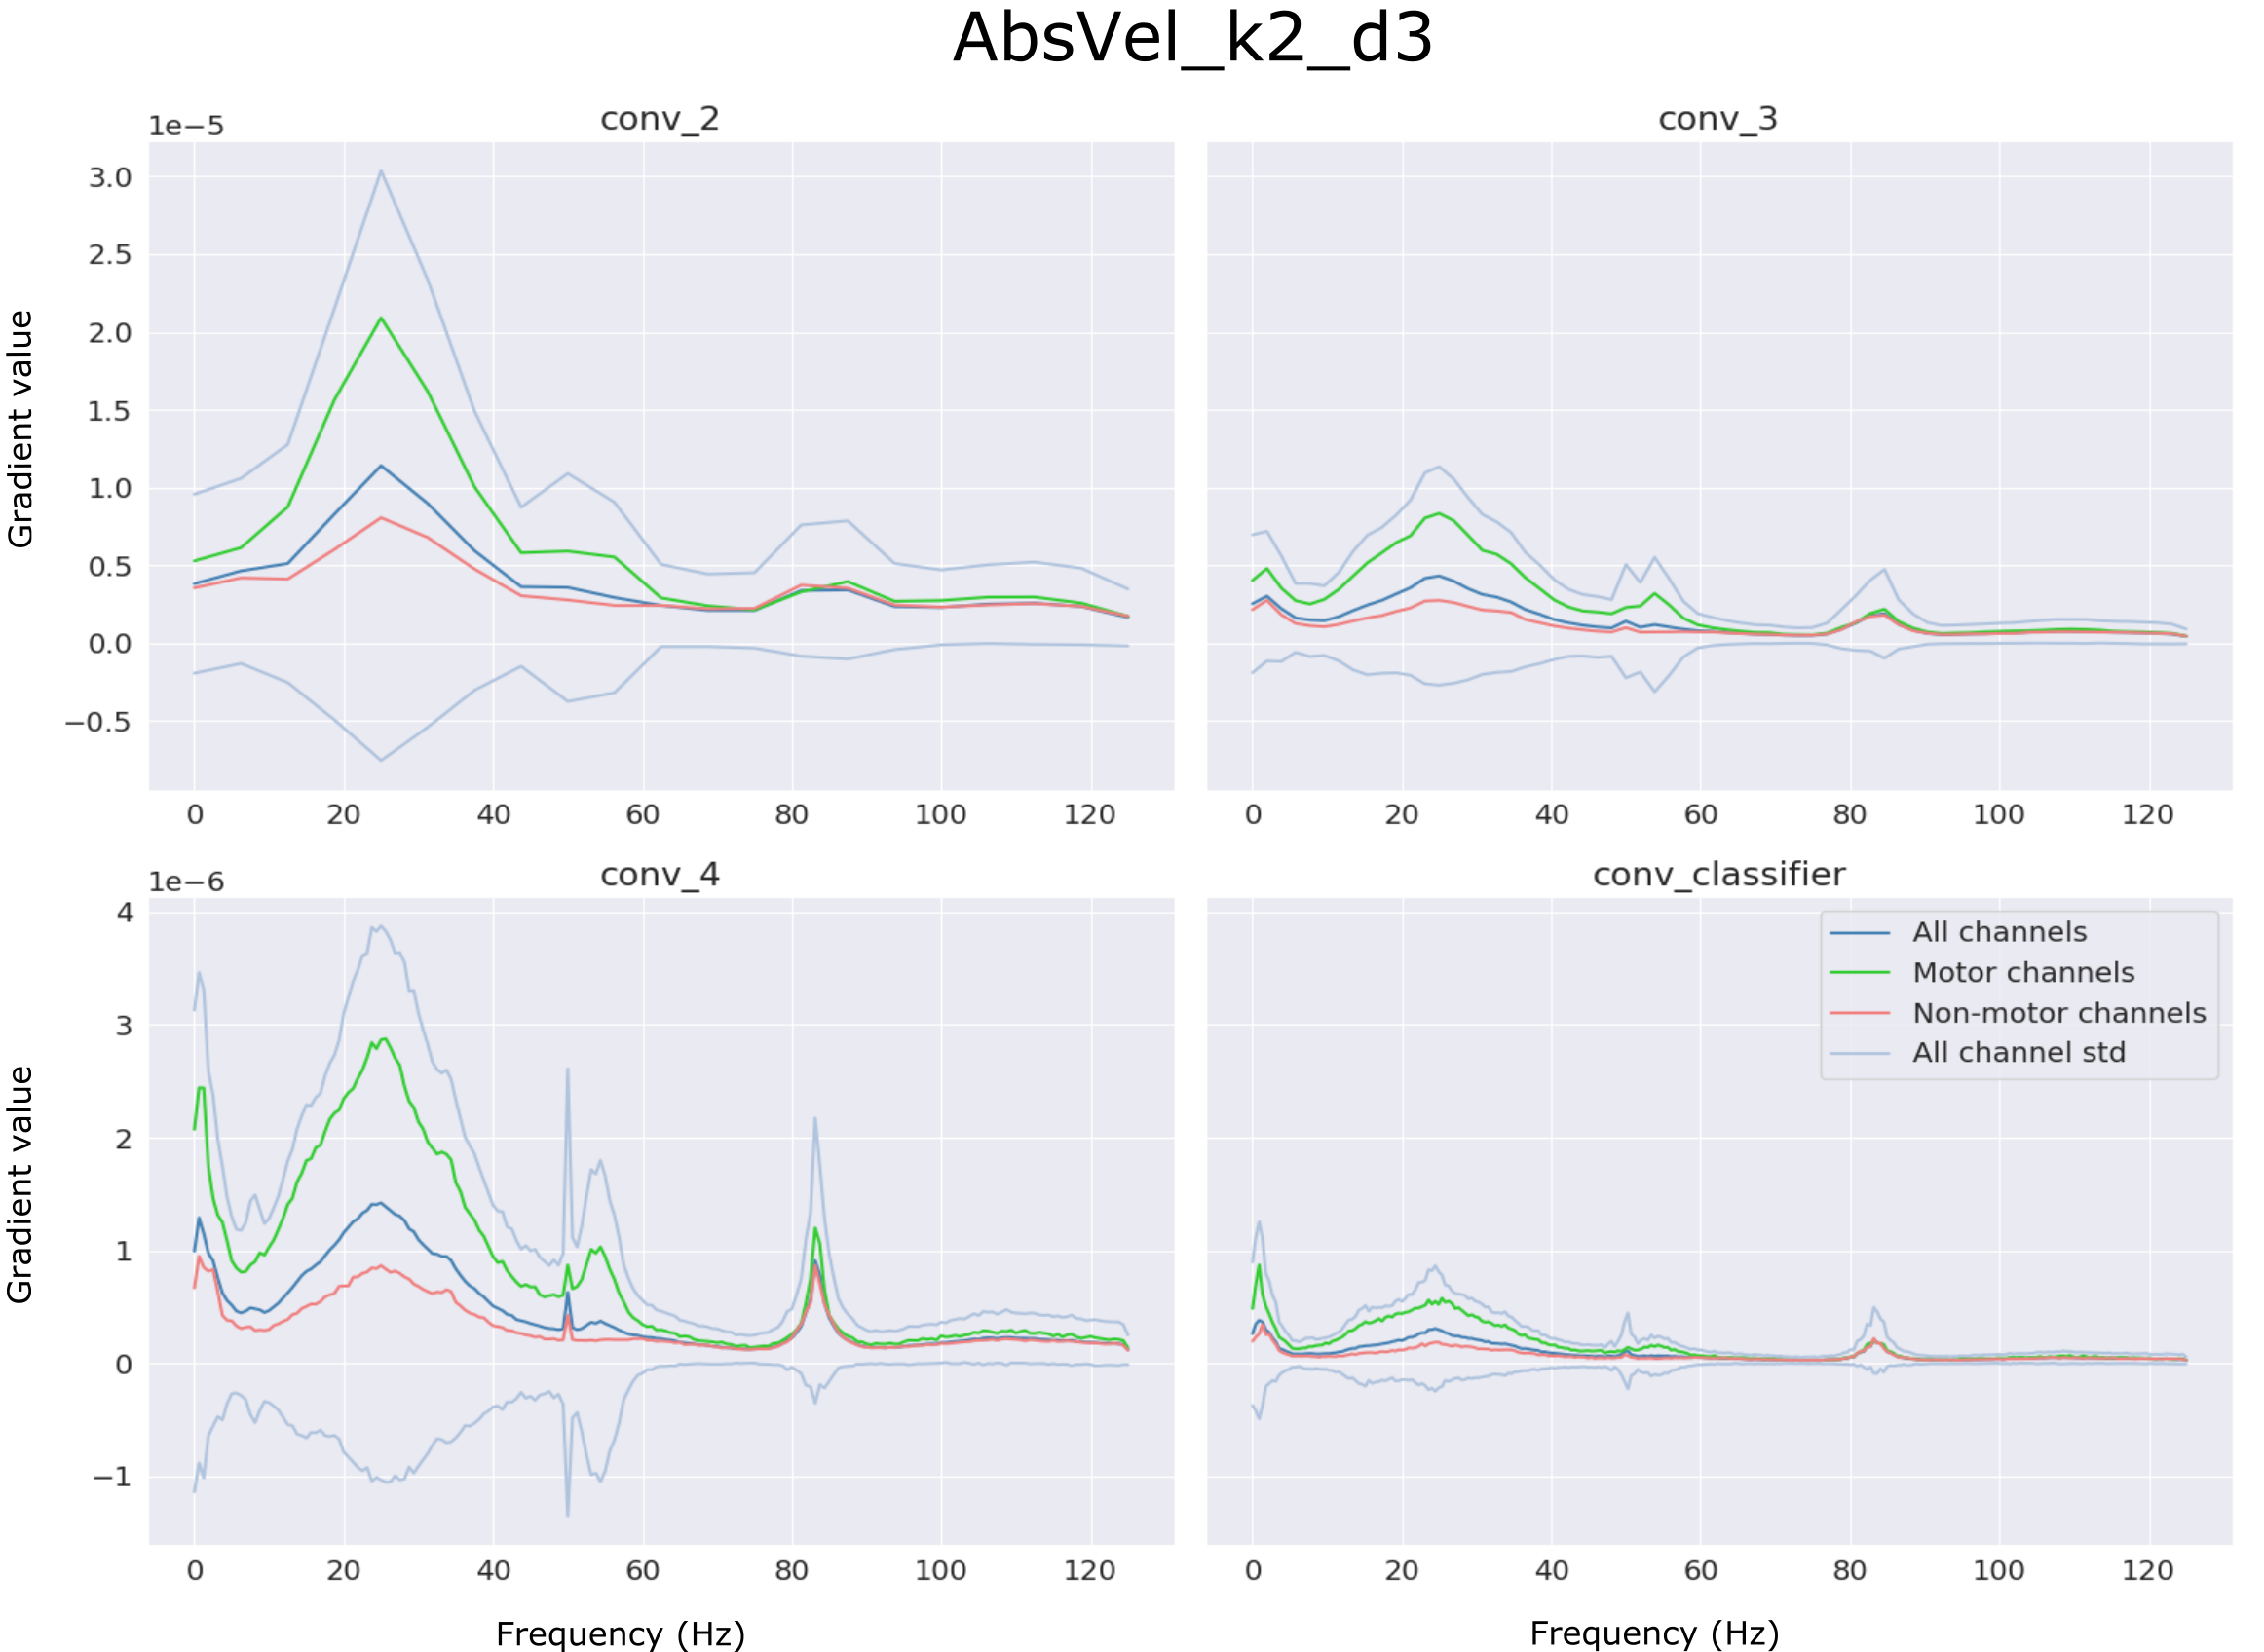
\includegraphics[width=.8\linewidth]{img/ch4/absVel-k2-d3}
  \caption{1a}
  \label{fig:absVel-k2-d3}
\end{subfigure}%
\begin{subfigure}{.5\textwidth}
  \centering
  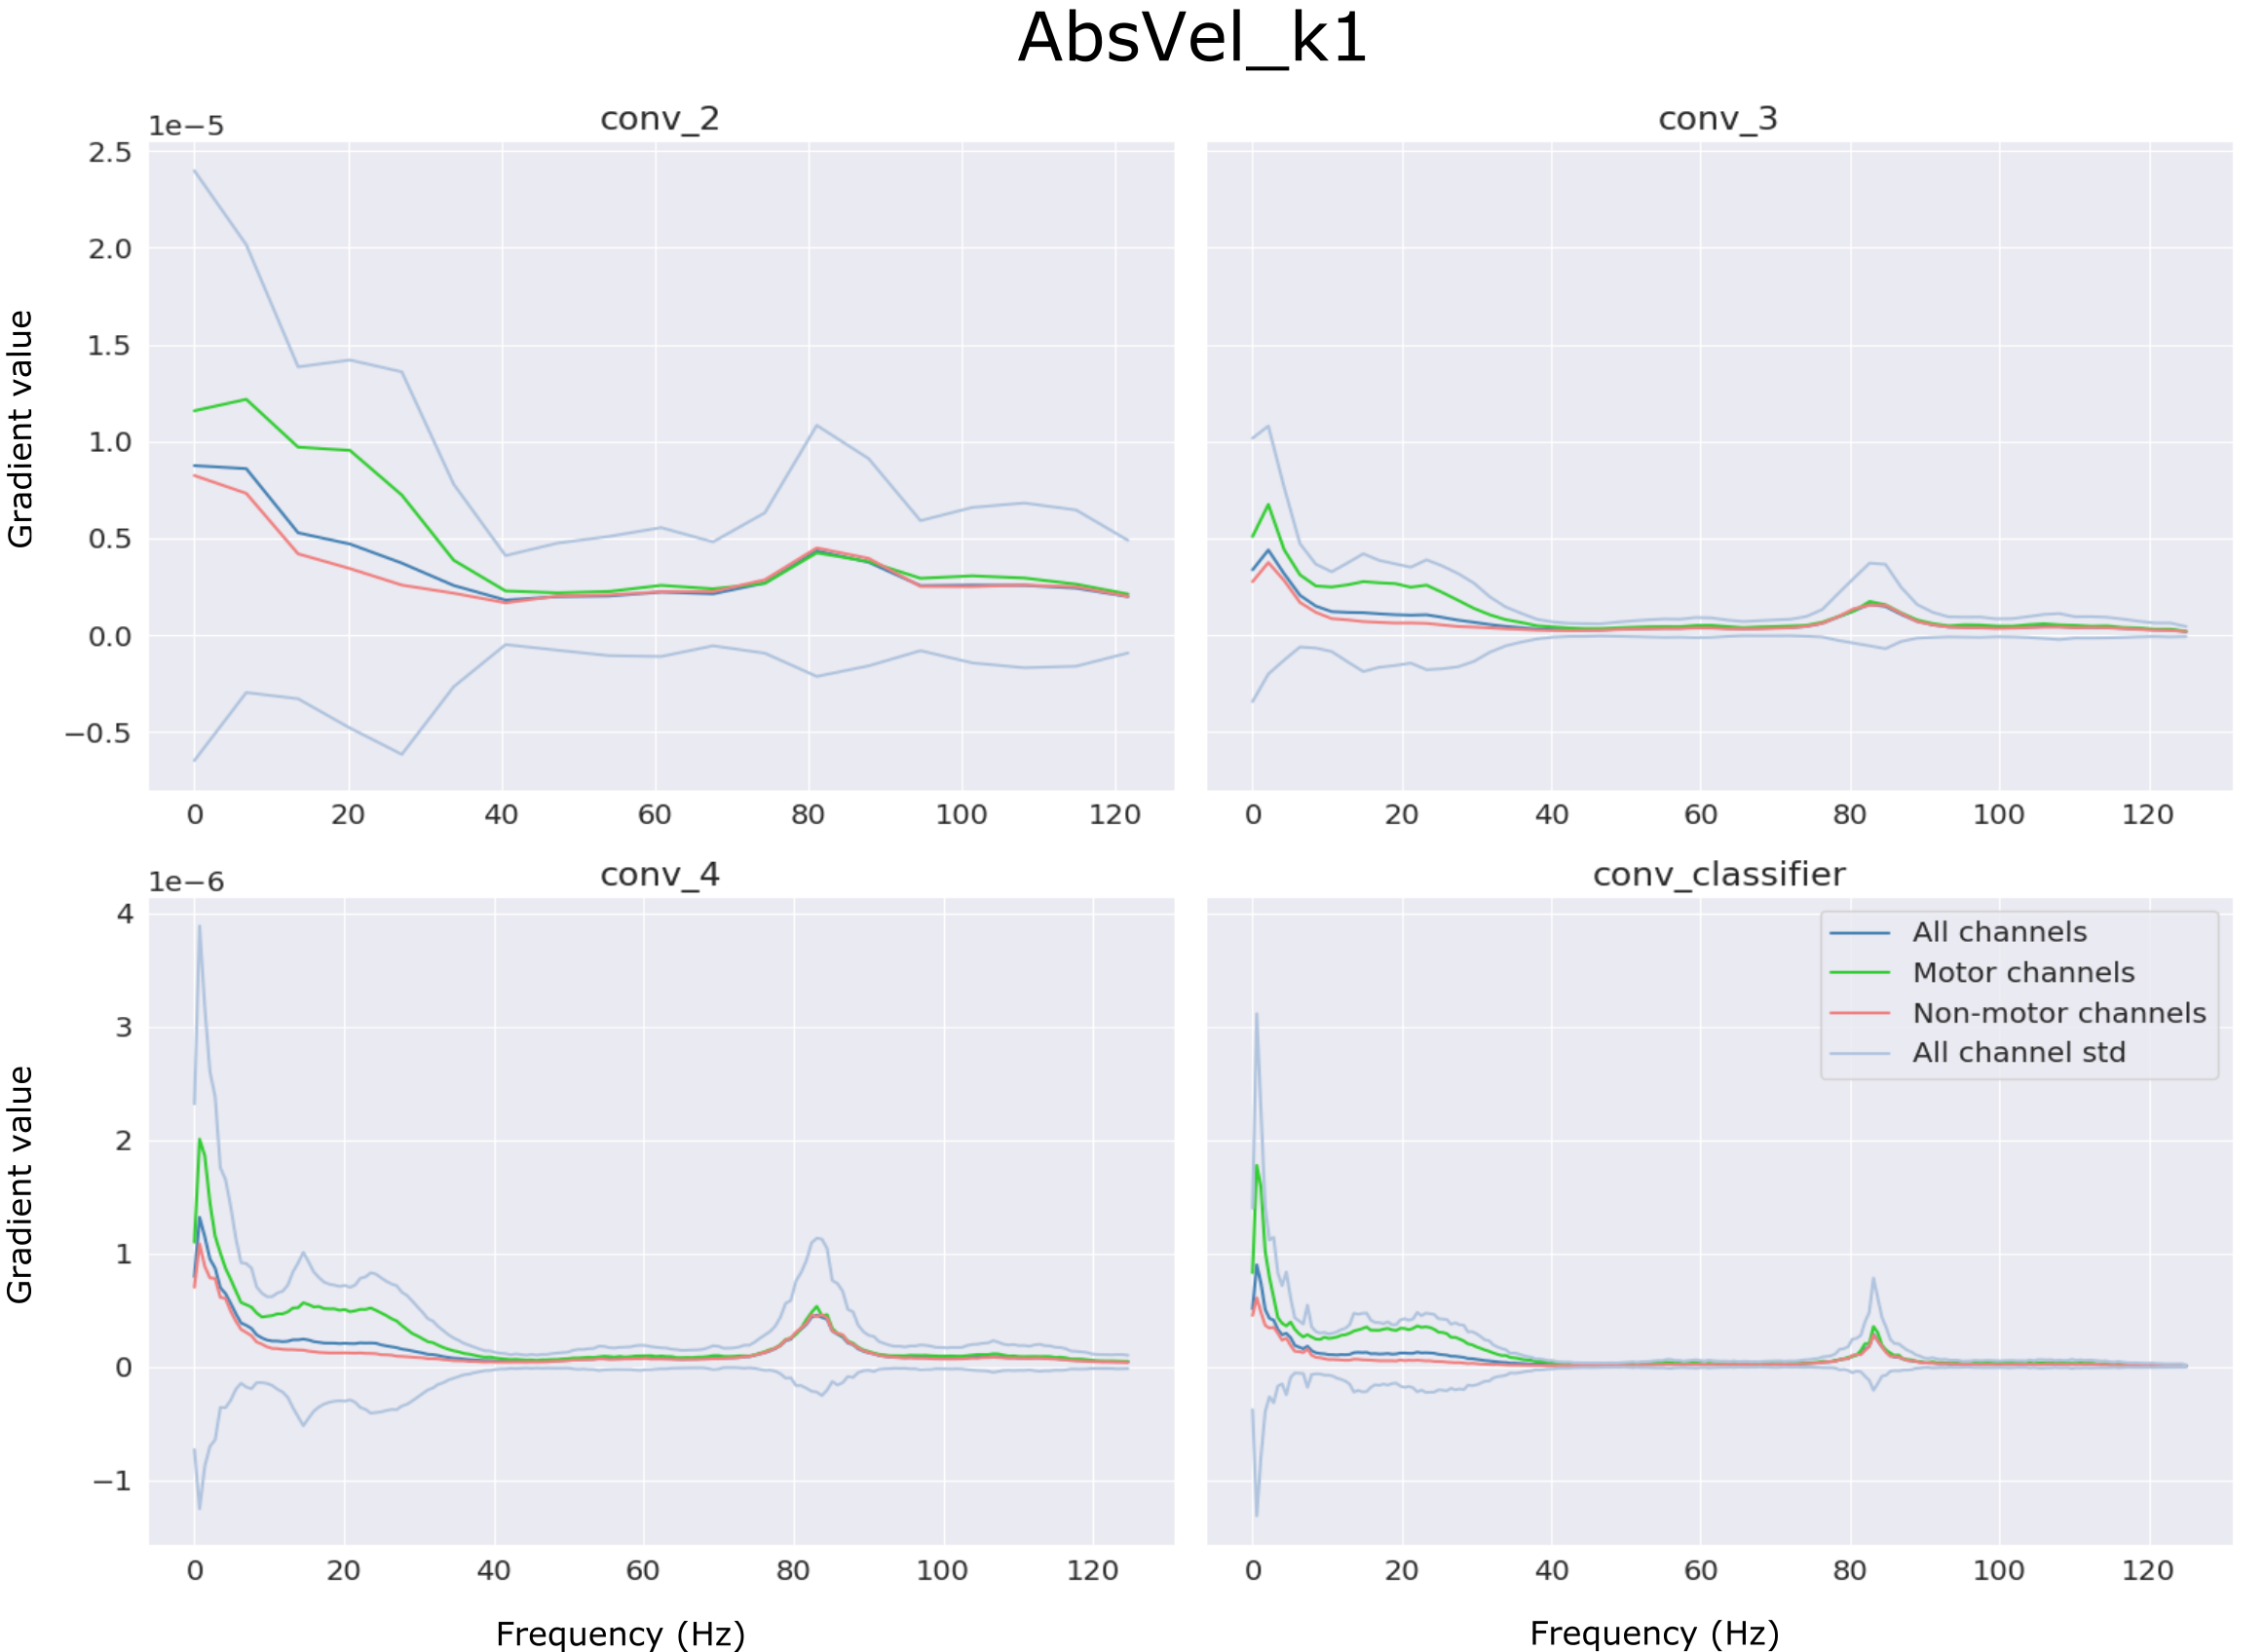
\includegraphics[width=.8\linewidth]{img/ch4/absVel-k1}
  \caption{1b}
  \label{fig:absVel-k1}
\end{subfigure}
\caption{plots of....}
\label{fig:gradient-peak}
\end{figure}

We also studied how the signal is affected by max-pool layers only.
We used one and three max-pool layers with dilations equivalent with those from the Deep4Net.
When the max-pool layer dilation parameter was three (or powers of three in the case of multiple consecutive max-pool layers), the output signal exhibited periodical peaks with the greatest peak around 83.33Hz.
When the dilation of the max-pool layers shifted to two and powers of two, the periodicity of the peaks still occurred, however, the period increased and the greatest peak was around 120Hz.
This is in line with the hypothesis that the alignment of frequencies with the max-pool layer dilations is indeed the reason for the gradient peak we see in Figure~\ref{fig:max-pool-changes}.

%\begin{figure}
%\begin{subfigure}{1\textwidth}
%  \centering
%  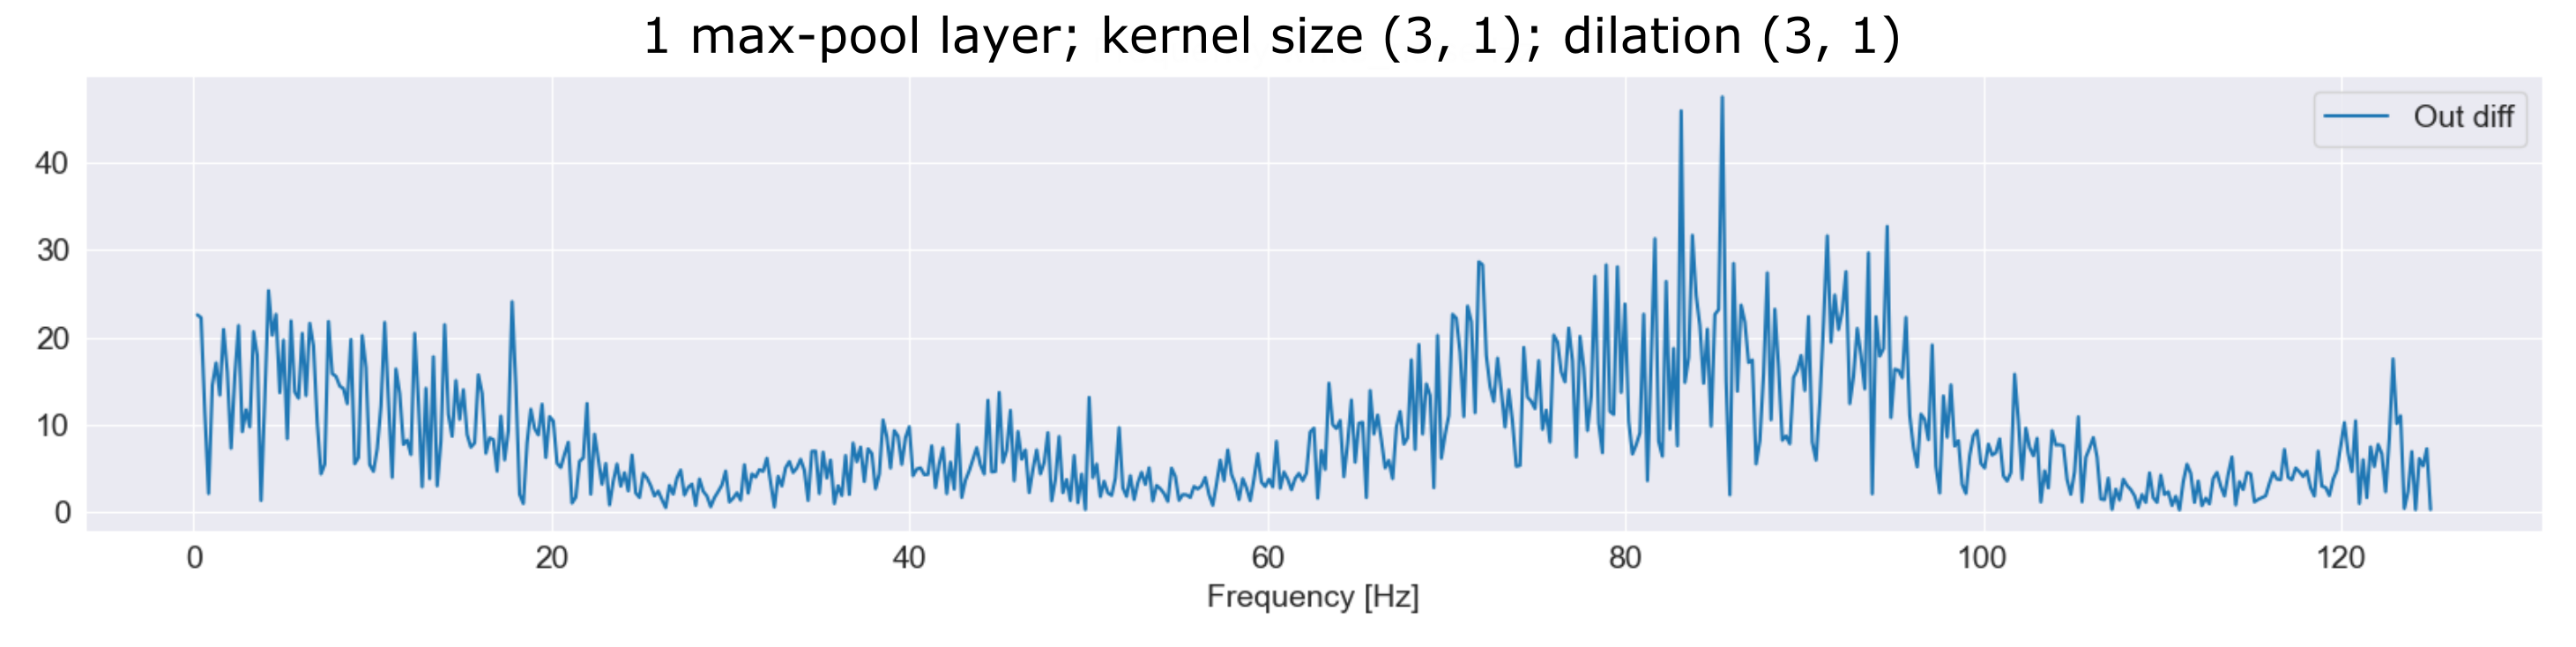
\includegraphics[width=1\linewidth]{img/ch4/absVel-maxpool-k3-d3}
%%  \caption{1a}
%  \label{fig:maxpool-k3-d3}
%\end{subfigure}%
%\begin{subfigure}{1\textwidth}
%  \centering
%  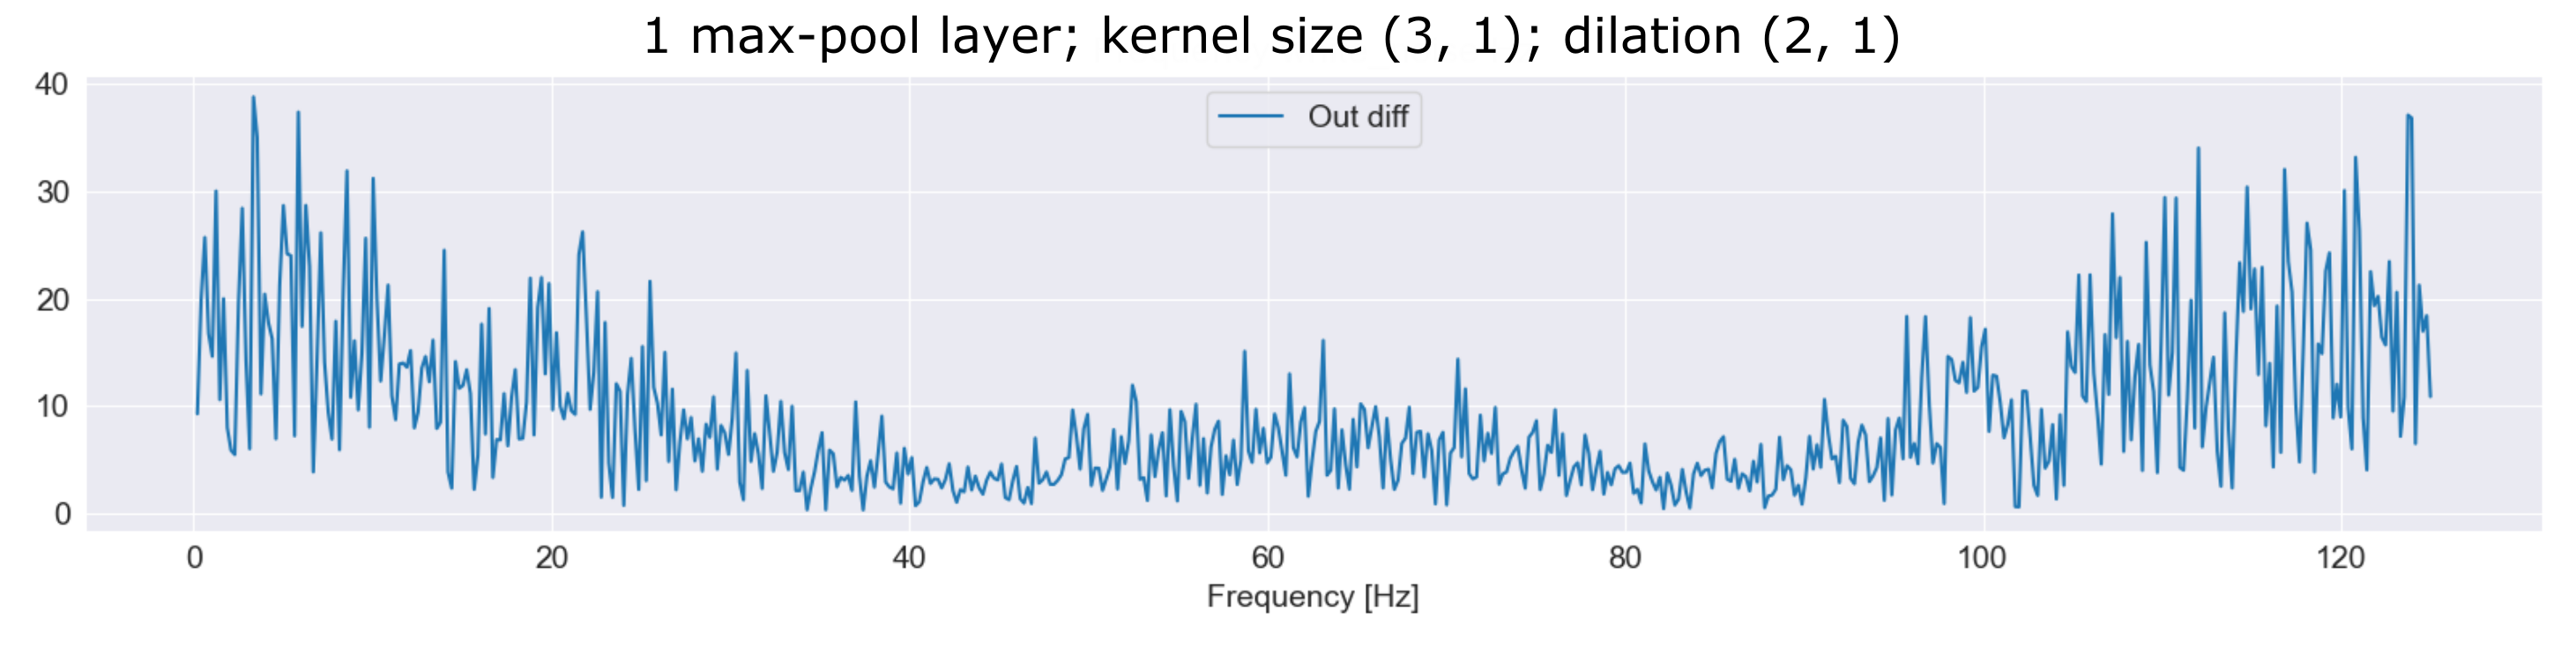
\includegraphics[width=1\linewidth]{img/ch4/absVel-maxpool-k3-d2}
%  \caption{1b}
%  \label{fig:maxpool-k3-d2}
%\end{subfigure}
%\caption{plots of....}
%\label{fig:max-pool-changes}
%\end{figure}%%

\begin{figure}
\centering
\begin{subfigure}[b]{\textwidth}
   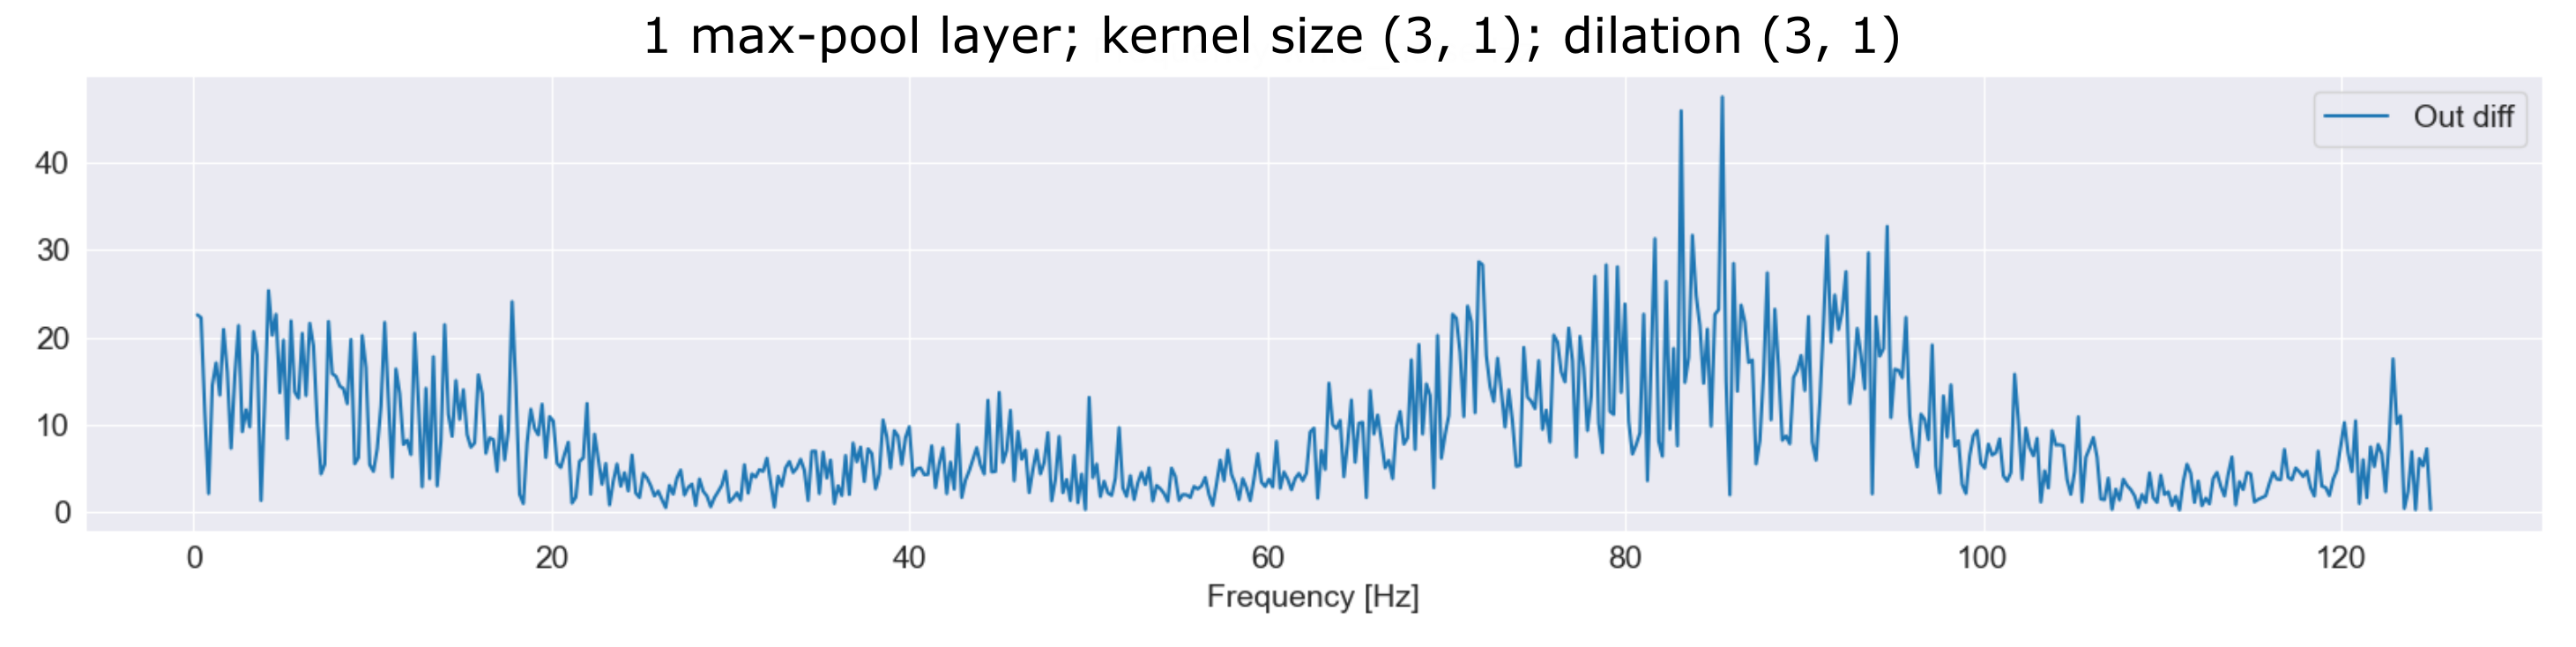
\includegraphics[width=1\linewidth]{img/ch4/absVel-maxpool-k3-d3}
   \caption{}
   \label{fig:Ng1} 
\end{subfigure}

\begin{subfigure}[b]{\textwidth}
   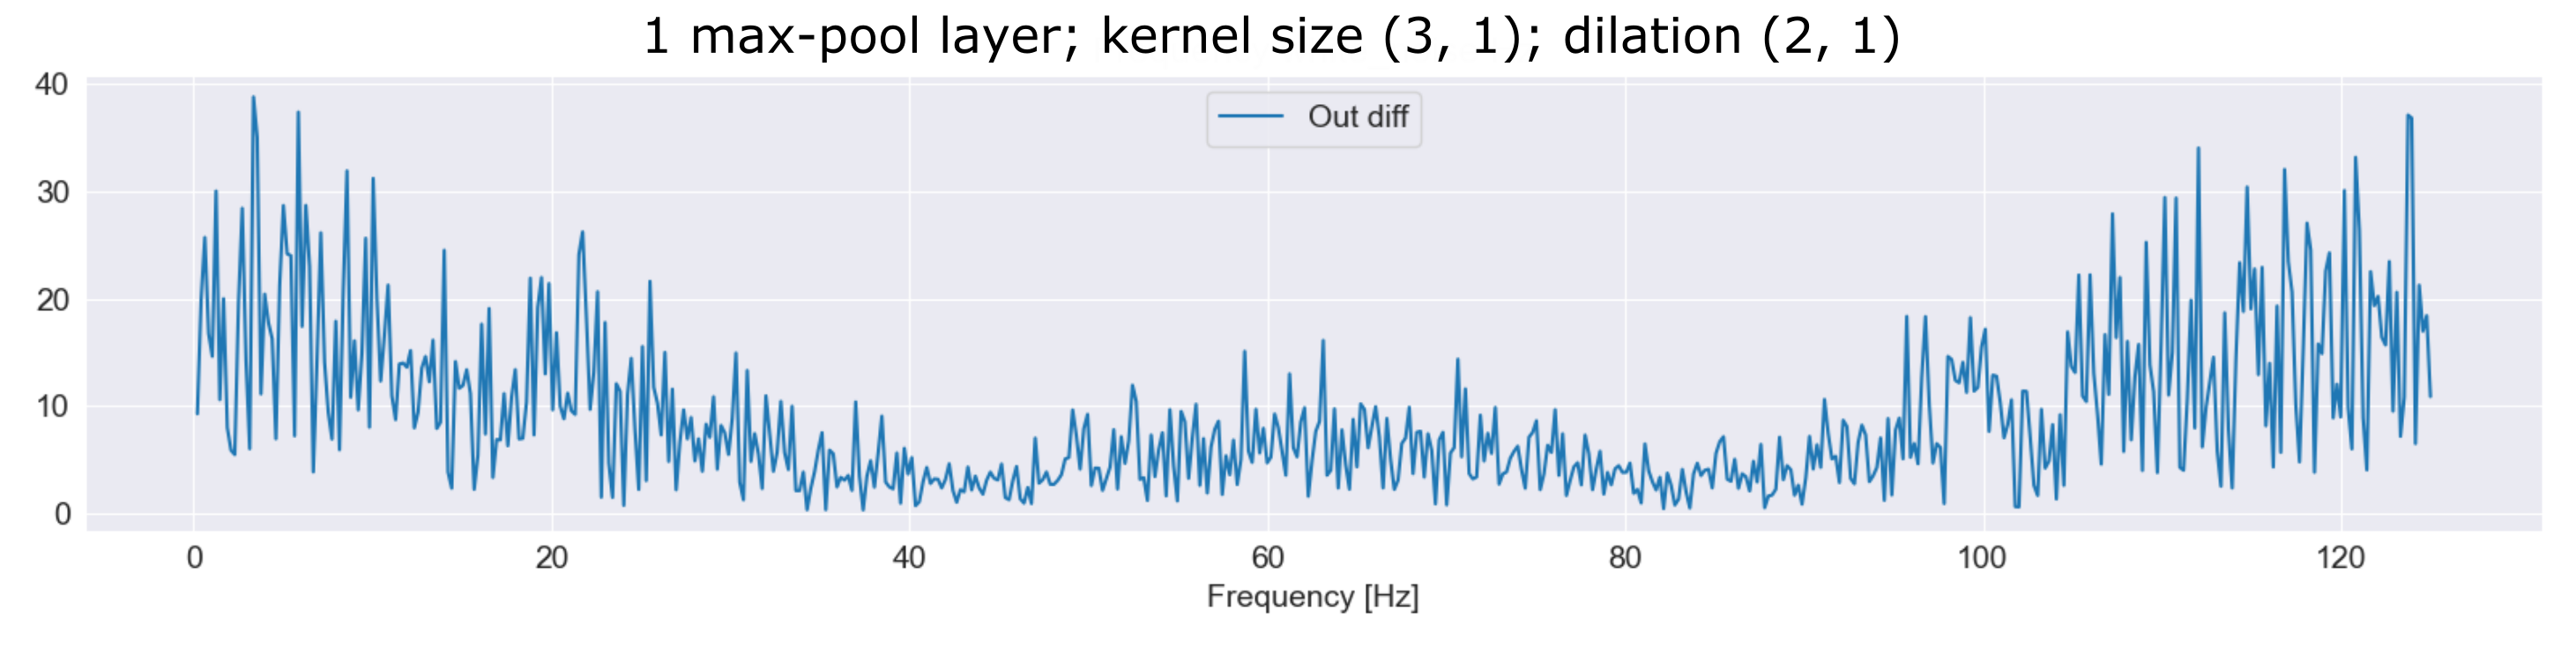
\includegraphics[width=1\linewidth]{img/ch4/absVel-maxpool-k3-d2}
   \caption{}
   \label{fig:Ng2}
\end{subfigure}

\caption[]{}
\end{figure}\label{fig:max-pool-changes}

The conclusions that can be made about the gradients peak when changing the kernel sizes and dilations of the max-pool layers are summarized below.
The majority of the above presented results suggests that the gradient peak is indeed the architecture artifact.
Its disappearance without loss of performance and the behaviour of the output signal when passed through single layers are in line with the hypothesis about frequency alignment.
The fact that the different kinds of channels (motor, non-motor) have similar gradient values at the peak also suggests that it only emerges because of the alignment.
If the motor channel gradients for the peak were visibly larger, it would support the hypothesis that some useful information is in this peak.
But because they are almost equal we can deduce that it is likely caused by the frequency alignment which should affect all channels in the same way.
The only argument speaking in favor of the gradient peak being informative for the network when making its decision is its amplification with training.
Nevertheless, this can be also attributed to the network not amplifying the peak but not actively working to suppress it as it occurs naturally when the signal passes through max-pool layers.
Lastly also the fact that the peak is also visible only when the input window is shortened to give only one output diminishes the credibility of the peak containing information useful for decoding.
Without the averaging, the gradient method is less stable and therefore also less reliable.
Overall, the gradient peak definitely cannot be taken as proof that the network is using high-gamma.

\section{Architectural modifications}\label{sec:architectural-modifications}
\subsection{Performance}\label{subsec:performance}
While the gradient peak seemed like a dead end, while studying it, we noticed that some of the networks, especially those with smaller kernel sizes and/or dilation parameters in their max-pool layers seem to perform significantly better.
Therefore, we decided to do a thorough inspection of how each of the networks performs on the filtered datasets as described in Section~\ref{subsec:modifications-to-the-dataset}.
The results can be seen in Figure~\ref{fig:original-performances-velocity} for velocity and Figure~\ref{fig:original-performances-absolute-velocity} for absolute velocity.
In the following points we summarize the findings on the different datasets.

\begin{itemize}
    \item \textbf{Full training and validation} Some of the networks significantly outperformed the Deep4Net sbp0 when both trained and validated on full data. The best performing network was the network where the max-pool layer had no influence, namely the one with max-pool layer kernel size 1.
    \item \textbf{Full training and low-pass validation} When the networks were trained on the full dataset and validated on the low-passed dataset (< 40Hz), the performance changed significantly for all the networks as is obvious from the Figure~\ref{fig:original-performances}.
    Nevertheless, in order to achieve a statistically significant decrease in performance, we had to use a Butterworth filter of order 15 instead of order 3 which was previously used inZ\cite{Hammer-2021}.The 3rd order filter caused no apparent change in performances.
    The Butterworth filter gradually attenuates the frequencies above the cut-off frequency (40Hz in this case).
    The higher the filter order, the steeper the attenuation is.
    Therefore, the fact that the performance decrease followed only after the stronger filter was employed suggests, that the network indeed focuses on frequencies above 40Hz but not particularly high frequencies (those in the high-gamma band) which were attenuated by both the 3rd as well as 15th order filter Figure~\ref{fig:filters}.
    \item \textbf{High-pass training and validation} To see if the networks are able to use information from the high-gamma frequency band at all, the networks were trained and evaluated on the high-pass dataset (>60Hz).
    As is clear from Figure~\ref{fig:original-performances}, the networks are able to use some information from the high-gamma especially when decoding absolute velocity where the correlations are often not only significantly above chance decoding but also achieve fairly good correlation coefficients.
    \item \textbf{Full training and high-pass validation} A possibility to find out if the networks when trained on full data are learning from the high-gamma frequency band, is to train the network on the full dataset and validate only on the high-passed data.
    Therefore we also explored this option.
    It is obvious from Figure~\ref{fig:original-performances} that only few networks perform significantly better than chance level decoding.
    The conclusion that the network, when given access to, utilizes primarily information from the low end of the frequency spectrum can be drawn from this result.
    \item \textbf{Low-pass training and high-pass validation}
    Training on low-passed data and validation on high-passed data was also important to further study how the network operates.
    We wanted to find out if it is able to somehow transfer information between two completely separate datasets.
    Because the cut-off frequency for the low-passed data is 40Hz and for the high-passed data 60Hz with a very steep filter, there is no frequency overlap between the two sets.
    Therefore, it would be interesting but also rather surprising if from modulation in the low frequencies (below 40Hz) the network would learn to use information about modulations in the high frequencies (above 60Hz).
    Nevertheless, as obvious from Figure~\ref{fig:original-performances}, the networks were unable to transfer any information.
    
\begin{figure}[!htpb]
\centering
\begin{subfigure}[b]{\textwidth}
   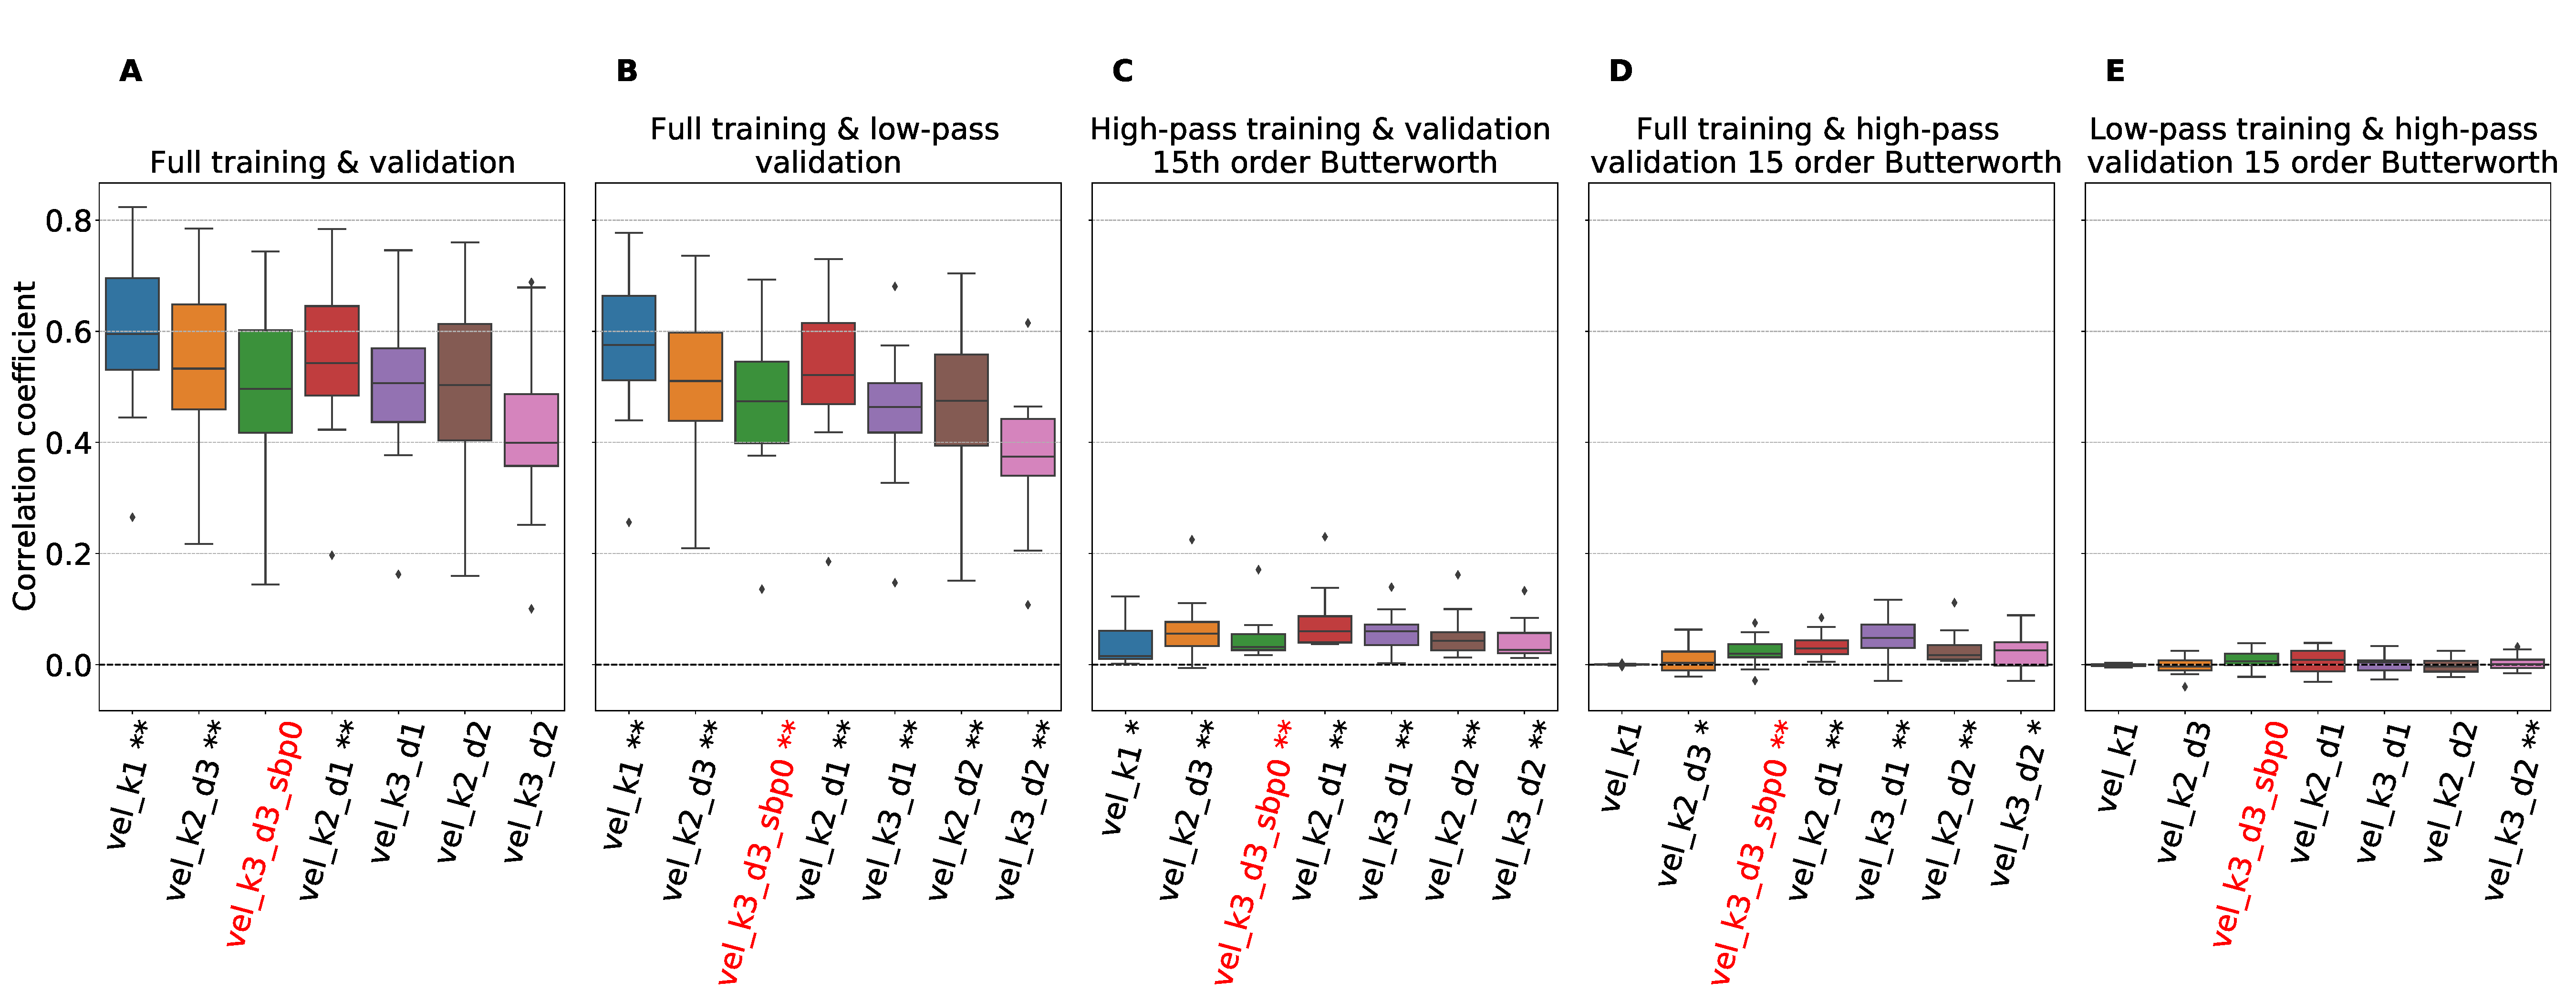
\includegraphics[width=1\linewidth]{img/ch4/original_setting_vel_performance_comparison}
   \caption{}
   \label{fig:original-performances-velocity} 
\end{subfigure}

\begin{subfigure}[b]{\textwidth}
   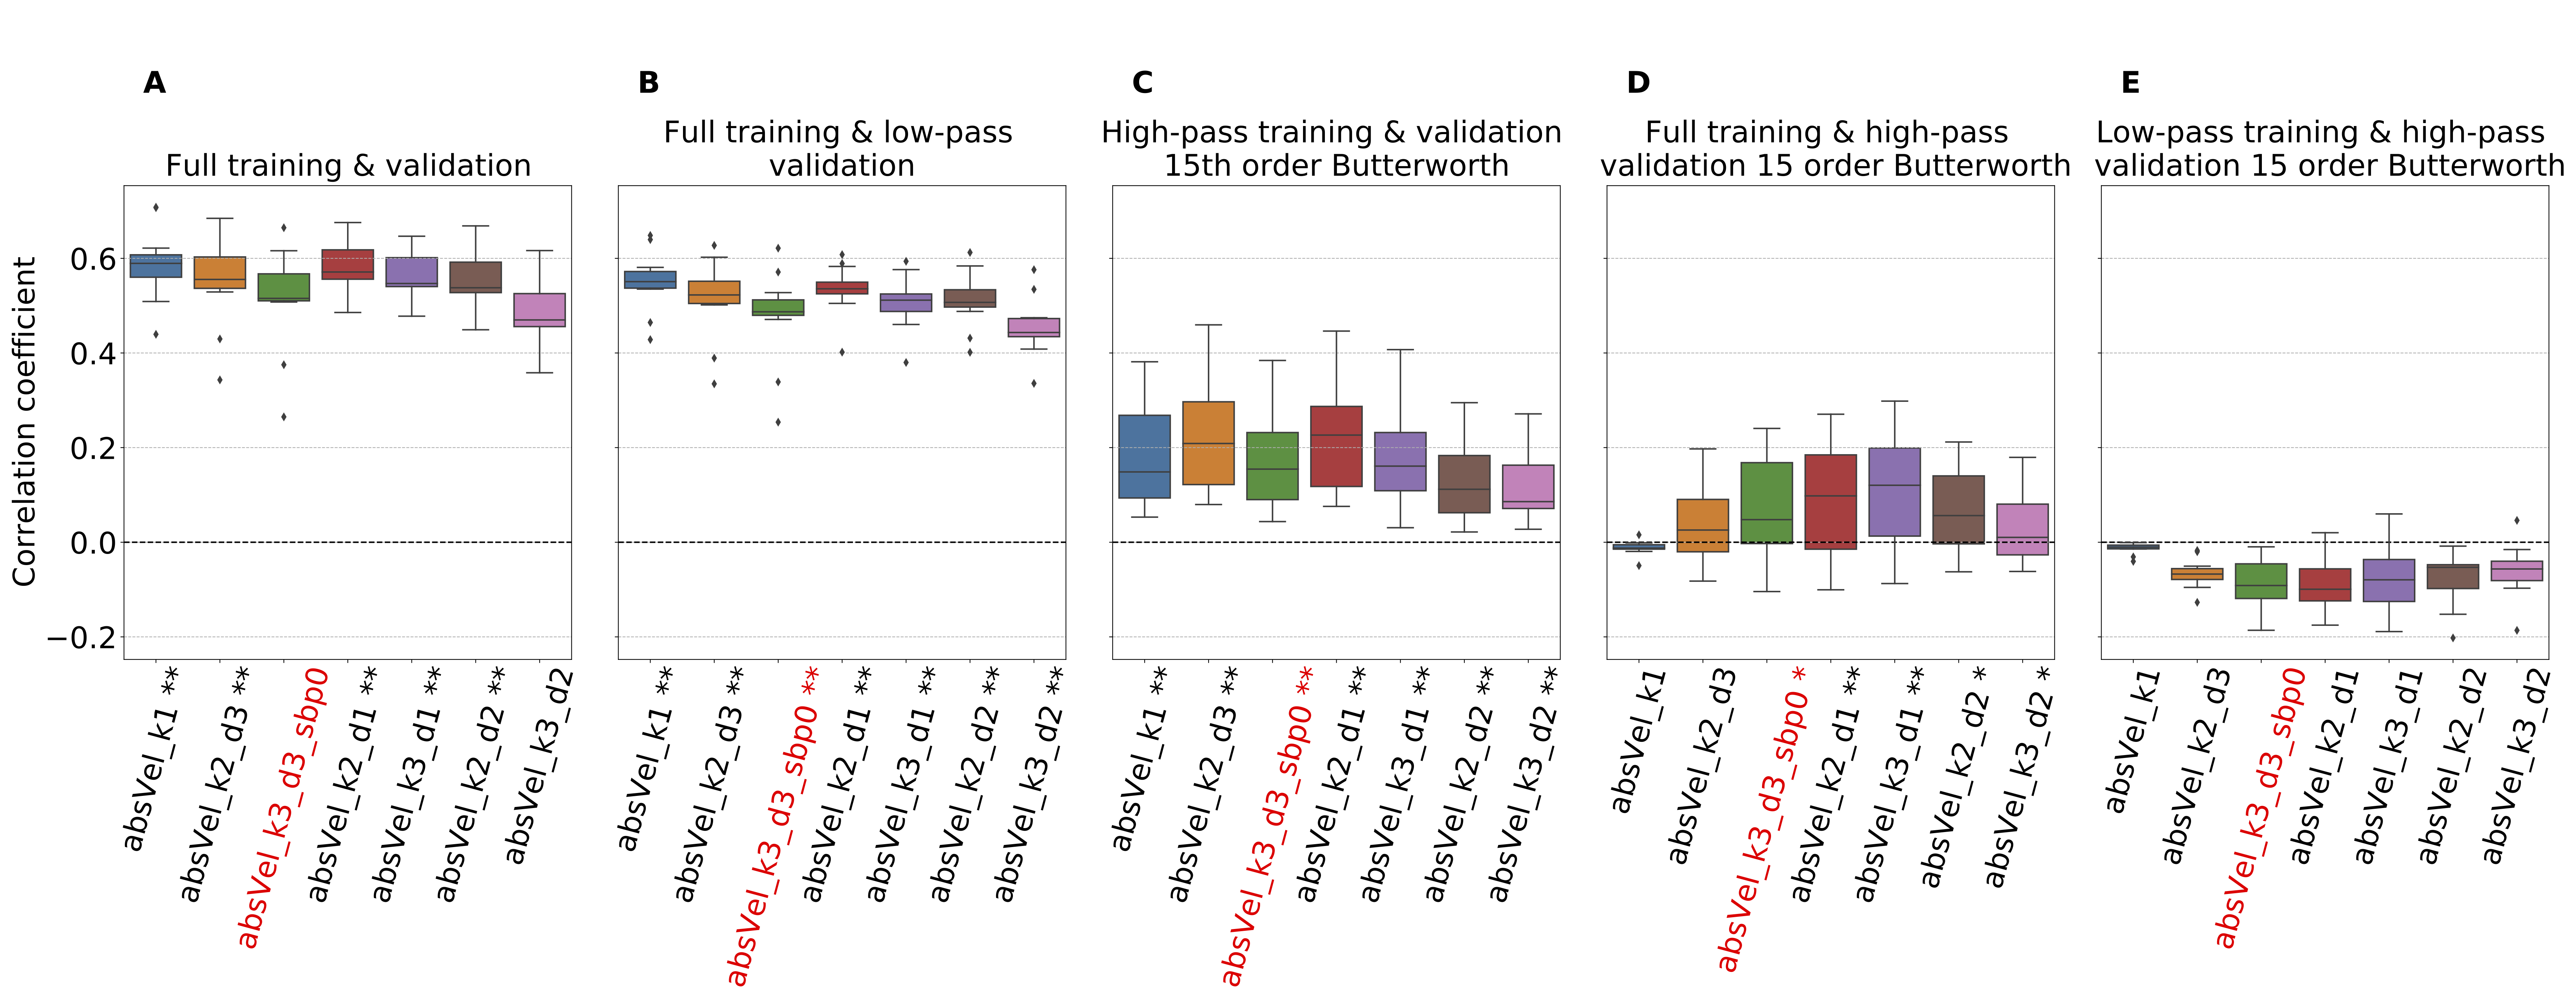
\includegraphics[width=1\linewidth]{img/ch4/original_setting_absVel_performance_comparison}
   \caption{}
   \label{fig:original-performances-absolute-velocity}
\end{subfigure}
\caption[]{}
\end{figure}\label{fig:original-performances}


\end{itemize}

The findings presented in this section lead to two interesting questions.
The first one  is what do the gradients of the various architectures look like and do some of them use high-gamma?
This analysis is described in Section~\ref{subsec:gradients}.
The second question that arises if we notice, that the performance seems to drop with increasing size of the receptive field \cref{fig:distance-from-rf}.
Networks with a smaller receptive field seem to perform better possibly because the predicted time-point is closer to the centre of the receptive field.
Therefore, it is interesting to see what happens when we shift the predicted time-point to the centre of the receptive field.
More details and the analysis are described in Section~\ref{sec:shifting-the-predicted-time-point}.

\begin{figure}[!htpb]
\centering
\begin{subfigure}[b]{0.65\textwidth}
   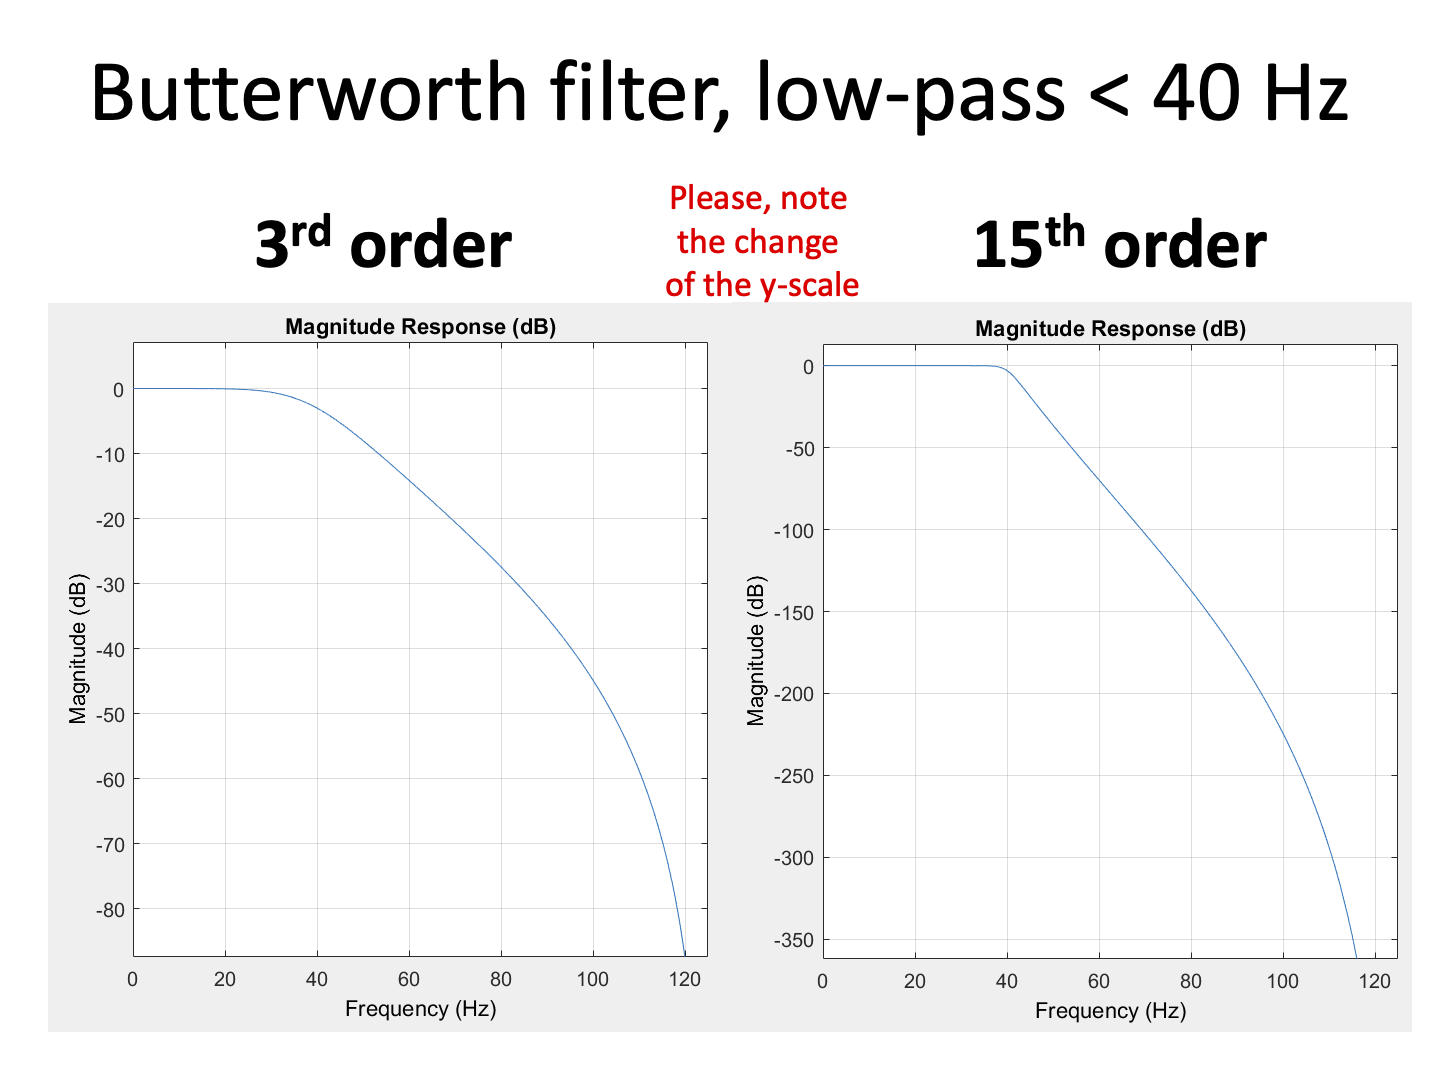
\includegraphics[width=1\linewidth]{img/ch3/lp-butterworth-filter}
   \caption{}\label{fig:lp-filters}
\end{subfigure}

\begin{subfigure}[b]{0.65\textwidth}
   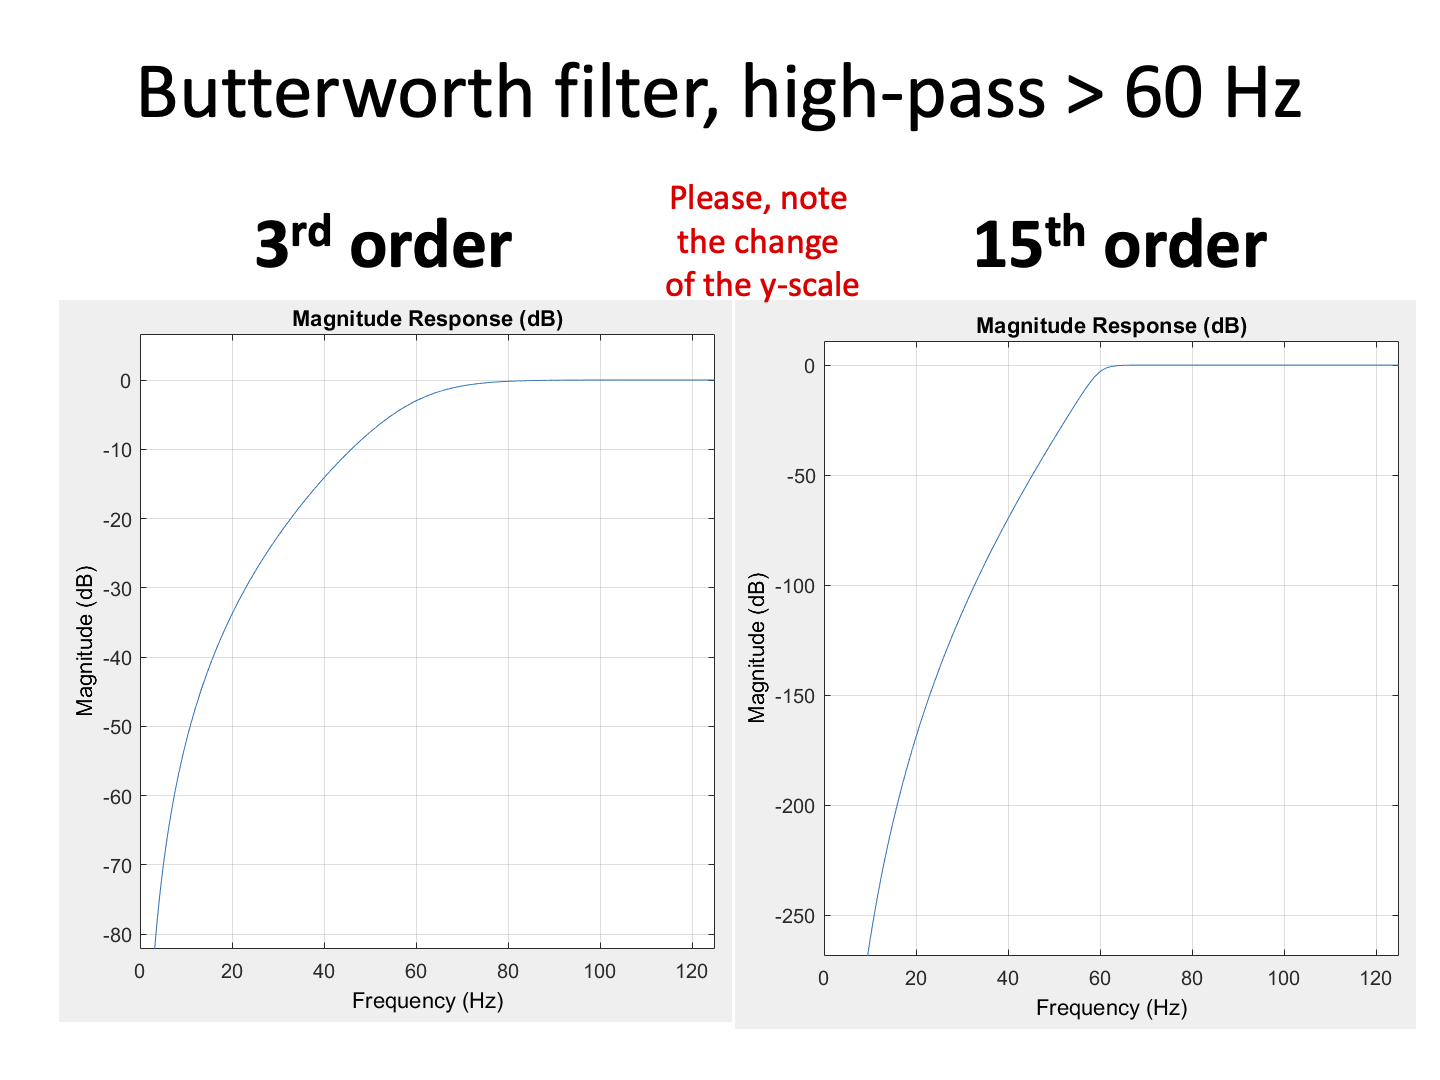
\includegraphics[width=1\linewidth]{img/ch3/hp-butterworth-filter}
   \caption{}
\end{subfigure}
\caption[]{}\label{fig:hp-filters}
\end{figure}\label{fig:filters}

\subsection{Gradients}\label{subsec:gradients}
The differences in performance among the networks, reinforce the interest in the gradients of the various architectures.
Since some of the networks perform significantly better compared to the initial Deep4Net, we analyze gradients of the different architectures to see if the reason for a better performance is their ability to use information from the high-gamma band.
We perform the gradient visualization of all the architectures with kernel sizes 1, 2 and 3 and dilations as powers of 1, 2 and 3.

The results show differences in gradients among the architectures.
Gradients of all intermediate layers and the visualizations can be found in the Appendix.
Figure~\ref{fig:last-layer-grads} includes the gradients of the output layer which in our opinion best represents the gradients of the other layers for all the architectures.

\begin{figure}[!htpb]
\centering
\begin{subfigure}[b]{\textwidth}
   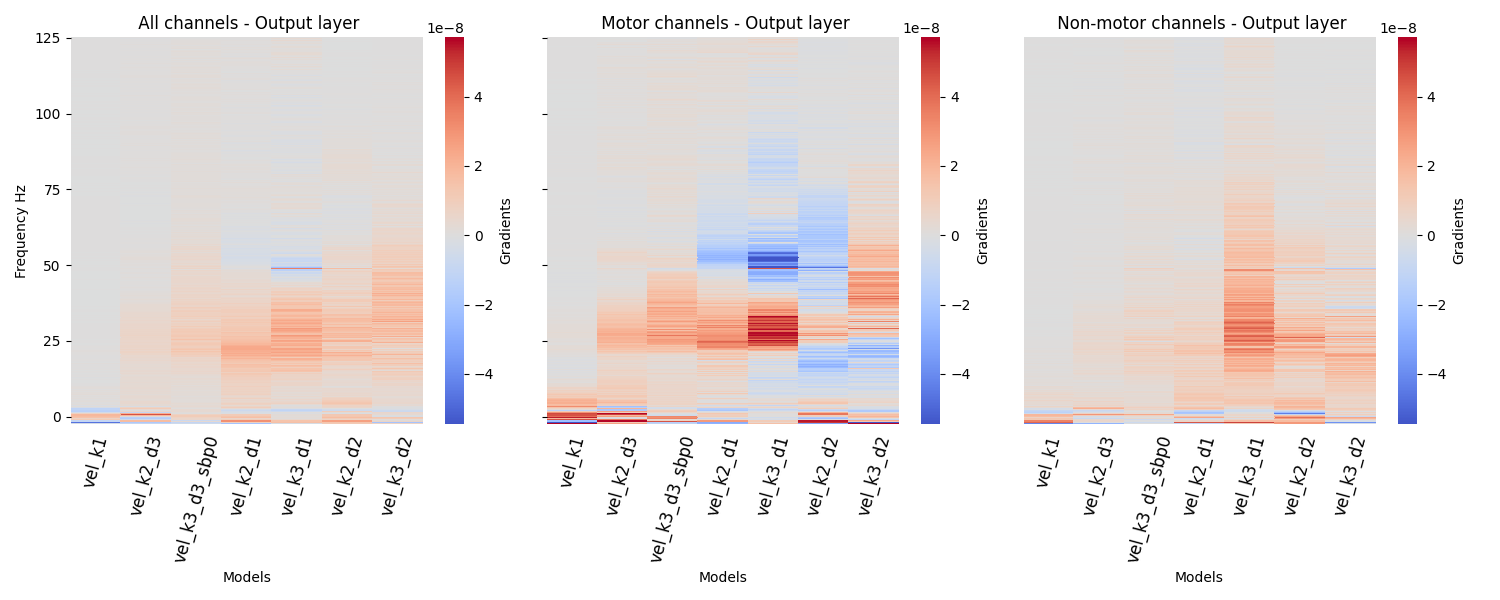
\includegraphics[width=1\linewidth]{img/ch4/vel-last-layer-grads}
   \caption{}
\end{subfigure}\label{fig:absVel-last-layer-grads}

\begin{subfigure}[b]{\textwidth}
   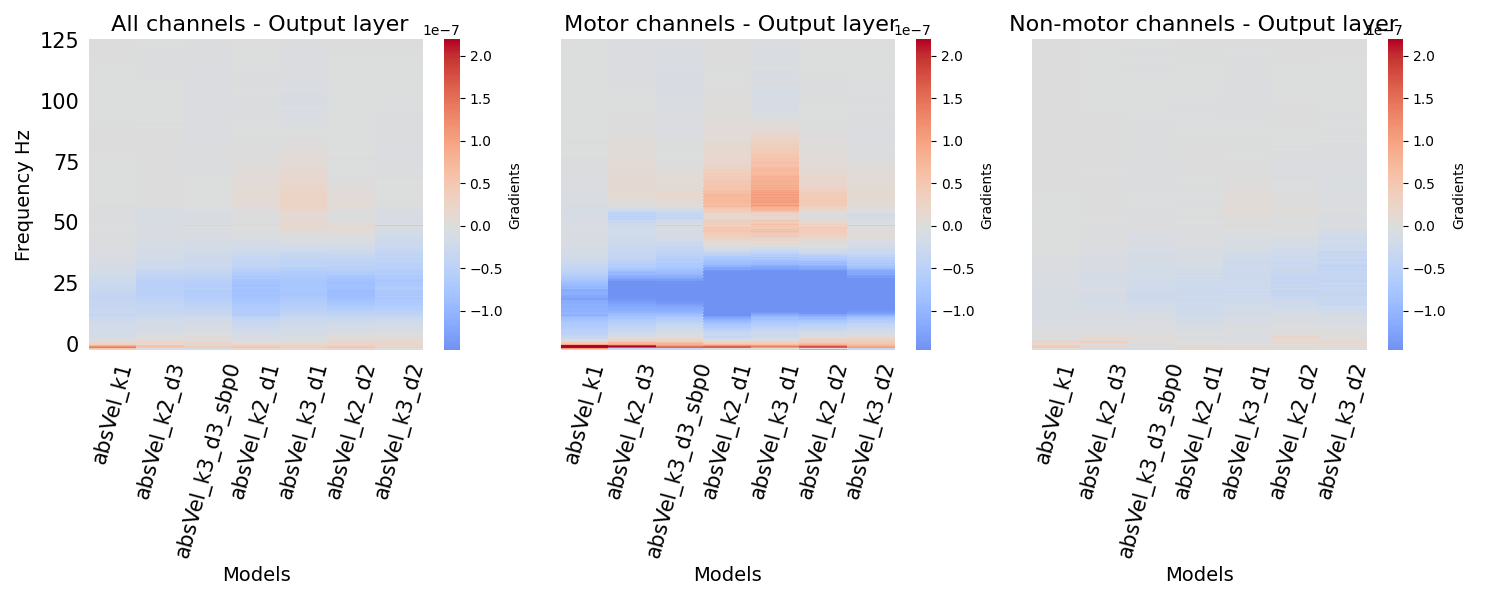
\includegraphics[width=1\linewidth]{img/ch4/absVel-last-layer-grads}
   \caption{}
\end{subfigure}\label{fig:vel-last-layer-grads}
\caption[]{}
\end{figure}\label{fig:last-layer-grads}

Based on the performances of the networks presented in Section~\ref{subsec:performance} and the gradients presented in this Section these important and interesting observations can be made:

\begin{itemize}
    \item The networks focus on motor-channels when making predictions.
This is to be expected when they are tasked with decoding movement.
    \item There are obvious differences between the gradients for velocity and absolute velocity.
    Nevertheless, for both variables the network without max-pool, here denoted as {variable}\_k1 is the best performing architecture.
    And it is in both cases also the network which is most interested in modulations in the low frequency bands.
    This suggests that using the information in the high-gamma frequency band is not necessarily an asset.
    \item The networks which exhibit higher interest in information from the higher frequencies, namely the k2\_d1, k3\_d1 and k2\_d2 are also those, which are able to perform significantly above chance when trained on full data and validated on high-passed data.
    This suggests consistency between the gradient visualization and the performance analysis.

\end{itemize}


\section{Shifting the predicted time-point}\label{sec:shifting-the-predicted-time-point}
In this section we describe how the performance and gradients change when the predicted time-point is shifted with respect to the receptive field.
Two kinds of analyses are introduced here.

\begin{enumerate}
    \item Shifting the predicted time-point to the centre of the receptive field
This analysis was performed on all the network architectures and compares how the different architectures react to the shift both performance-wise and gradient-wise.
We highlight the differences and similarities between the architectures.
    \item Shifting the predicted time-point in steps across the receptive field
This analysis was performed only on the original Deep4Net sbp0.
It compares how the performance and gradients of the network change when the predicted time-point is shifted across the receptive field using a different ratio of information from the future and from the past.
\end{enumerate}


\subsection{Shifting the predicted time-point to the centre of the receptive field}\label{subsec:shifting-the-predicted-time-point-to-the-centre-of-the-receptive-field}
An important observation when looking at the performance of the different architectures described in Section\ref{sec:architectural-modifications} was made.
We noticed that the smaller receptive field seemingly correlates with a higher prediction accuracy especially for absolute velocity decoding.
To visualize this, we created Figure~\ref{fig:figure-distance} which sorts the different architectures based on the size of the receptive field from smallest to largest and plots the average correlation coefficient each of these networks achieved.
There is a clear descending pattern especially for absolute velocity where the only exceptional network is the k2\_d3 network which performs well with a large receptive field.

\begin{figure}
\centering
   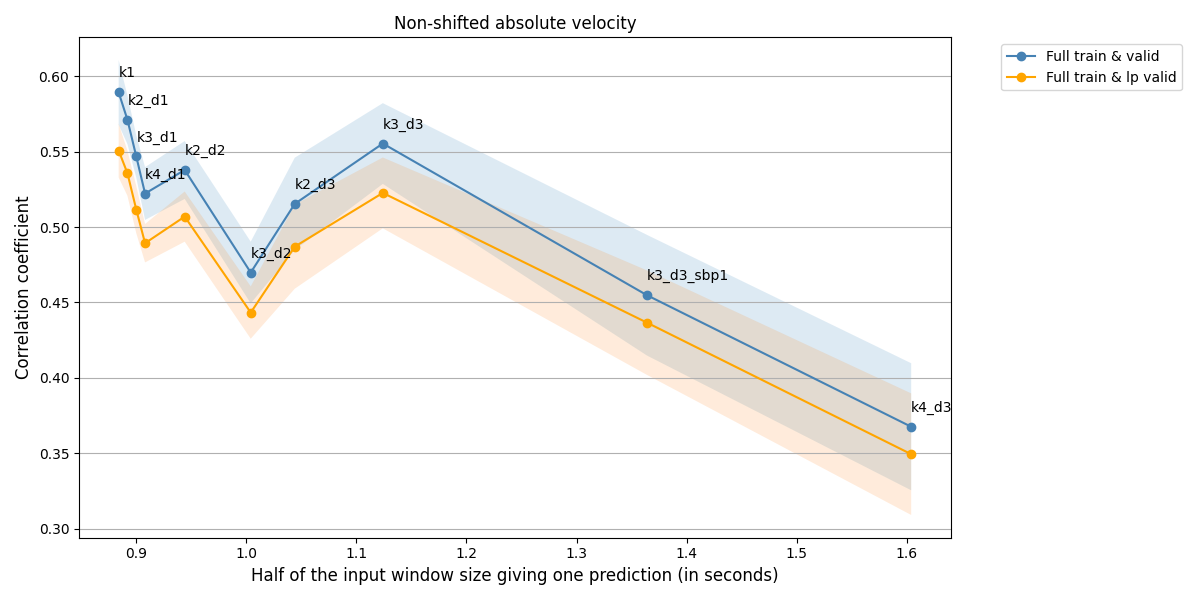
\includegraphics[width=1\linewidth]{img/ch4/distance-shifted-performance-absVel}
   \caption{}
\end{figure}\label{fig:figure-distance}

This finding further corroborates the idea to shift the predicted time point to the center of the receptive field.
The receptive field as described in Section~\ref{subsec:receptive-field} is non-uniform.
It considers mostly input-points in its centre while in the original decoding, the predicted time-point is located just outside the receptive field.
Therefore, we shift the inputs and prediction so that the iEEG signal, which was recorded at the same time as the predicted movement was executed, is in the centre of the receptive field and present how this affects the performance and gradients of the various architectures.
This causes the procedure to be unsuitable for online BCI because half of the input window uses information from the future.
\subsubsection{Performance}
The results can be seen in Figure~\ref{fig:shifted-performance}.
It is obvious that the shift greatly improves performance of all the networks and the performance differences between the architectures are diminished.
Notably the performance of the networks on the high-gamma dataset also increased especially for absolute velocity.
\begin{figure}[!htpb]
\centering
\begin{subfigure}[b]{\textwidth}
   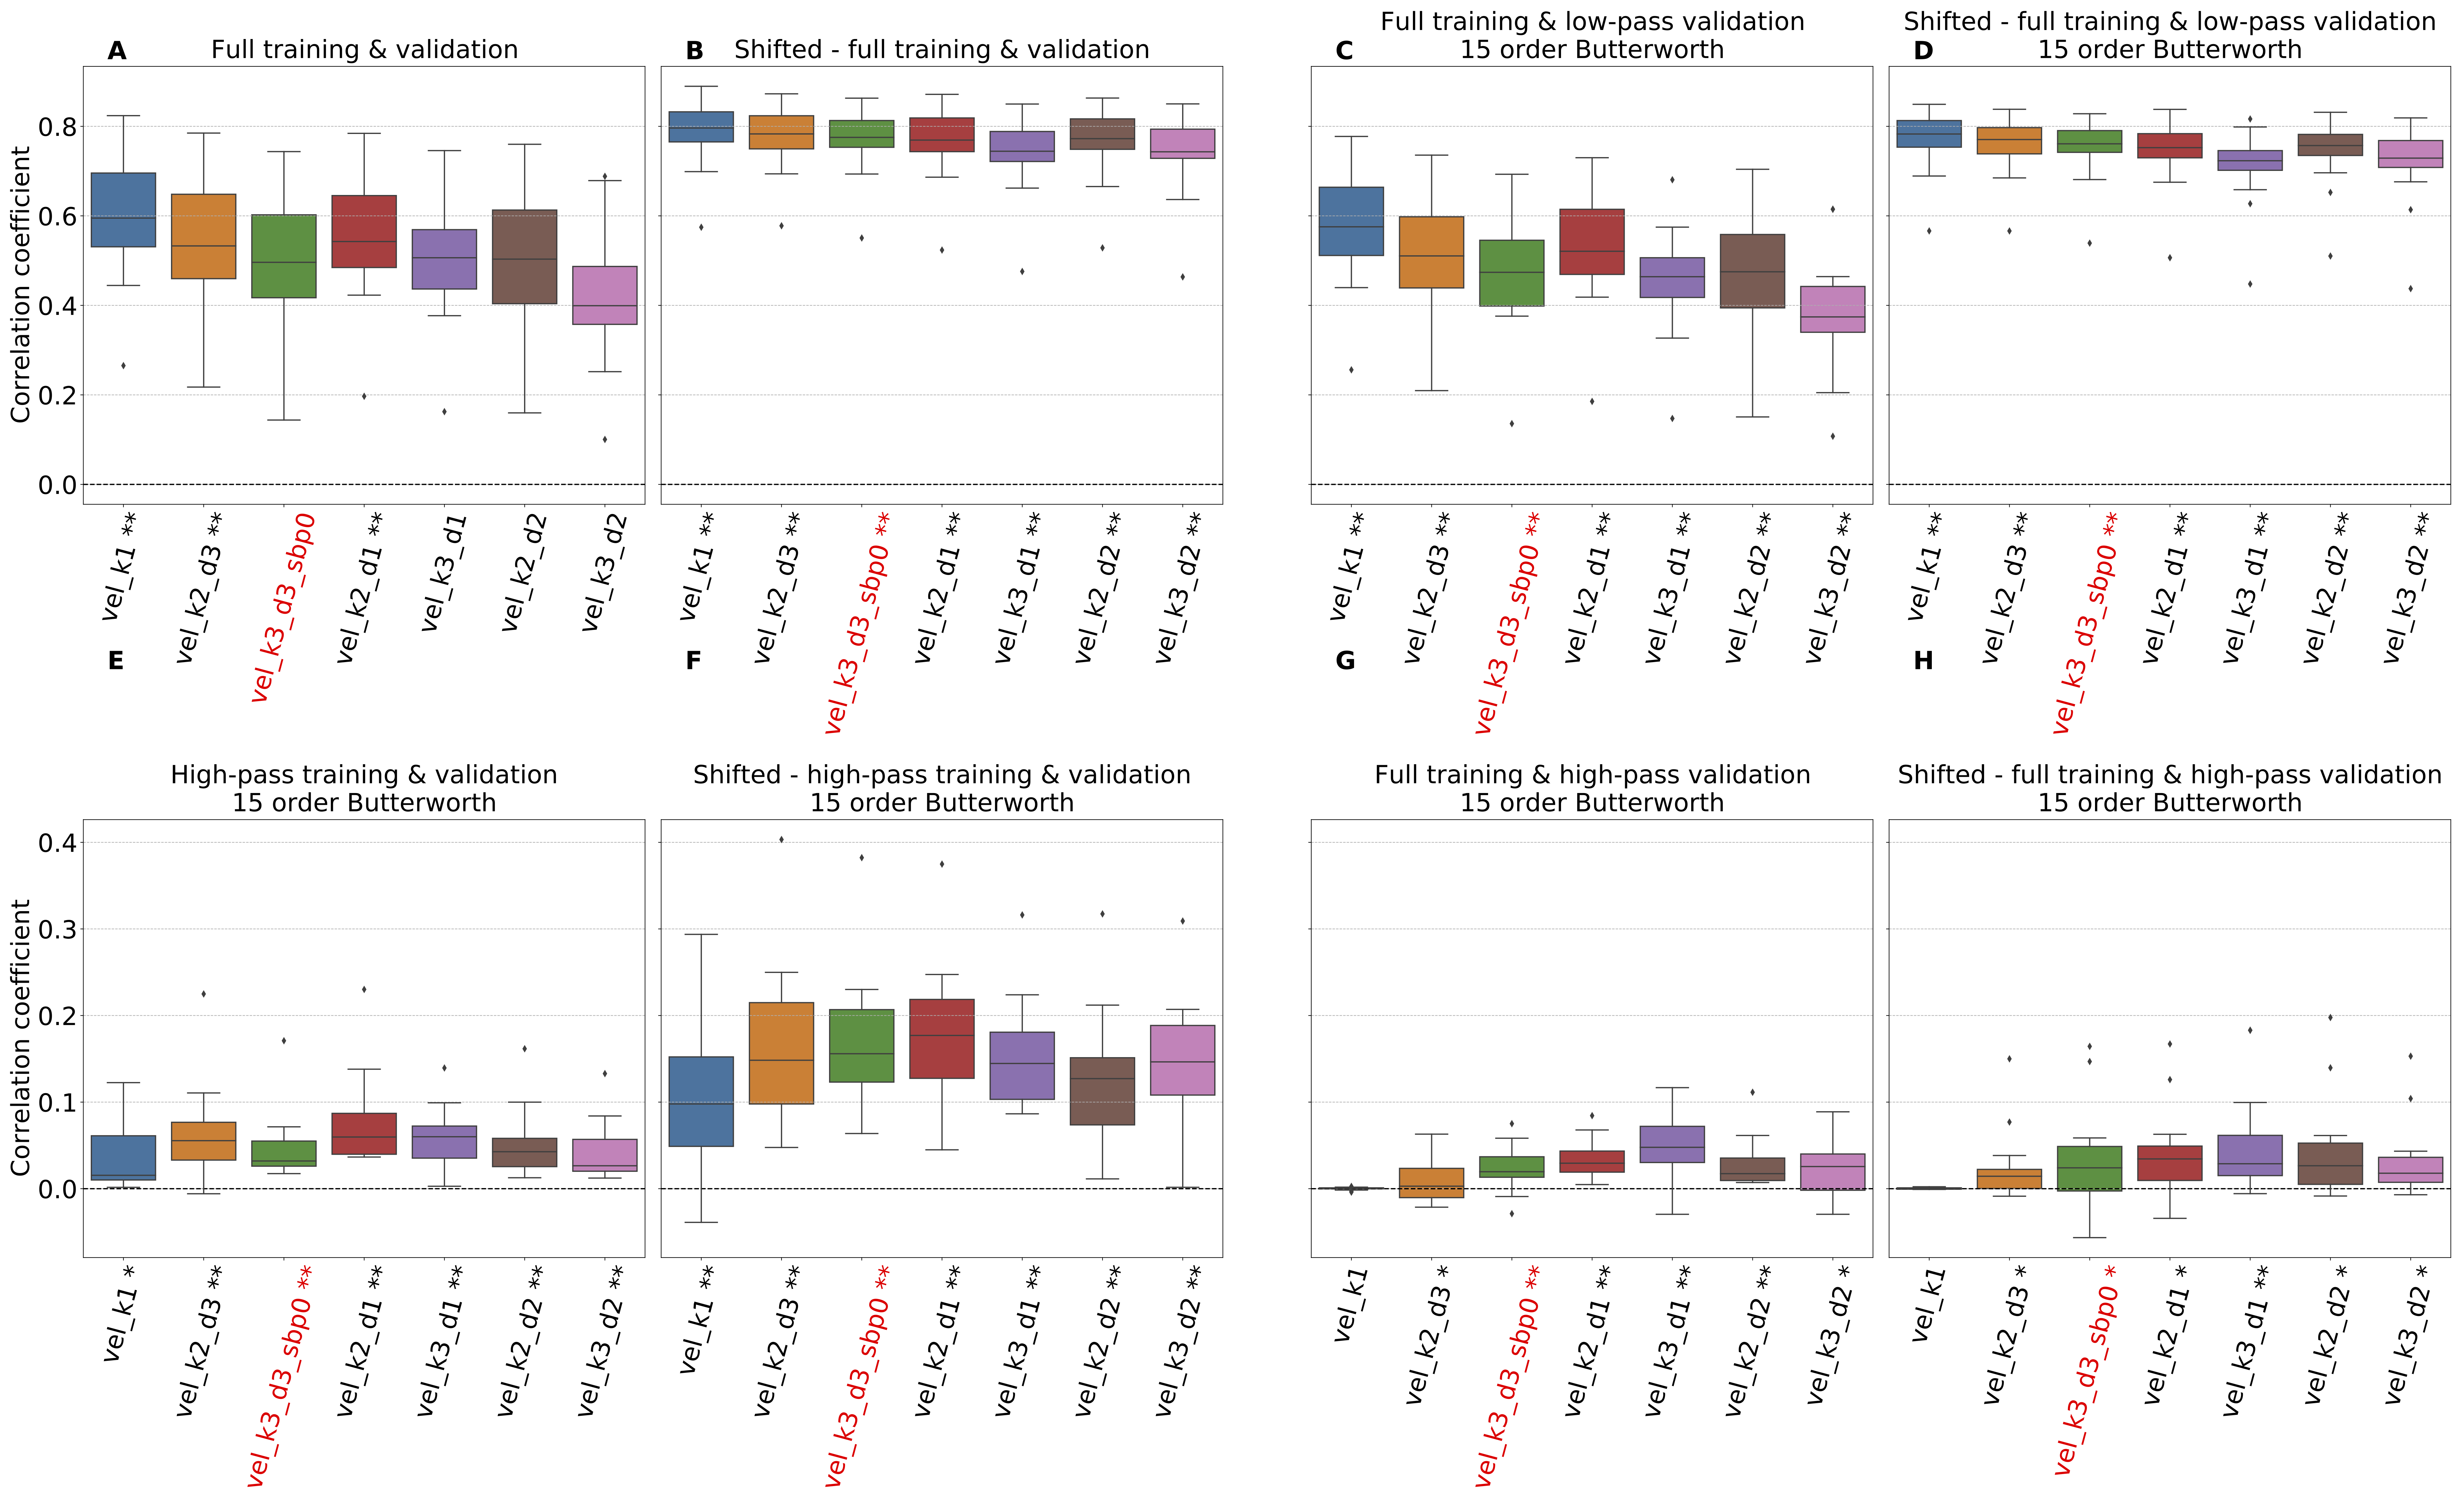
\includegraphics[width=1\linewidth]{img/ch4/shifted_vs_non_shifted_vel_performance_comparison}
   \caption{}
\end{subfigure}\label{fig:shifted-performance-vel}

\begin{subfigure}[b]{\textwidth}
   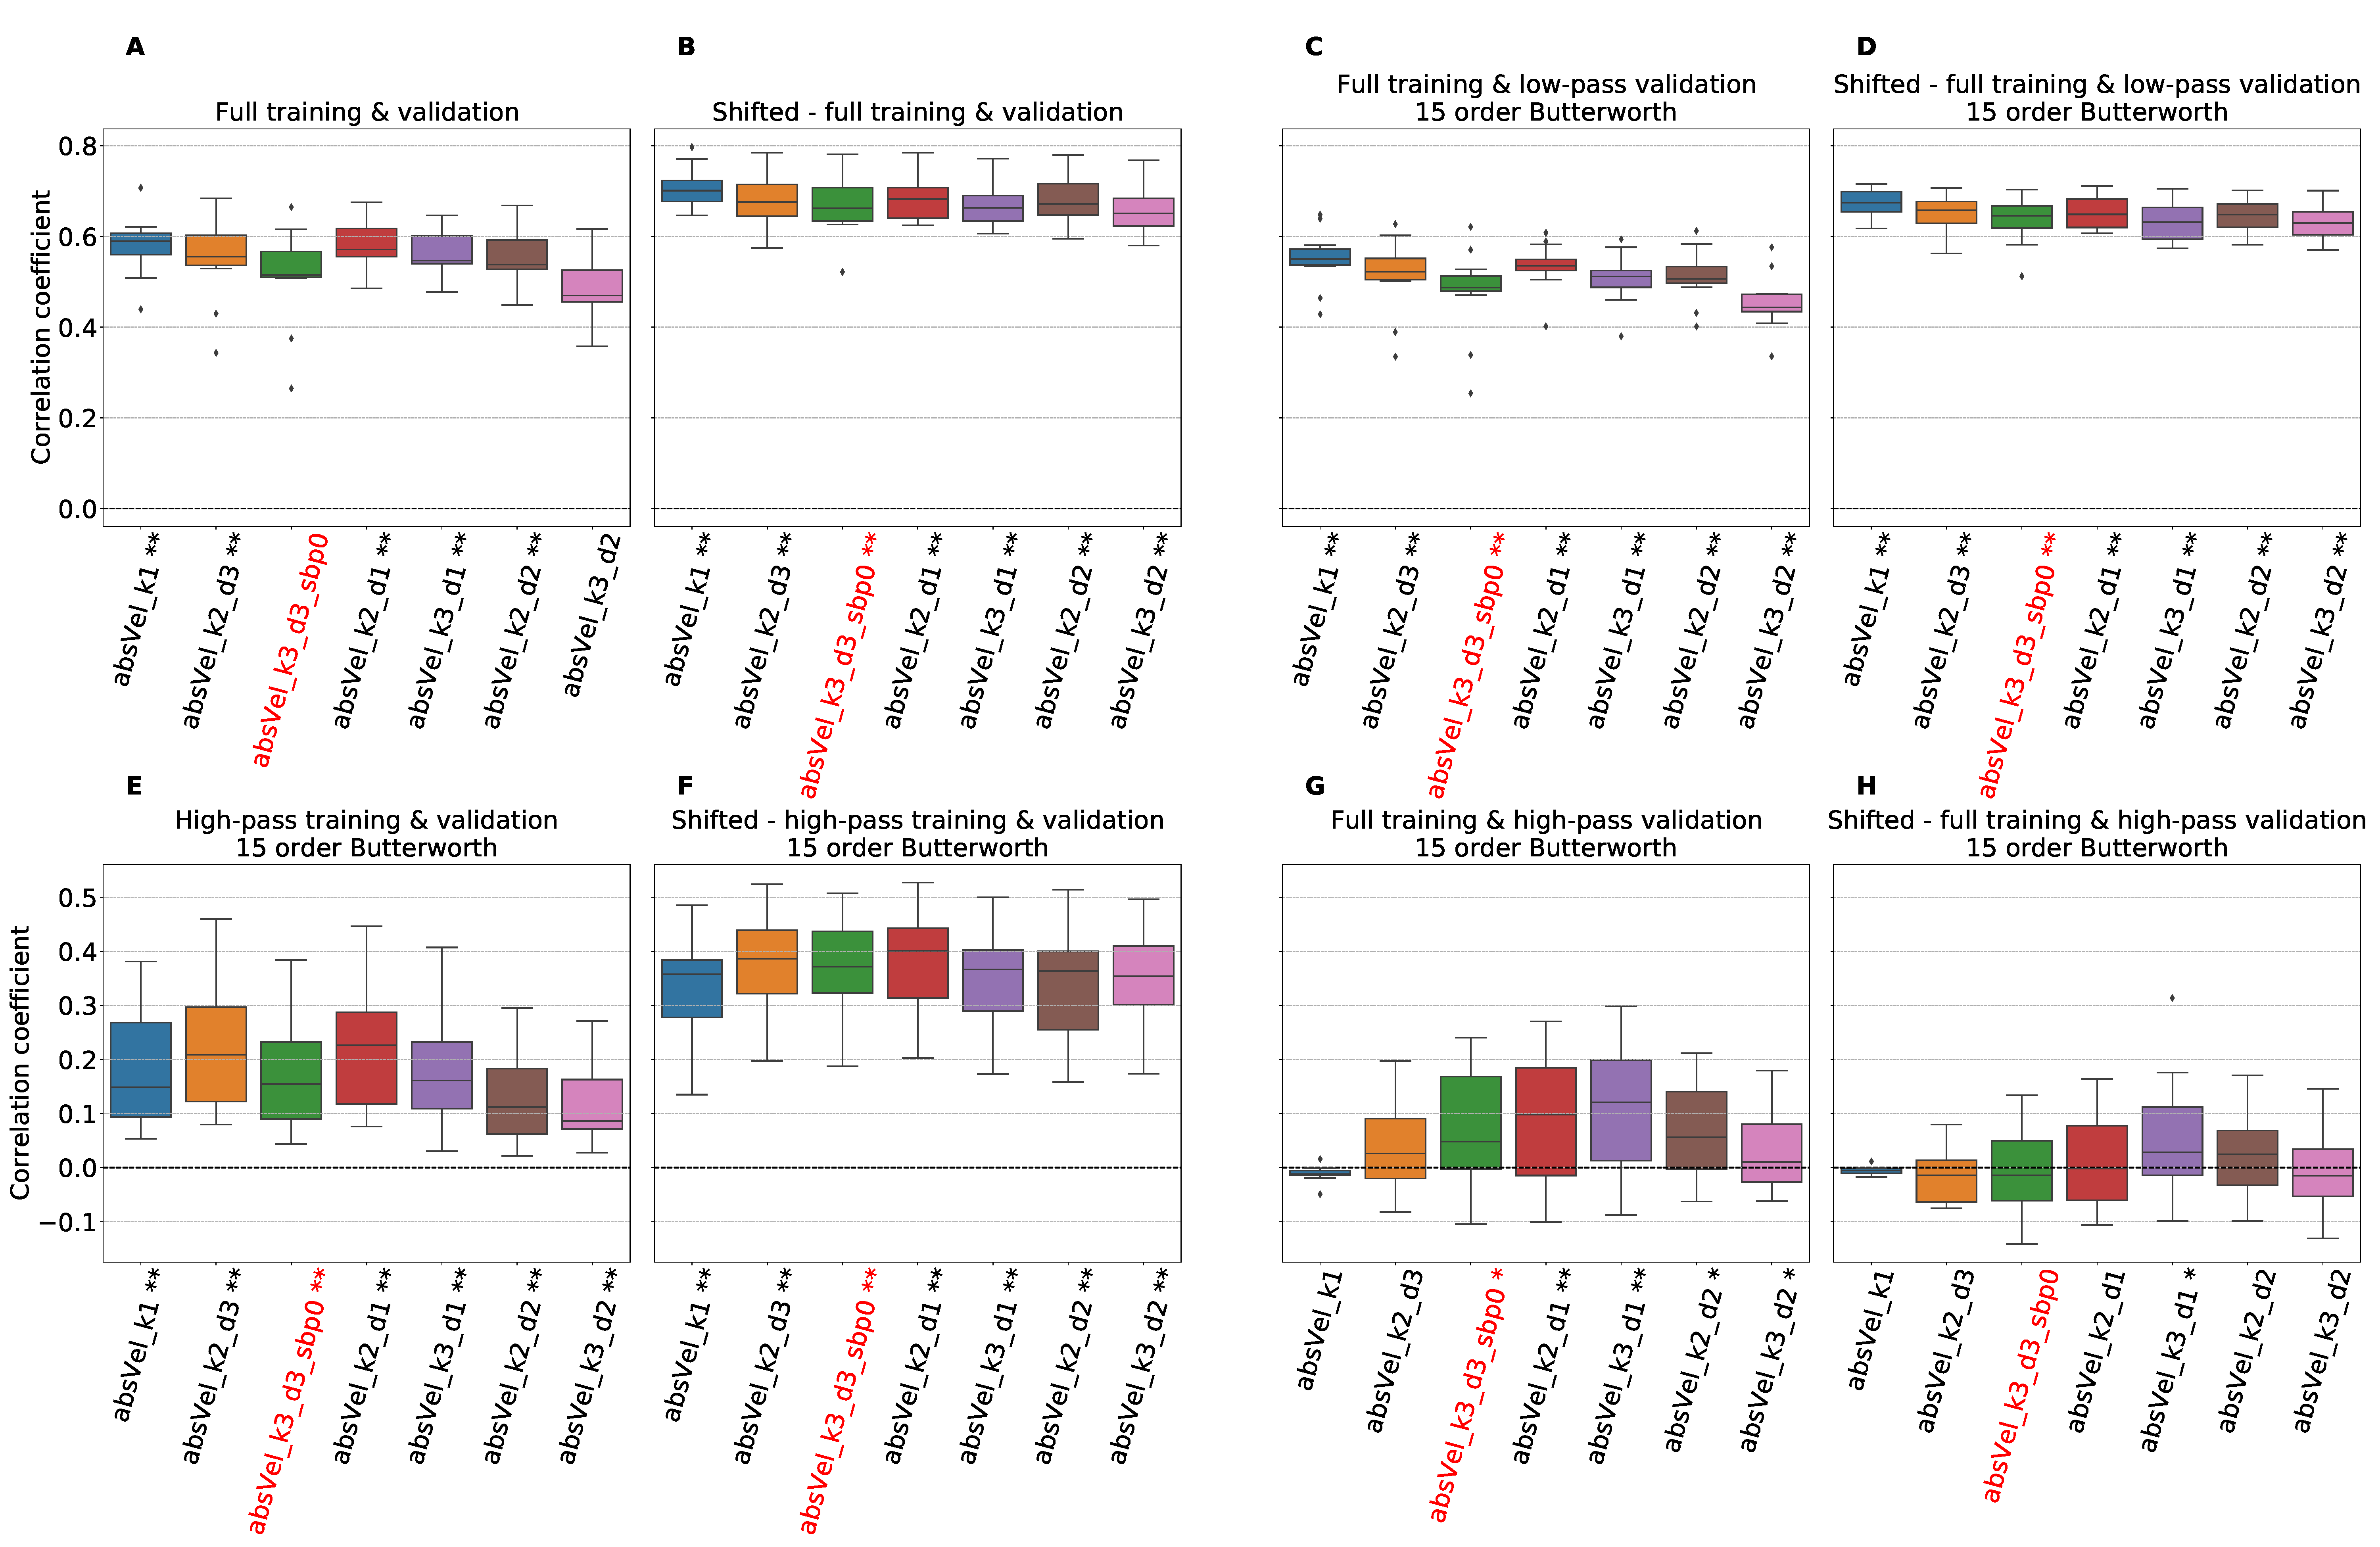
\includegraphics[width=1\linewidth]{img/ch4/shifted_vs_non_shifted_absVel_performance_comparison}
   \caption{}
\end{subfigure}\label{fig:shifted-performance-absVel}
\caption[]{}
\end{figure}\label{fig:shifted-performance}

The improvement can be caused by two things:
\begin{enumerate}
    \item By the network being able to focus on signals recorded directly before the movement execution.
    \item By the network having access to information from the future.
\end{enumerate}

We hypothesise that is most likely a combination of the two.
Conclusion about how much each of the above described influences the prediction improvement cannot be made from the presented experiments.
It would be interesting to build a network with a uniform receptive field and then conduct experiments which would clarify this.
Nevertheless, such an analysis is out of the scope of this thesis.

\subsubsection{Gradients}
In Section~\ref{subsec:gradinet-visualization} we already saw that the best performing networks are those which use lower frequencies.
Here we show, how the shift influences the gradients.
Hypothetically, the information about the movement in high-gamma could be informative only in the moments directly preceding the movement.
Therefore the networks are unable to use it because they focus on the signal recorded too far in the past.
To test this hypothesis, we visualize the gradients of the networks trained in the shifted settings.

We compare the gradients between the networks in the original non-shifted setting and the shifted setting where the predicted time point is in the centre of the receptive field.
This was analysis was performed for all the architectures for all their intermediate layers on 1. the full dataset and 2. the high-passed dataset.
The complete results can be found in the Appendix.
Here, we show results from the third convolutional layer which servers as good representation of the overall trend~\ref{fig:}
The trends are different for the full dataset and the high-passed dataset.

\begin{enumerate}
    \item Gradients of networks which are \textbf{trained and validated on full data} are displayed in Figures~\ref{fig:vel-shifted-vs-non-shifted-grads} and \ref{fig:absVel-shifted-vs-non-shifted-grads}.
    What we observe is that the networks across all architecture seem to refine their focus to more narrow frequency bands.
    For example the vel\_k1 network which is the one without max-pools has high-gradient values in the original setting for frequencies up to 25Hz when looking at gradients for motor channels.
    In the shifted setting the band with high gradient values narrows to frequencies closer to 0.
    The network vek\_k2\_d2 is in the non-shifted setting focused mostly on frequencies between 25 and 60 Hz. Nevertheless, with shifting the gradients for a lot of frequencies the width of the band is reduced, and the network focuses on frequencies around 25Hz. For no network did the shift cause an increase in the use of information from the high-gamma frequency band.
    Rather it seems, that the shift allowed access to less noisy information in the clearly informative bands such as the alpha and beta bands, and the network did not have to compensate with information from other frequencies.
    \item Networks which were \textbf{trained and validated on high-passed data} can be found in Figure \ref{}.
    Again, we only chose to display gradients of one layer to illustrate a behaviour shared by all layers. The gradients of the remaining layers can be found in Appendix \ref{}.
    What we observe in the gradients of the networks trained on high-passed datasets is different from what we observe on gradients of networks trained on full datasets, maybe even the opposite.
    The networks trained on shifted data exhibit interest in the same or a broader range of frequencies above the 60Hz cut-off frequency than the networks trained in the original, non-shifted setting.
    This and the increase in performance on high-passed datasets suggests that indeed the information from the future or directly preceding the movement contains more information about movement in the high-gamma band.
    But the fact that the networks trained on full data do not use high-gamma, and their performance increases significantly compared to the non-shifted setting points to the information in high-gamma being informative but redundant when having access to information from all frequencies.
\end{enumerate}

\begin{figure}[!htpb]
\centering
\RawFloats
\begin{subfigure}[b]{\textwidth}
   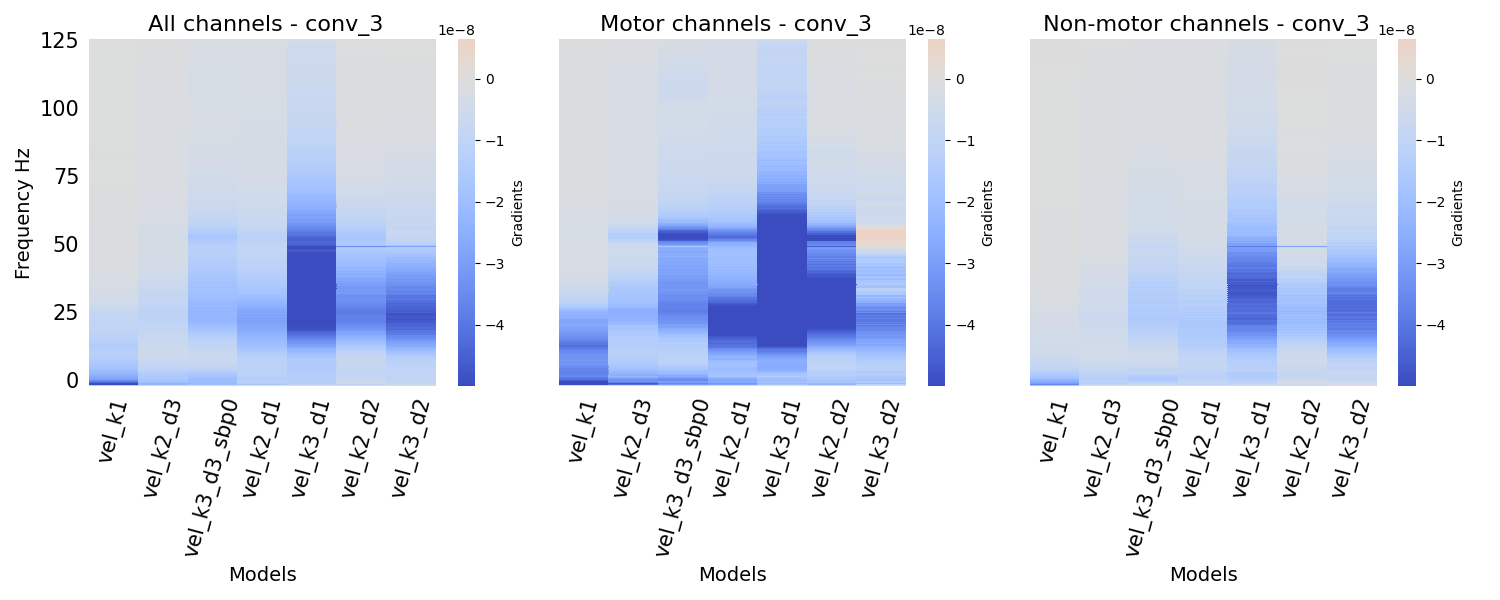
\includegraphics[width=1\linewidth]{img/ch4/vel-conv-3-layer-grads}
   \caption{}
\end{subfigure}\label{fig:vel-conv3-layer-grads}

\begin{subfigure}[b]{\textwidth}
   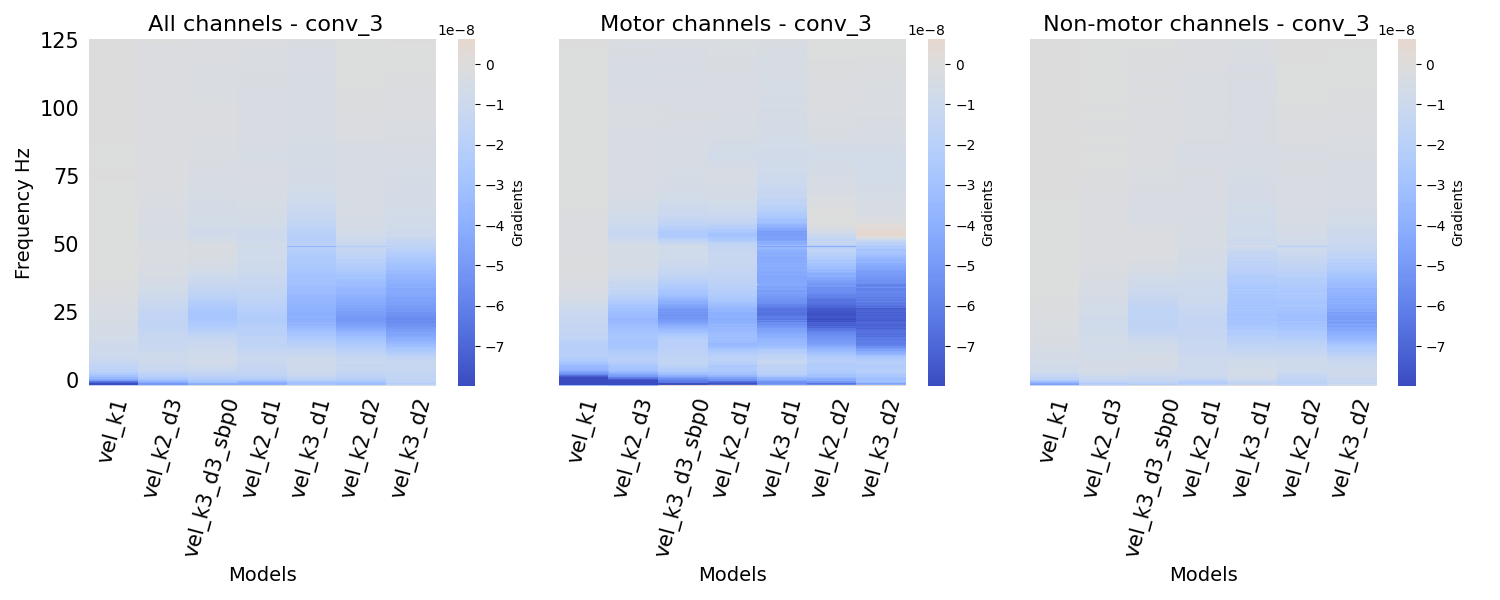
\includegraphics[width=1\linewidth]{img/ch4/vel-conv-3-layer-grads-shifted}
   \caption{}
\end{subfigure}\label{fig:vel-conv3-layer-grads-shifted}
\caption[]{}
\end{figure}\label{fig:vel-shifted-vs-non-shifted-grads}

\begin{figure}[!hpbp]
\begin{subfigure}[a]{\textwidth}
   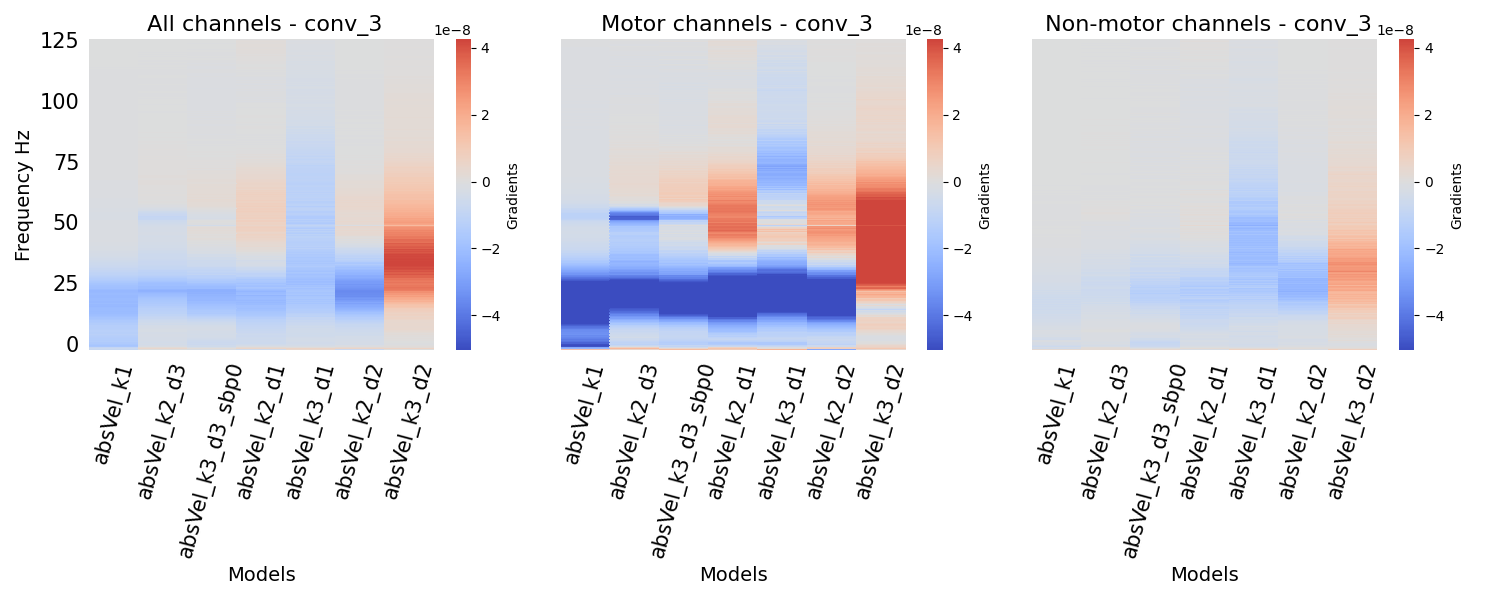
\includegraphics[width=1\linewidth]{img/ch4/absVel-conv-3-layer-grads}
   \caption{}
\end{subfigure}\label{fig:absVel-conv-3-layer-grads}

\begin{subfigure}[b]{\textwidth}
   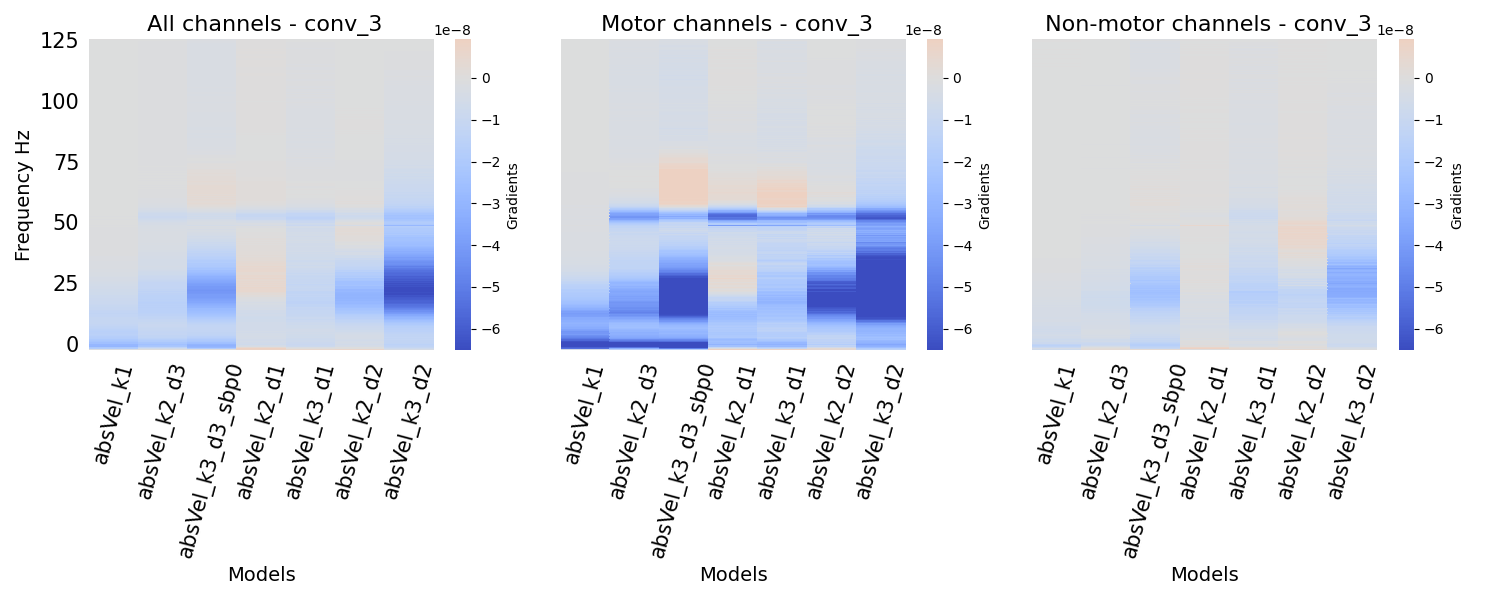
\includegraphics[width=1\linewidth]{img/ch4/absVel-conv-3-layer-grads-shifted}
   \caption{}
\end{subfigure}\label{fig:absVel-conv-3-layer-grads-shifted}
\caption[]{}
\end{figure}\label{fig:absVel-shifted-vs-non-shifted-grads}

% high-pass gradients with shift
\begin{figure}[!htpb]
\centering
\RawFloats
\begin{subfigure}[b]{\textwidth}
   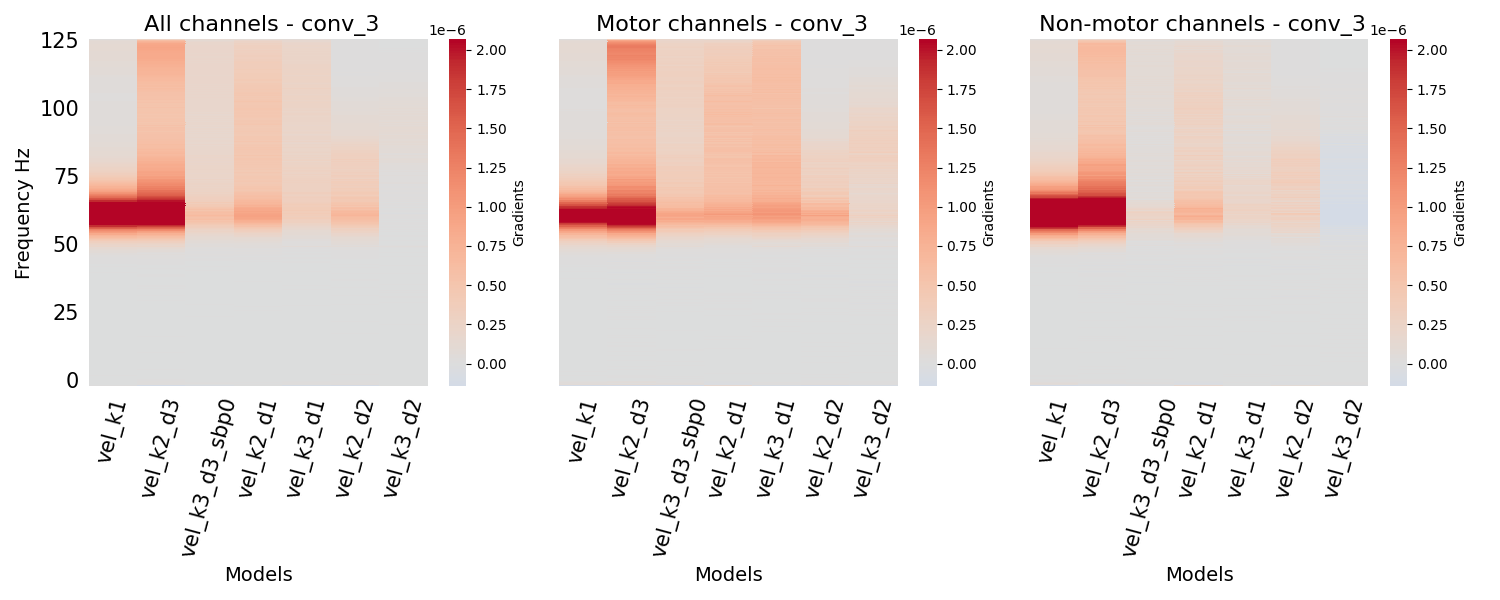
\includegraphics[width=1\linewidth]{img/ch4/vel-conv-3-layer-grads-hp}
   \caption{}
\end{subfigure}\label{fig:vel-conv3-layer-grads-hp}

\begin{subfigure}[b]{\textwidth}
   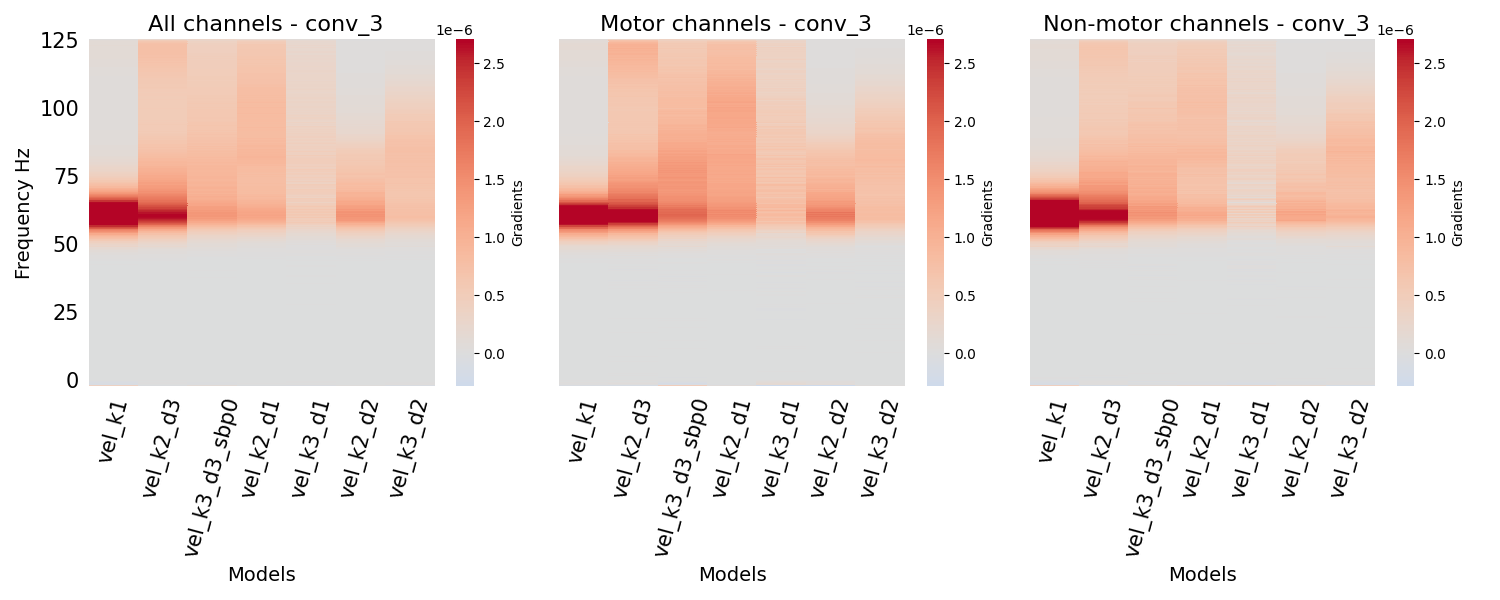
\includegraphics[width=1\linewidth]{img/ch4/vel-conv-3-layer-grads-hp-shifted}
   \caption{}
\end{subfigure}\label{fig:vel-conv3-layer-grads-shifted-hp}
\caption[]{}
\end{figure}\label{fig:vel-shifted-vs-non-shifted-grads-hp}

\begin{figure}[!hpbp]
\begin{subfigure}[a]{\textwidth}
   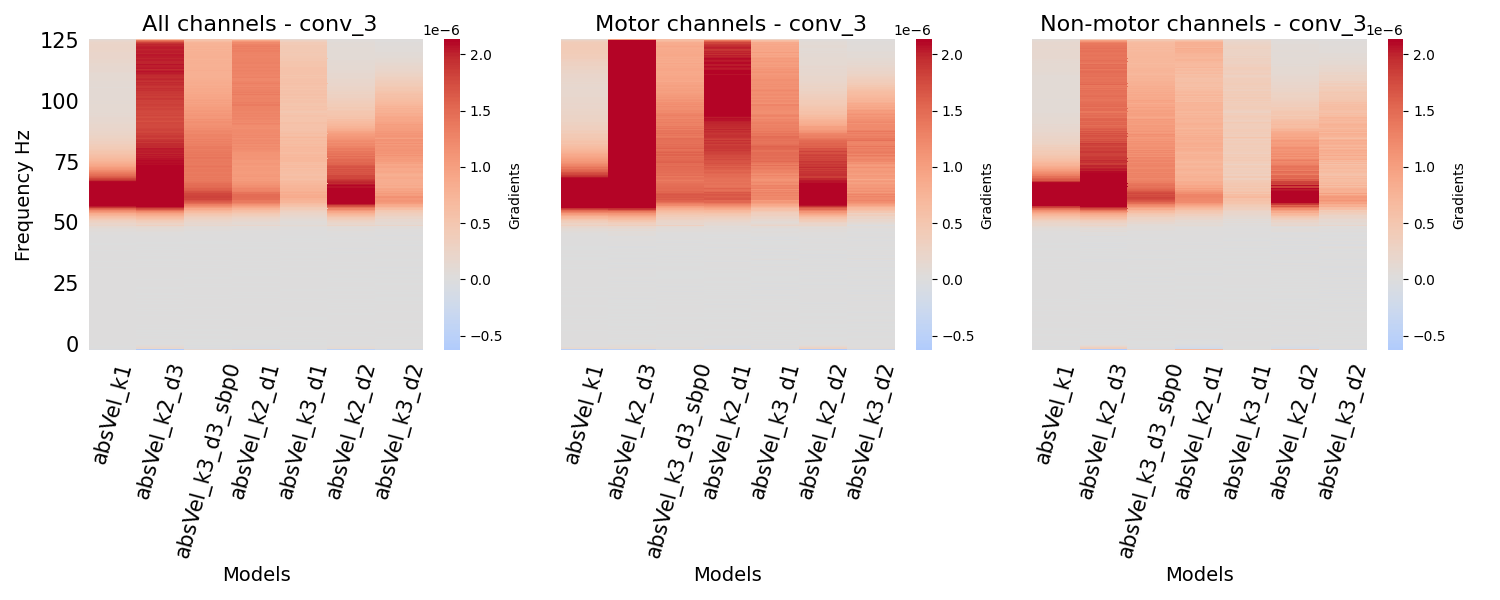
\includegraphics[width=1\linewidth]{img/ch4/absVel-conv-3-layer-grads-hp}
   \caption{}
\end{subfigure}\label{fig:absVel-conv-3-layer-grads-hp}

\begin{subfigure}[b]{\textwidth}
   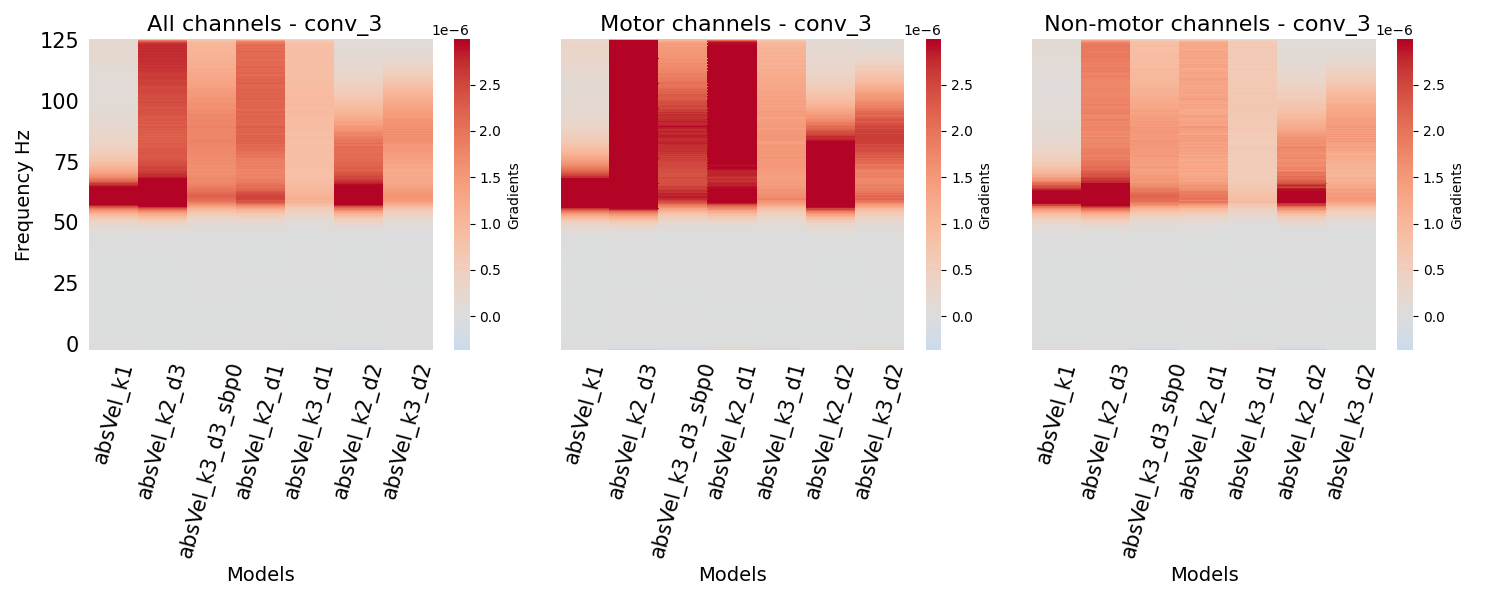
\includegraphics[width=1\linewidth]{img/ch4/absVel-conv-3-layer-grads-hp-shifted}
   \caption{}
\end{subfigure}\label{fig:absVel-conv-3-layer-grads-shifted-hp}
\caption[]{}
\end{figure}\label{fig:absVel-shifted-vs-non-shifted-grads-hp}

\subsubsection{Summary}\label{subsubsec:centre-shiftig-summary}
When looking at the performances and gradients of the various CNN architectures, the following observation can be made.
\begin{itemize}
    \item The shift improves performance 1. when training and validating on the full dataset; 2. when training on the full dataset and validating on low-passed data;
    3. when training and validating on high-passed data. This is true for both velocity and absolute velocity.
    \item The shift attenuates the differences in performance between the different CNNs for the full training and validation.
    When looking at graphs \textbf{B} in both~\cref{fig:shifted-performance-vel} and~\cref{fig:shifted-performance-absVel}, we can see that the number of network which have a significantly better performance than the original Deep4Net (k3\_d3\_sbp0) decreases compared to \textbf{A}.
    \item The shift does not improve performance for the CNNs trained on full data and validated on high-pass data (graphs \textbf{G} and \textbf{H} in both~\ref{fig:shifted-performance-vel} and~\ref{fig:shifted-performance-absVel}).
    This result together with the more narrow frequency bands the networks focus on after the shift show, that opposite to the expectation, the networks do not start focusing on high-gamma with the shift.
    They start to focus more on information from the lower frequency bands which.
    Modulations in these low frequency bands become more informative with the shift, therefore the performance increase, and the interest of the CNNs in higher frequencies drops.
    \item It is true in the shifted setting, as was in the non-shifted setting, that the network without max-pool (k1) which is most solely focused on low-frequency modulations performs the best.
    \item The modulations in the high-gamma band also become more informative for decoding with the shift, thus the increase in performance when training and validating on the high-passed dataset.
    Nevertheless, as we state in the point above, not even this motivates the networks to use information from the high-gamma band.
    The opposite happens.
\end{itemize}

From the observations above, we can state, that the modulations in the high-gamma band are not particularly informative for velocity and absolute velocity decoding.
They contain information the CNNs are able to use for decoding, nevertheless, it is not an advantage for the CNN, rather it harms its performance.
It is better for the CNNs to focus on low frequencies.


\subsection{Shifting the predicted time-point across receptive field}\label{subsec:shifting-the-predicted-time-point-across-receptive-field}
Besides the big shift from the edge of the receptive field to the centre we also studied what happens if we shift the predicted time-point in smaller steps across the receptive field of the network. 
The shifts are made ranging from  -1 s  to 1 s with respect to the receptive field centre which we denote as 0.
The step size was 0.1 s which is equivalent to 25 samples.
This way, we can observe how the shifting gradually influences the performance and gradients of the network. 

Unlike the previous experiments we chose to perform this analysis only on one architecture, namely, the Deep4Net\_sbp0. 
The shift seems to influence the gradients of all the networks similarly.
And therefore, the amount of time and computational power necessary to train multiple networks for each time-steps seems excessive.  

\subsubsection{Performance}\label{subsubsec:across-shiftig-performace}
The performance gradually changing with the shift is displayed in Figure~\ref{fig:shifting-performance}.
We can observe the slow decrease in performance when increasing the distance of the predicted time-point to the receptive field centre, in both directions. 
This is to be expected. 
Nevertheless, similarly to performance in section~\ref{subsec:shifting-the-predicted-time-point-to-the-centre-of-the-receptive-field} we do not know if the fact that the performance peaks in the centre of the receptive field is due to the predicted time-point being in the centre of the receptive field.
It could again also be due to the fact that the network has information from the future. 
Interestingly, the decoding performance drops slower when using information predominantly from the future more than when using information predominantly from the past.
To properly investigate the informativeness of past vs. future signals however, we would need to have a network with an uniform receptive field. 
\todo{some literature about this}.

\begin{figure}[!hpbp]
\begin{subfigure}[a]{\textwidth}
   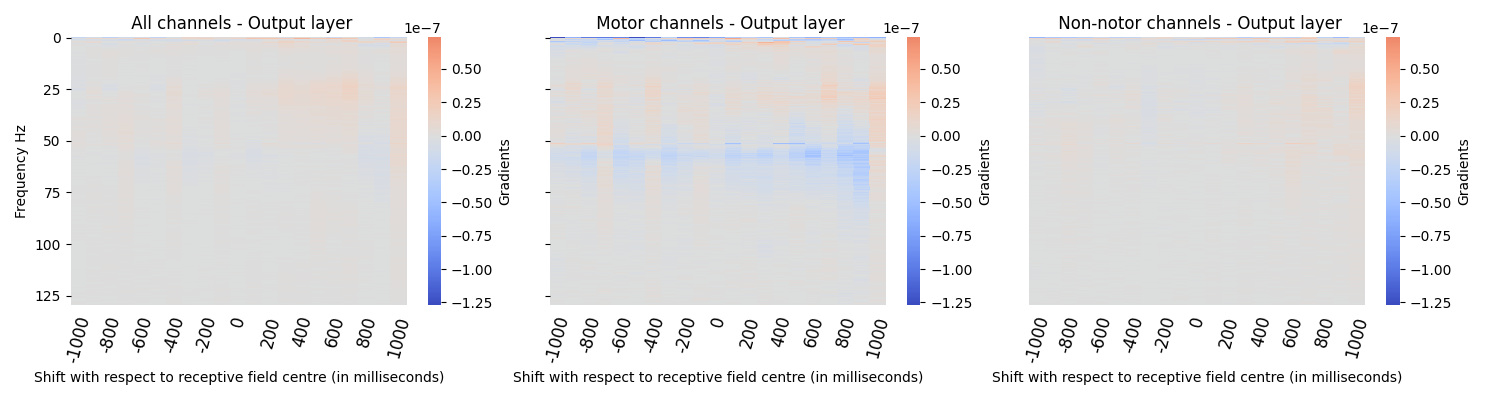
\includegraphics[width=1\linewidth]{img/ch4/vel-shifted-gradients}
   \caption{}
\end{subfigure}\label{fig:vel-shifting-performance}

\begin{subfigure}[b]{\textwidth}
   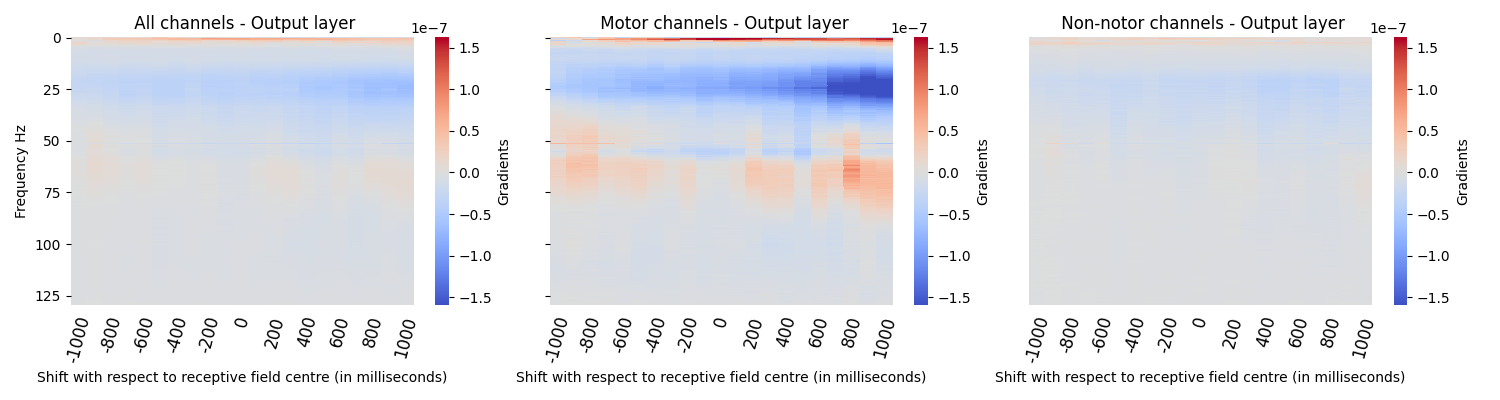
\includegraphics[width=1\linewidth]{img/ch4/absVel-shifted-gradients}
   \caption{}
\end{subfigure}\label{fig:absVel-shiftig-performance}
\caption[]{}
\end{figure}\label{fig:shifting-performance}

Besides observing how performance changes with shifting, we also visualize the gradients as is described in the next section.

\subsubsection{Gradients}\label{subsubsec:across-shiftig-gradients}
The gradients are visualized in Figure~\ref{fig:shifting-performance}.
In the graph for absolute velocity, we can observe the trend of broadening the frequency ranges with high gradient values when shifting the predicted time-point from the centre of the receptive field both to the left and to the right.
This is what we expected because it corresponds to the results from~\cref{subsec:shifting-the-predicted-time-point-to-the-centre-of-the-receptive-field}.
Interestingly, when plotting the same graph for velocity, we do not observe this behaviour so clearly, instead there is a periodicity in the positive and negative value of the gradients for the different values of the shift.
It is unclear why this periodicity occurs.


\subsubsection{Summary}\label{subsubsec:across-shiftig-summary}
Besides the periodicity of the positive and negative values of the gradients in for velocity, we have further confirmed the conclusions we drew previously in \ref{subsec:shifting-the-predicted-time-point-to-the-centre-of-the-receptive-field}. 
Indeed the network seems to focus on more narrow frequency bands when given better access to information close to its receptive field.
In the case of the Deep4Net\_spb0 it also means lower interest in the high-gamma frequency band when achieving better performance.
This corroborates the what we have established so far about the information in the high-gamma band being inferior for velocity and absolute velocity decoding compared to information from lower frequency bands. 


\section{Spectral whitening}\label{sec:spectral-whitening}


\subsection{Performance}\label{subsec:pw-performance}
How the networks react to datasets which were whitened as described in Section~\ref{subsec:modifications-to-the-dataset} was one of our interests because when we look at the spectrum of the original signal, the amplitudes of frequencies decrease exponentially with increase in the frequency.
This is common in biological signals but could be a reason for the network to ignore high-frequencies when making predictions. Figure~\ref{pw-performances-full-data} shows how the predictions changed compared to predictions on non-whitened signals when using the full dataset.
It is obvious that the correlation coefficient of all networks dropped significantly.
When looking at Figure~\ref{fig:pw-performance} graphs we see that in the case of high-passed datasets the decrease was lower, but even for the high-passed data, the performance did not increase.

\begin{figure}[!hpbp]
\begin{subfigure}[a]{\textwidth}
   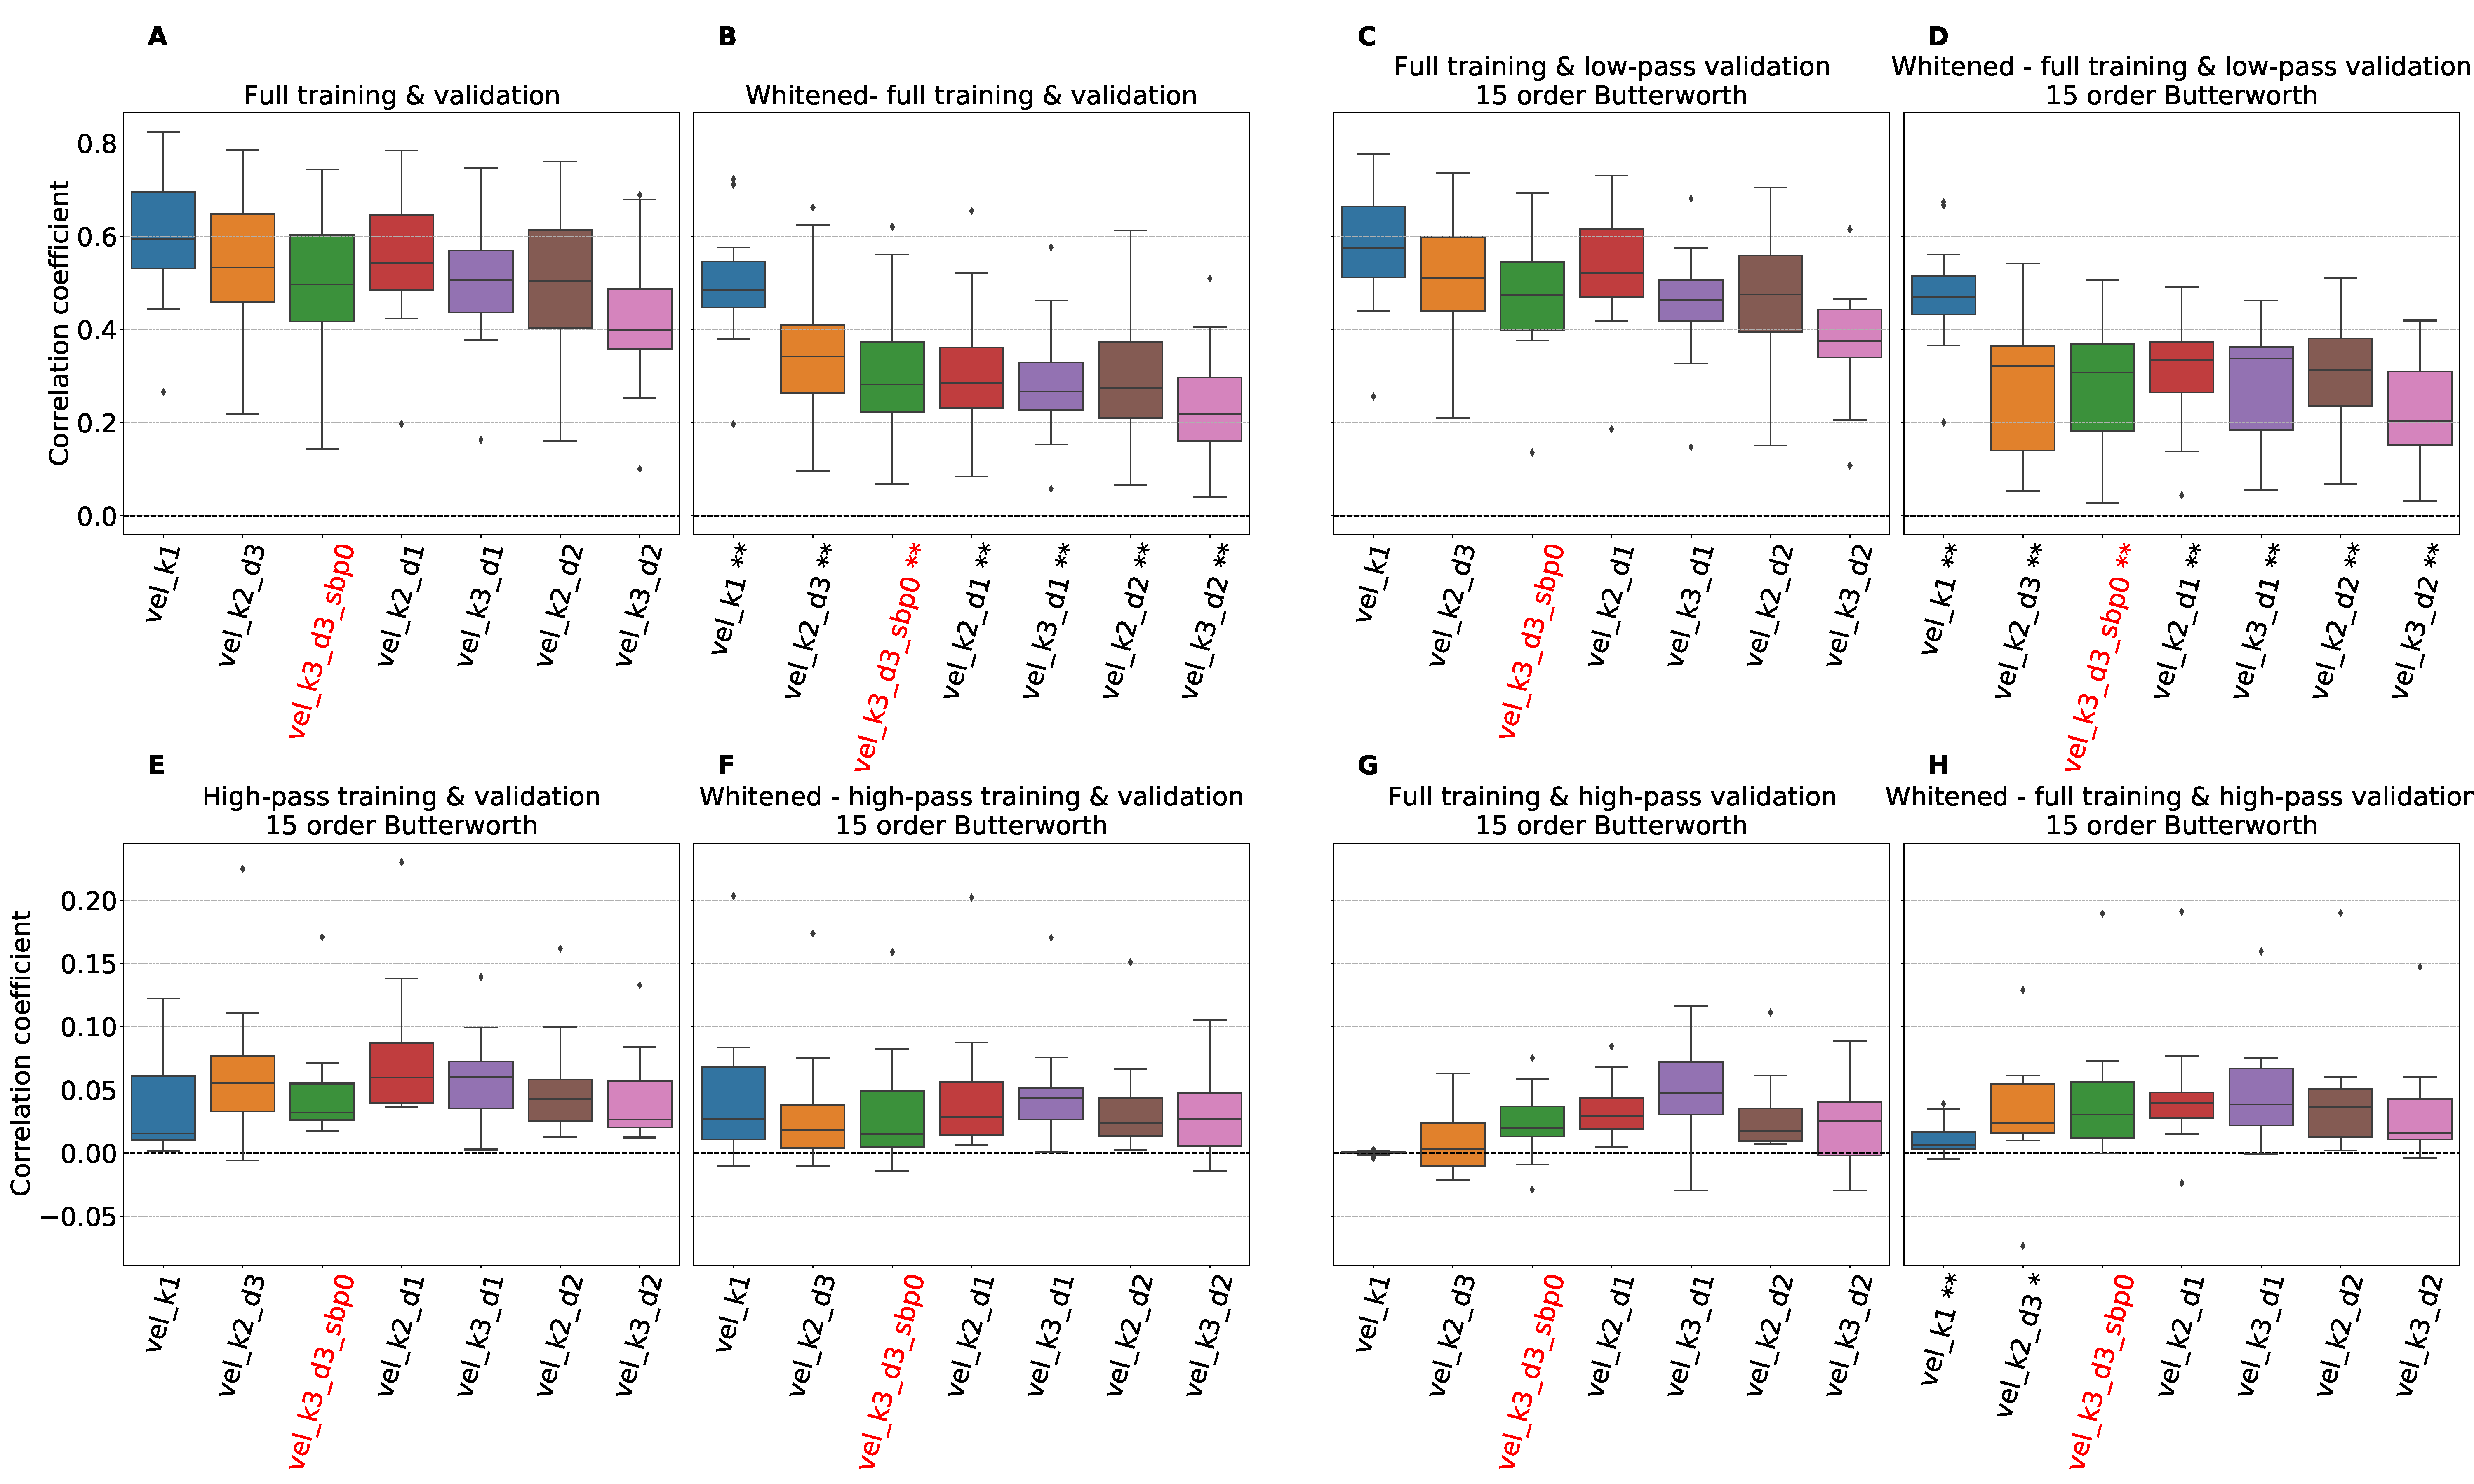
\includegraphics[width=1\linewidth]{img/ch4/vel-pw-vs-non-pw-performance}
   \caption{}
\end{subfigure}\label{fig:vel-pw-performance}

\begin{subfigure}[b]{\textwidth}
   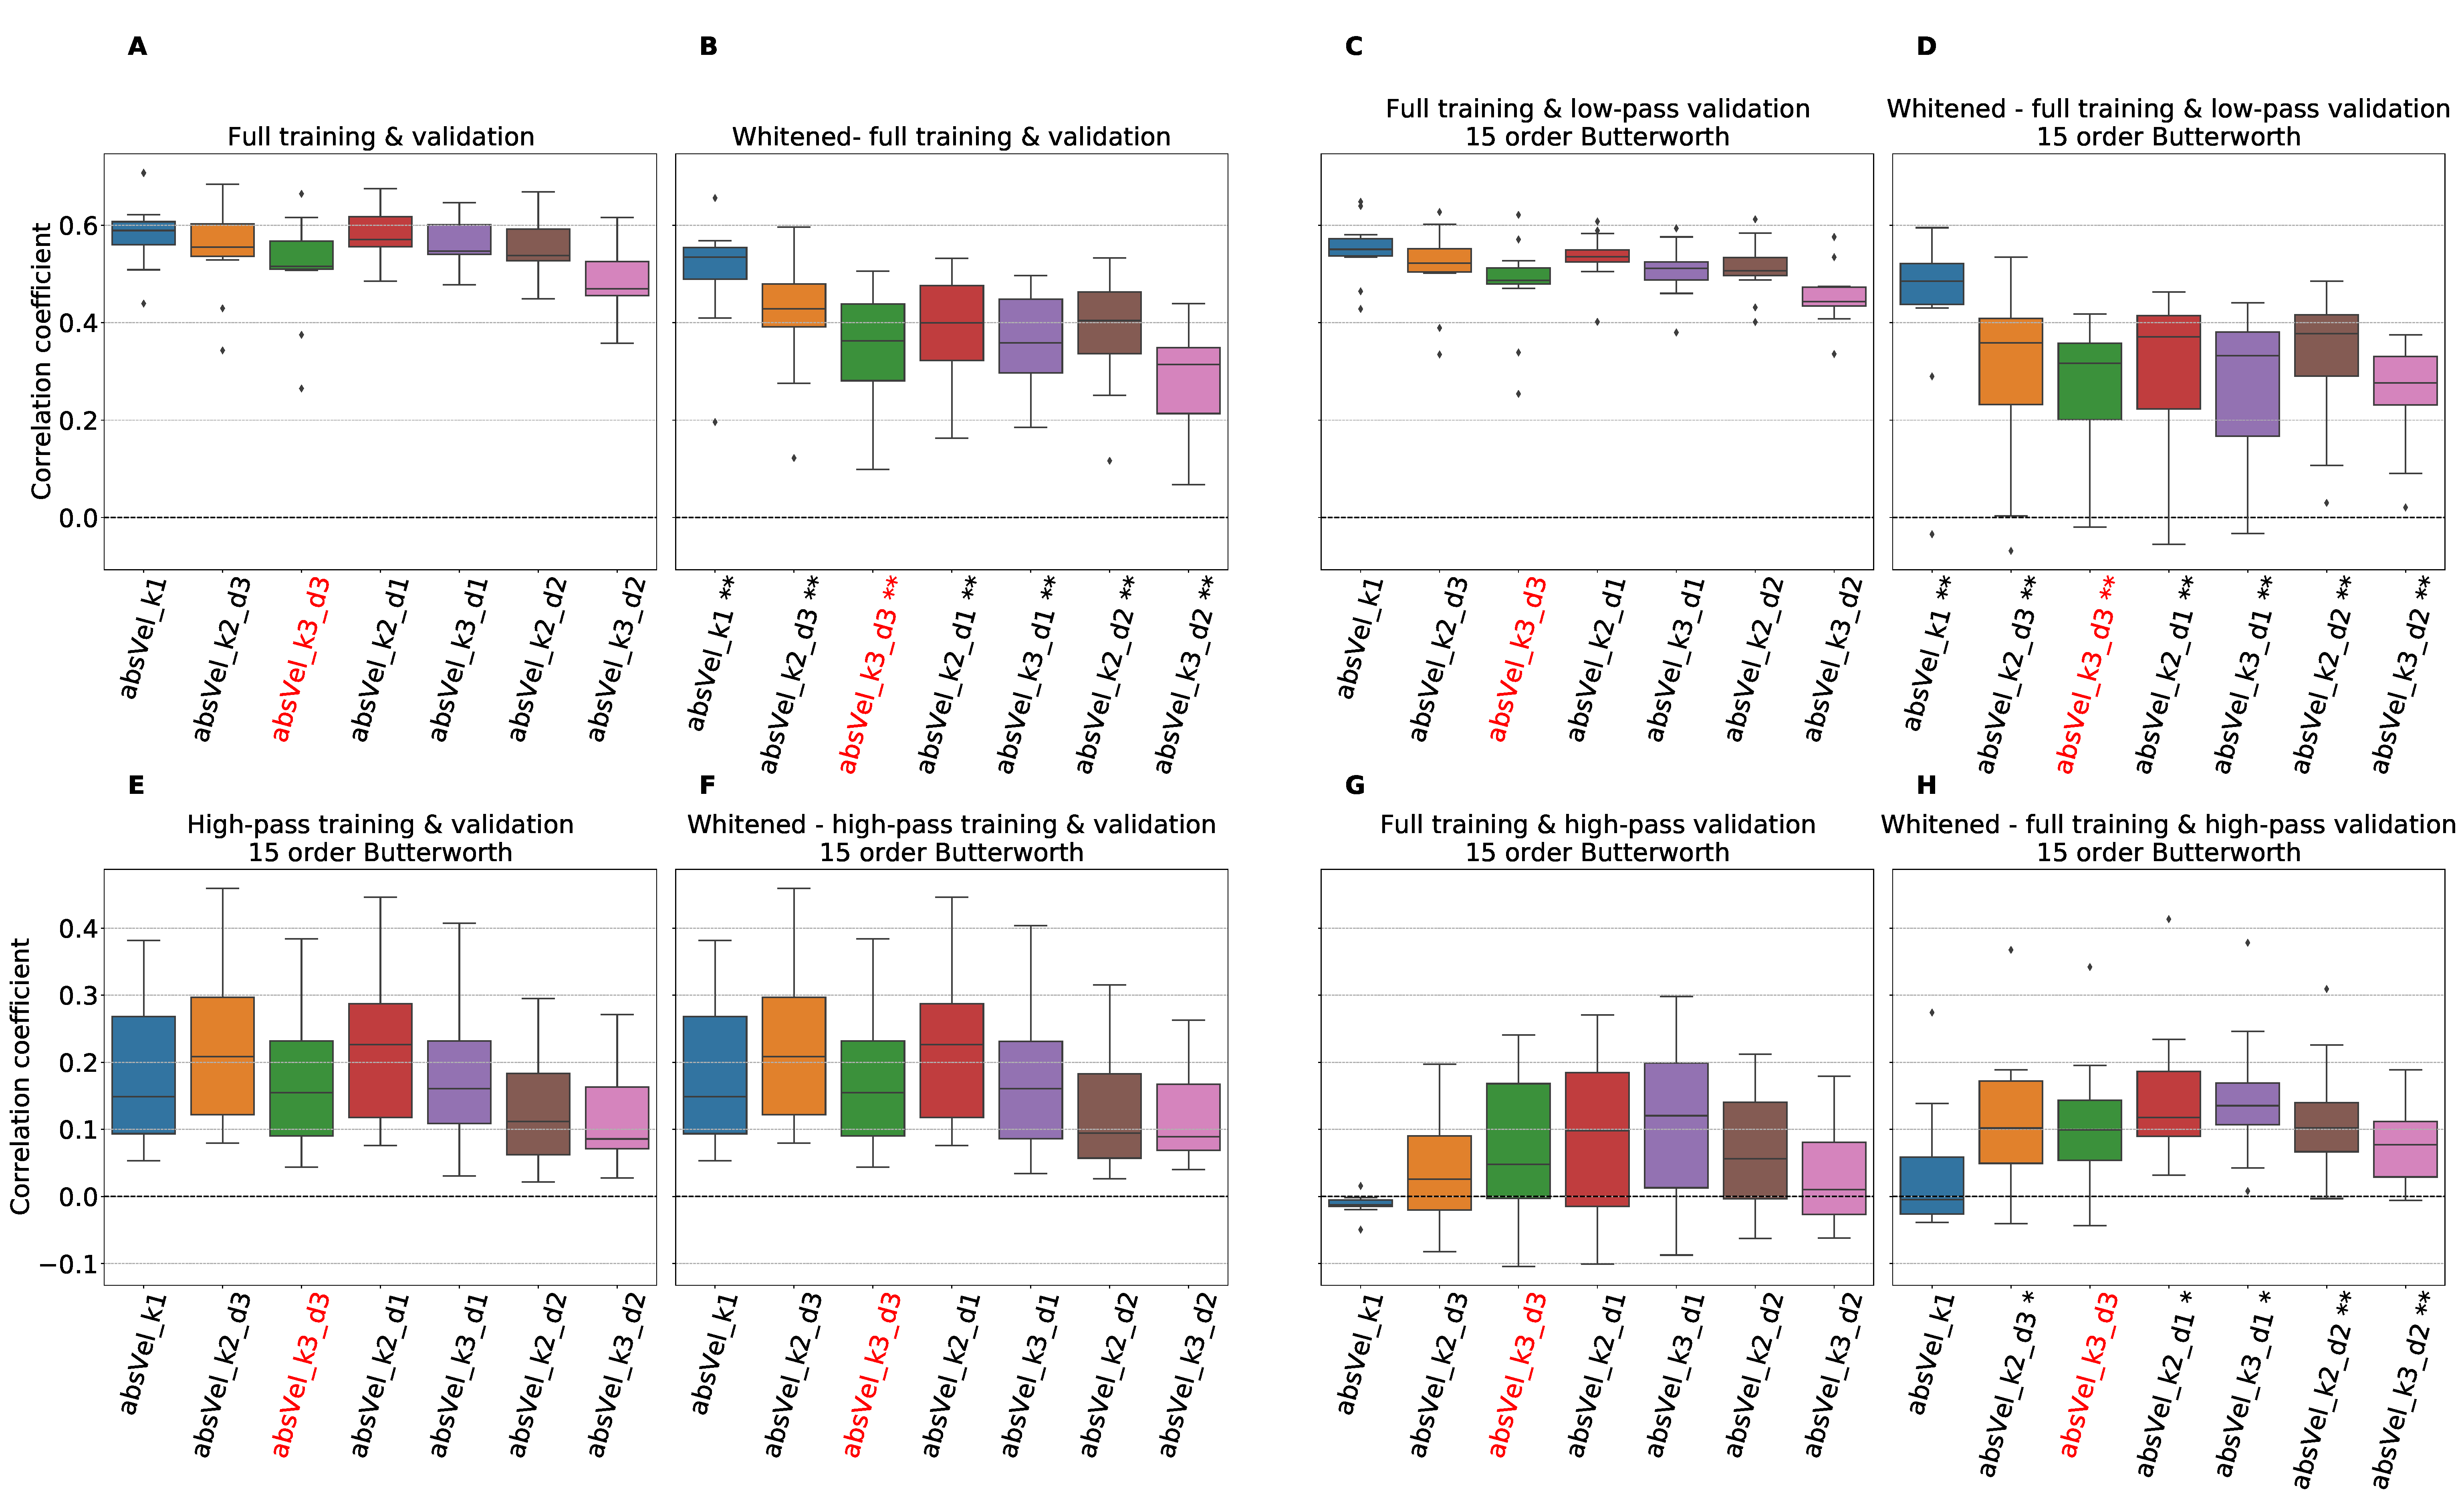
\includegraphics[width=1\linewidth]{img/ch4/absVel-pw-vs-non-pw-performance}
   \caption{}
\end{subfigure}\label{fig:absVel-pw-performance}
\caption[]{}
\end{figure}\label{fig:pw-performance}

\subsection{Gradients}\label{subsec:pw-gradients2}

When looking at the gradients of the networks trained on whitened data, we observe that the networks indeed use modulations in the high-gamma frequency bands for their predictions.
Interestingly instead of having uniform gradients across all frequencies, they inverted their focus from low frequencies to high-frequencies.
The only architectures for which this did not happen are the models vel\_k1 and absVel\_k1 which are the networks without a max-pool layer.
When looking at the performance graphs in Figure~\ref{fig:pw-last-layer-grads} though, these are the networks for which the performance dropped least.
This again suggests that the using information from the high-gamma frequency is possible, but it does not seem to help achieve better correlation coefficients.

\begin{figure}[!hpbp]
\begin{subfigure}[a]{\textwidth}
   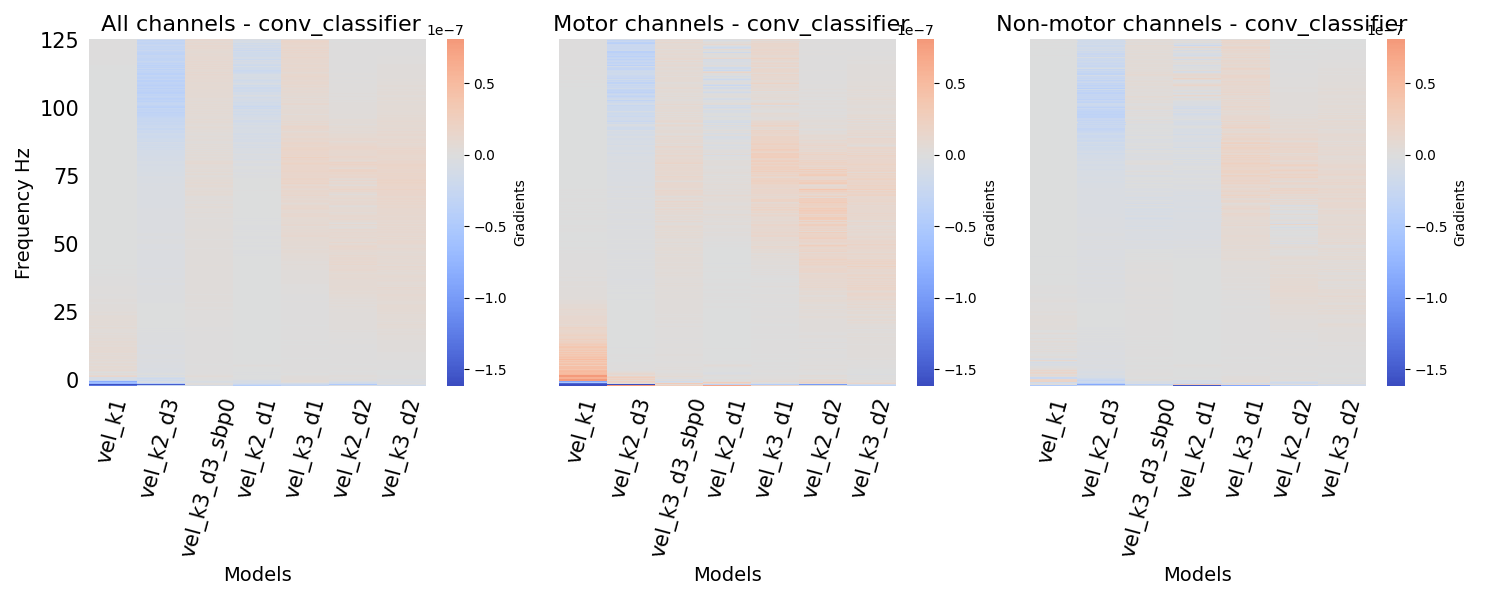
\includegraphics[width=1\linewidth]{img/ch4/vel-pw-last-layer-grads}
   \caption{}
\end{subfigure}\label{fig:vel-pw-last-layer-grads}

\begin{subfigure}[b]{\textwidth}
   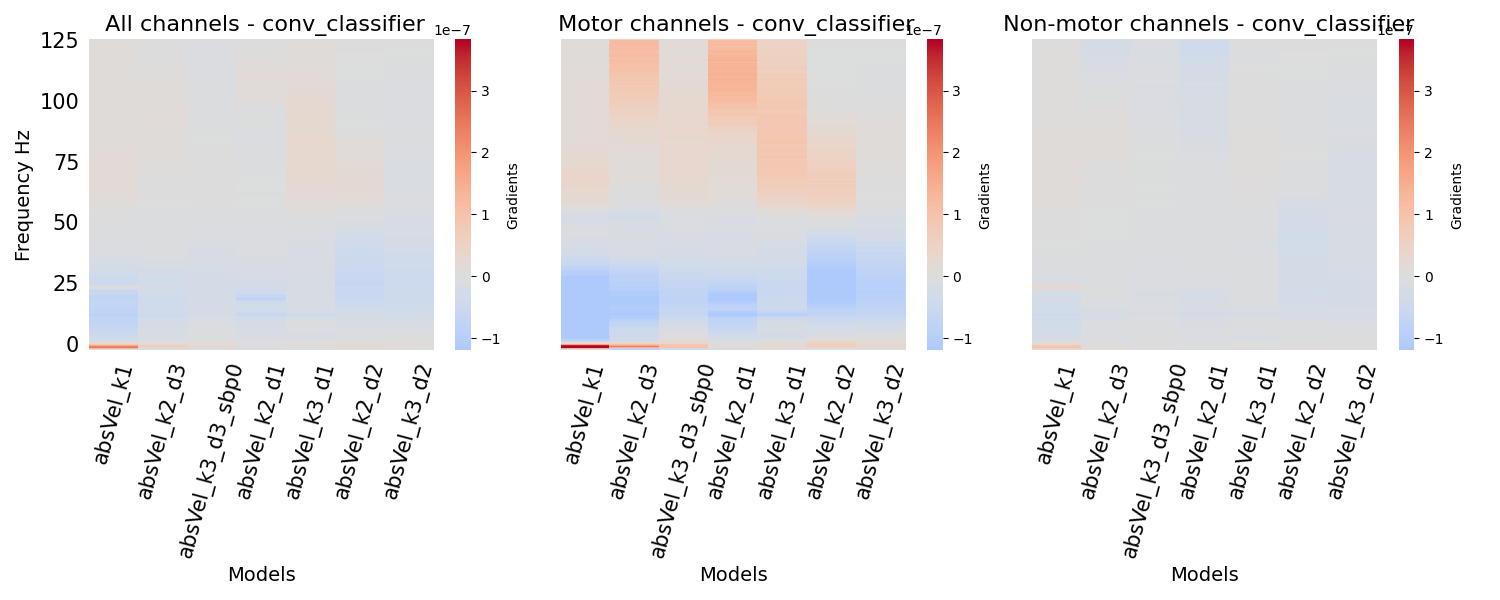
\includegraphics[width=1\linewidth]{img/ch4/absVel-pw-last-layer-grads}
   \caption{}
\end{subfigure}\label{fig:absVel-pw-last-layet-grads}
\caption[]{}
\end{figure}\label{fig:pw-last-layer-grads}

\subsection{Summary}\label{subsec:pw-summary}

\chapwithtoc{Conclusion}

A deeper understanding of which iEEG features CNNs use for movement decoding broadens our understanding of how the brain encodes movement related information.
It also partially alleviates the \textit{black box} problem associated with deep neural networks.
Improvement of performance of such networks makes them more perspective for real-life clinical applications.
The work of \cite{Hammer-2021} offers both performance improvement and a deeper understanding of which features are crucial for the CNN to make predictions.
Nevertheless, their findings also raise some questions.
Mainly the low importance of the high-gamma frequency band for absolute velocity decoding challenges previous findings about its informativeness for absolute velocity decoding (\cite{hammer-predominance-2016}).
The main goal of the thesis was to further study the frequency bands utilized by the Deep4Net with particular focus on the high-gamma frequencies and to identify modifications to the CNN architecture which improves utilization of information across useful frequency bands. \\

The contributions of this thesis are following:
\begin{itemize}
    \item We showed that the high-gamma frequency band contains information relevant for movement decoding, especially for absolute velocity decoding. Nevertheless, its usage does not improve performance. On the contrary, its usage correlates with worse prediction when having access to all frequencies.
    \item We have identified the pooling layers in the architecture of the Deep4Net as unnecessary. Their removal optimizes information extraction from low frequency bands and improves overall performance of the CNN.
    \item We have identified the non-uniformity of the receptive field as a potential drawback of the architecture. It causes the CNN to be biased towards signals relatively far from the predicted time-point.
\end{itemize}


\section*{Main findings}

\subsection*{Informative frequency bands}
Most of the experiments we performed were motivated by making the network use information from the high-gamma frequency band in their prediction.
Building different architectures was motivated by studying a peak in the high-gamma band, shifting the predicted time-point was motivated by the hypothesis, that relevant information is contained in the high-gamma of iEEG signals only directly before movement execution, and spectral whitening was motivated by a difference reduction in the amplitudes of lower vs. higher frequencies because we thought that lower amplitudes of high-frequencies are a disadvantage.
Based on previous literature, the usage of high-gamma especially for absolute velocity decoding seemed like something that should occur.
And because it did not, the idea was that forcing the network to use high-gamma would improve their performance.

Nevertheless, despite the substantial effort to show that high-gamma modulations are informative for velocity and absolute velocity decoding, the results repeatedly show that the Deep4Net and similar CNN architectures do not benefit from using high-gamma information when having access to information from all frequency bands.
While we show that the high-gamma frequencies in iEEG contain relevant information especially for absolute velocity decoding, the CNNs profit from not using this information when making predictions.
The most successful architecture, namely the CNN without max-pool layers, was the one least focused on modulations in the high-gamma frequency band.
It was also the network which despite spectral whitening stayed focused mainly on low-frequency modulations and its performance dropped least.
The shift of the predicted time-point to the centre of the receptive field which greatly improved performance also did not cause an increased interest in the high-gamma frequencies of any network.
Rather it refined the focus of the networks to more narrow and mostly also lower frequency bands.

\subsection*{Architecture modifications}
We have identified two main possibilities for architectural improvement of the Deep4Net. 
First, removing the max-pool layers from the architecture improves performance significantly compared to the original Deep4Net. 
Based on the performance evaluation on filtered datasets and the gradient visualization, we find that this modification allows the network to use information from low frequency bands more effectively. 

Secondly, the non-uniformity of the receptive field could be a drawback of the architecture.
It causes the network to consider mostly information which are too far in the past with respect to the predicted time-point.
We hypothesise, that making the receptive field uniform, by allowing padding at least in the direction from the centre of the receptive field towards the predicted time-point, would improve the achieved correlation coefficients.
While the experiments we conducted in this thesis cannot clearly confirm this hypothesis, the performance improvement when shifting the predicted time-point to the centre of the receptive field speaks at least partially in its favor. 

These two findings are useful for designing CNNs for movement decoding in the future.

\section*{Future work}
Our research offers a wide range of future directions.
The most prominent next step would be building a network with a uniform receptive field which would still be useful for on-line BCI and would likely make better predictions.
Further steps could also be taken in studying which frequencies the network uses.
Even though our research was fairly thorough in this regard, there is always more to find.
The signal consist not only from amplitudes of different frequencies but also contains phase information which has been shown to also hold movement related information (\cite{Hammer-2021, hartmann-hierarchical-2018}). 
Thus, a similar analysis of the influence of phase of the different frequencies might be an interesting future project.
And even when considering amplitudes again, besides the high-passed and low-passed datasets, datasets band-passed to only certain, more narrow, frequency bands could be created and the performance and gradients of the networks could be analysed similarly to what we did in our thesis.





\ifEN
\chapwithtoc{Bibliography}
\else
\chapwithtoc{Seznam použité literatury}
\fi

\printbibliography[heading=none]

\listoffigures
\listoftables
\appendix
\chapter{Using CoolThesisSoftware}

Use this appendix to tell the readers (specifically the reviewer) how to use your software. A very reduced example follows; expand as necessary. Description of the program usage (e.g., how to process some example data) should be included as well.

To compile and run the software, you need dependencies XXX and YYY and a C compiler. On Debian-based Linux systems (such as Ubuntu), you may install these dependencies with APT:
\begin{Verbatim}
apt-get install \
  libsuperdependency-dev \
  libanotherdependency-dev \
  build-essential
\end{Verbatim}

To unpack and compile the software, proceed as follows:
\begin{Verbatim}
unzip coolsoft.zip
cd coolsoft
./configure
make
\end{Verbatim}

The program can be used as a C++ library, the simplest use is demonstrated in \cref{lst:ex}. A demonstration program that processes demonstration data is available in directory \verb|demo/|, you can run the program on a demonstration dataset as follows:
\begin{Verbatim}
cd demo/
./bin/cool_process_data data/demo1
\end{Verbatim}

After the program starts, control the data avenger with standard \verb-WSAD- controls.

\begin{listing}
\begin{lstlisting}
#include <CoolSoft.h>
#include <iostream>

int main() {
	int i;
	if(i = cool::ProcessAllData()) // returns 0 on error
		std::cout << i << std::endl;
	else
		std::cerr << "error!" << std::endl;
	return 0;
}
\end{lstlisting}
\caption{Example program.}
\label{lst:ex}
\end{listing}

\chapter{Gradients of all architectures - shifted}\label{appendixB}

\section*{Velocity - Full dataset}\label{sec:velocity-appendixB}

\begin{figure}[!htpb]
\centering
\begin{subfigure}[b]{\textwidth}
   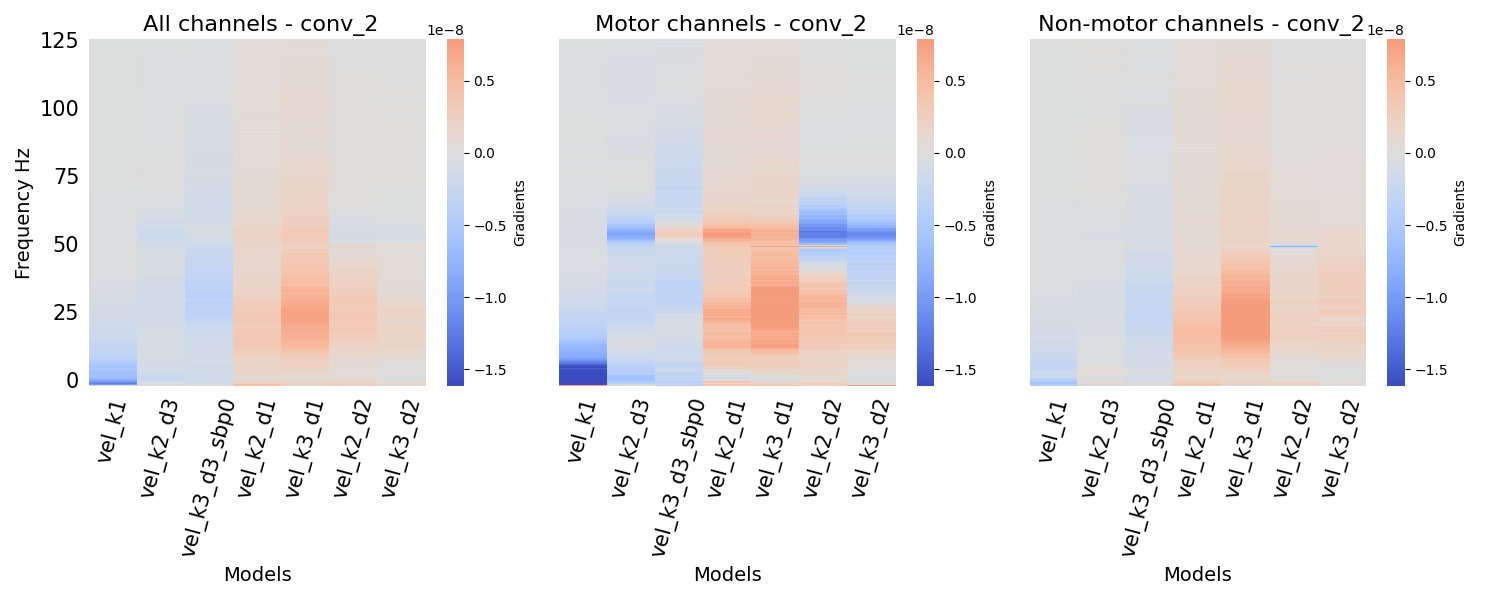
\includegraphics[width=0.85\linewidth]{img/appendix/A/conv-2/sm/vel-model-gradients-all_kinds}
   \caption{}
   \label{fig:vel-shifted-grads-conv-2}
\end{subfigure}

\begin{subfigure}[b]{\textwidth}
   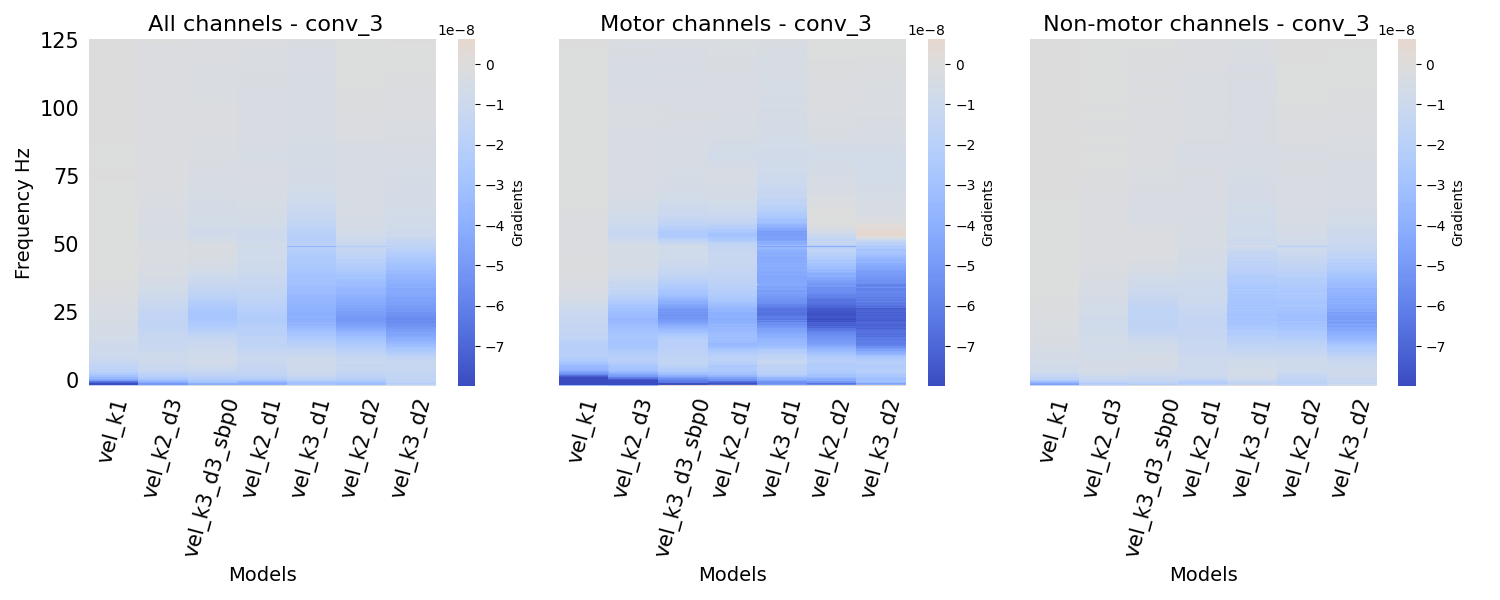
\includegraphics[width=0.85\linewidth]{img/appendix/A/conv-3/sm/vel-model-gradients-all_kinds}
   \caption{}
   \label{fig:vel-shifted-grads-conv-3}
\end{subfigure}
\end{figure}
\clearpage   

\begin{figure}[!htbp]\ContinuedFloat

\begin{subfigure}[b]{\textwidth}
   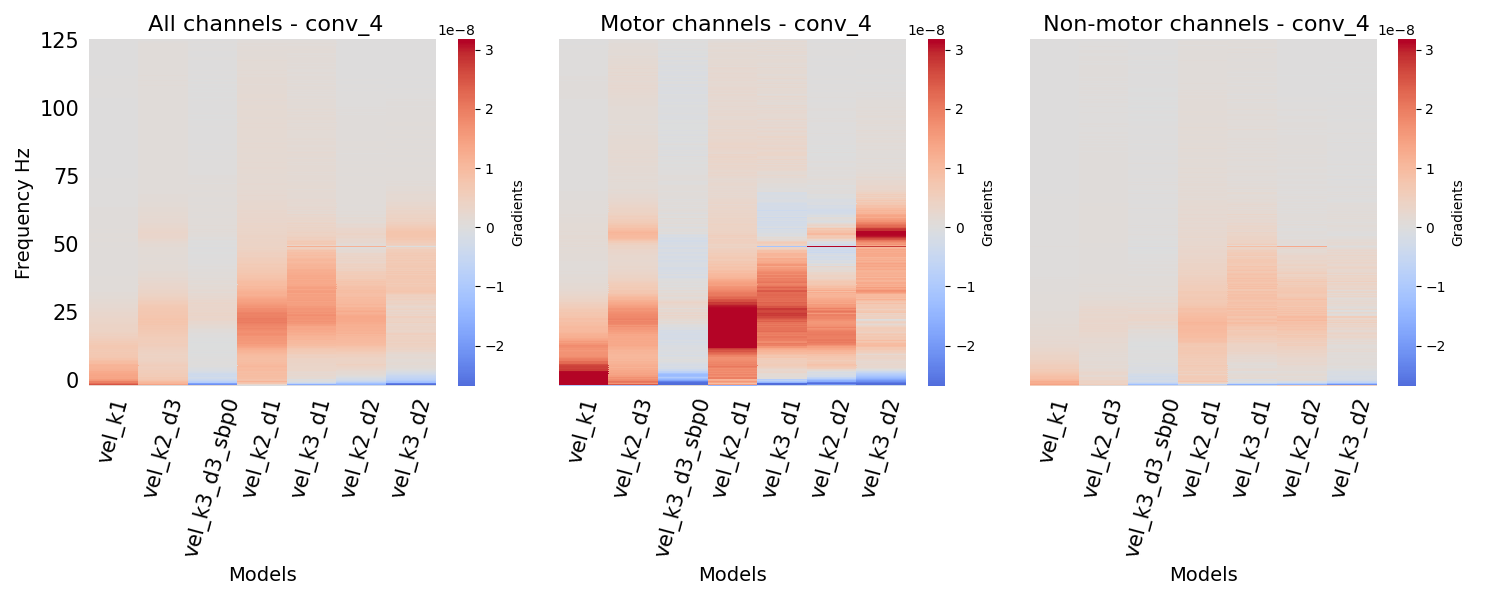
\includegraphics[width=1\linewidth]{img/appendix/A/conv-4/sm/vel-model-gradients_all_kinds}
   \caption{}
   \label{fig:vel-shifted-grads-conv-4}
\end{subfigure}

\begin{subfigure}[b]{\textwidth}
   \includegraphics[width=1\linewidth]{img/appendix/A/conv-classifier/sm/vel-model-gradients_all_kinds}
   \caption{}
   \label{fig:vel-shifted-grads-conv-classifier}
\end{subfigure}

\caption[]{Gradients of the different CNN architectures decoding velocity from the full dataset in the shifted setting (acausal prediction) (see Section~\ref{subsec:shifting-the-predicted-time-point-to-the-centre-of-the-receptive-field}. \textbf{(a)} shows gradients of the convolutional layer in the second block; \textbf{(b)} shows gradients of the convolutional layer in the third block; \textbf{(c)} shows gradients of the fourth convolutional block; \textbf{(d)} shows gradients of the last convolutional layer - the output layer. All channels include channels that do not belong to motor neither non-motor channel sets. See Section \ref{subsec:ieeg-data-preprocessing}}
\label{fig:vel-shifted-grads}
\end{figure}
\clearpage
\section*{Velocity - High-passed dataset}\label{subsec:vel-high-passed-dataset-appendixB}
\begin{figure}[!htpb]
\centering
\begin{subfigure}[b]{\textwidth}
   \includegraphics[width=1\linewidth]{img/appendix/A/conv-2/hp-sm/vel-model-gradients_all_kinds}
   \caption{}
   \label{fig:vel-hp-shifted-grads-conv-2}
\end{subfigure}

\begin{subfigure}[b]{\textwidth}
   \includegraphics[width=1\linewidth]{img/appendix/A/conv-3/hp-sm/vel-model-gradients_all_kinds}
   \caption{}
   \label{fig:vel-hp-shifted-grads-conv-3}
\end{subfigure}

\end{figure}
\clearpage   

\begin{figure}[!htbp]\ContinuedFloat
\begin{subfigure}[b]{\textwidth}
   \includegraphics[width=1\linewidth]{img/appendix/A/conv-4/hp-sm/vel-model_gradients_all_kinds}
   \caption{}
   \label{fig:vel-hp-shifted-grads-conv-4}
\end{subfigure}

\begin{subfigure}[b]{\textwidth}
   \includegraphics[width=1\linewidth]{img/appendix/A/conv-classifier/hp-sm/vel-model_gradients_all_kinds}
   \caption{}
   \label{fig:vel-hp-shifted-grads-conv-classifier}
\end{subfigure}

\caption[]{Gradients of the different CNN architectures decoding velocity from the high-passed dataset in the shifted setting (acausal prediction) (see Section~\ref{subsec:shifting-the-predicted-time-point-to-the-centre-of-the-receptive-field}. \textbf{(a)} shows gradients of the convolutional layer in the second block; \textbf{(b)} shows gradients of the convolutional layer in the third block; \textbf{(c)} shows gradients of the fourth convolutional block; \textbf{(d)} shows gradients of the last convolutional layer - the output layer. All channels include channels that do not belong to motor neither non-motor channel sets. See Section \ref{subsec:ieeg-data-preprocessing}}
\label{fig:vel-hp-shifted-grads}
\end{figure}

\clearpage
\section*{Absolute velocity - Full dataset}\label{sec:absolute-velocity-appendixB}

\begin{figure}[!htpb]
\centering
\begin{subfigure}[b]{\textwidth}
   \includegraphics[width=1\linewidth]{img/appendix/A/conv-2/sm/absVel-model-gradients-all_kinds}
   \caption{}
   \label{fig:absVel-shifted-grads-conv-2}
\end{subfigure}

\begin{subfigure}[b]{\textwidth}
   \includegraphics[width=1\linewidth]{img/appendix/A/conv-3/sm/absVel-model-gradients-all_kinds}
   \caption{}
   \label{fig:absVel-shifted-grads-conv-3}
\end{subfigure}
\end{figure}
\clearpage   

\begin{figure}[!htbp]\ContinuedFloat
\begin{subfigure}[b]{\textwidth}
   \includegraphics[width=1\linewidth]{img/appendix/A/conv-4/sm/absVel-model-gradients_all_kinds}
   \caption{}
   \label{fig:absVel-shifted-grads-conv-4}
\end{subfigure}

\begin{subfigure}[b]{\textwidth}
   \includegraphics[width=1\linewidth]{img/appendix/A/conv-classifier/sm/absVel-model-gradients_all_kinds}
   \caption{}
   \label{fig:absVel-shifted-grads-conv-classifier}
\end{subfigure}

\caption[]{Gradients of the different CNN architectures decoding absolute velocity from the full dataset in the shifted setting (acausal prediction) (see Section~\ref{subsec:shifting-the-predicted-time-point-to-the-centre-of-the-receptive-field}. \textbf{(a)} shows gradients of the convolutional layer in the second block; \textbf{(b)} shows gradients of the convolutional layer in the third block; \textbf{(c)} shows gradients of the fourth convolutional block; \textbf{(d)} shows gradients of the last convolutional layer - the output layer. All channels include channels that do not belong to motor neither non-motor channel sets. See Section \ref{subsec:ieeg-data-preprocessing}}
\label{fig:absVel-shifted-grads}
\end{figure}

\clearpage
\section*{Absolute velocity - High-passed dataset}\label{subsec:absVel-high-passed-dataset-appendixB}
\begin{figure}[!htpb]
\centering
\begin{subfigure}[b]{\textwidth}
   \includegraphics[width=1\linewidth]{img/appendix/A/conv-2/hp-sm/absVel-model-gradients_all_kinds}
   \caption{}
   \label{fig:absVel-hp-shifted-grads-conv-2}
\end{subfigure}

\begin{subfigure}[b]{\textwidth}
   \includegraphics[width=1\linewidth]{img/appendix/A/conv-3/hp-sm/absVel-model-gradients_all_kinds}
   \caption{}
   \label{fig:absVel-hp-shifted-grads-conv-3}
\end{subfigure}
\end{figure}
\clearpage   

\begin{figure}[!htbp]\ContinuedFloat
\begin{subfigure}[b]{\textwidth}
   \includegraphics[width=1\linewidth]{img/appendix/A/conv-4/hp-sm/absVel-model_gradients_all_kinds}
   \caption{}
   \label{fig:absVel-hp-shifted-grads-conv-4}
\end{subfigure}

\begin{subfigure}[b]{\textwidth}
   \includegraphics[width=1\linewidth]{img/appendix/A/conv-classifier/hp-sm/absVel-model_gradients_all_kinds}
   \caption{}
   \label{fig:absVel-hp-shifted-grads-conv-classifier}
\end{subfigure}

\caption[]{Gradients of the different CNN architectures decoding absolute velocity from the high-passed dataset in the shifted setting (acausal prediction) (see Section~\ref{subsec:shifting-the-predicted-time-point-to-the-centre-of-the-receptive-field}. \textbf{(a)} shows gradients of the convolutional layer in the second block; \textbf{(b)} shows gradients of the convolutional layer in the third block; \textbf{(c)} shows gradients of the fourth convolutional block; \textbf{(d)} shows gradients of the last convolutional layer - the output layer. All channels include channels that do not belong to motor neither non-motor channel sets. See Section \ref{subsec:ieeg-data-preprocessing}}
\label{fig:absVel-hp-shifted-grads}
\end{figure}
\chapter{Gradients of all architectures - gradually shifted}\label{appendixC}

\section*{Velocity - Full dataset}\label{sec:velocity-appendixC}

\begin{figure}[!htpb]
\centering
\begin{subfigure}[b]{\textwidth}
   \includegraphics[width=1\linewidth]{img/appendix/C/m/vel/sbp0_m_shift_gradients_conv_2_all_kinds}
   \caption{}
   \label{fig:vel-shifting-grads-conv-2}
\end{subfigure}

\begin{subfigure}[b]{\textwidth}
   \includegraphics[width=1\linewidth]{img/appendix/C/m/vel/sbp0_m_shift_gradients_conv_3_all_kinds}
   \caption{}
   \label{fig:vel-shifting-grads-conv-3}
\end{subfigure}
\end{figure}
\clearpage
\begin{figure}
\ContinuedFloat

\begin{subfigure}[b]{\textwidth}
   \includegraphics[width=1\linewidth]{img/appendix/C/m/vel/sbp0_m_shift_gradients_conv_4_all_kinds}
   \caption{}
   \label{fig:vel-shifting-grads-conv-4}
\end{subfigure}

\begin{subfigure}[b]{\textwidth}
   \includegraphics[width=1\linewidth]{img/appendix/C/m/vel/sbp0_m_shift_gradients_conv_classifier_all_kinds}
   \caption{}
   \label{fig:vel-shifting-grads-conv-classifier}
\end{subfigure}

\caption[]{Gradients of the different CNN architectures decoding velocity from the full dataset when gradually shifting the predicted time-point (see Section~\ref{subsec:shifting-the-predicted-time-point-across-receptive-field}. \textbf{(a)} shows gradients of the convolutional layer in the second block; \textbf{(b)} shows gradients of the convolutional layer in the third block; \textbf{(c)} shows gradients of the fourth convolutional block; \textbf{(d)} shows gradients of the last convolutional layer - the output layer. All channels include channels that do not belong to motor neither non-motor channel sets. See Section \ref{subsec:ieeg-data-preprocessing}}
\label{fig:vel-shifting-grads}
\end{figure}

\clearpage
\section*{Velocity - High-passed dataset}\label{subsec:vel-high-passed-dataset-appendixC}
\begin{figure}[!htpb]
\centering
\begin{subfigure}[b]{\textwidth}
   \includegraphics[width=0.85\linewidth]{img/appendix/C/hp-m/vel/sbp0_hp_m_shift_gradients_conv_2_all_kinds}
   \caption{}
   \label{fig:vel-hp-shifting-grads-conv-2}
\end{subfigure}

\begin{subfigure}[b]{\textwidth}
   \includegraphics[width=0.85\linewidth]{img/appendix/C/hp-m/vel/sbp0_hp_m_shift_gradients_conv_3_all_kinds}
   \caption{}
   \label{fig:vel-hp-shifting-grads-conv-3}
\end{subfigure}

\begin{subfigure}[b]{\textwidth}
   \includegraphics[width=0.85\linewidth]{img/appendix/C/hp-m/vel/sbp0_hp_m_shift_gradients_conv_4_all_kinds}
   \caption{}
   \label{fig:vel-hp-shifting-grads-conv-4}
\end{subfigure}

\begin{subfigure}[b]{\textwidth}
   \includegraphics[width=0.85\linewidth]{img/appendix/C/hp-m/vel/sbp0_hp_m_shift_gradients_conv_classifier_all_kinds}
   \caption{}
   \label{fig:vel-hp-shifting-grads-conv-classifier}
\end{subfigure}

\caption[]{Gradients of the different CNN architectures decoding velocity from the high-passed dataset when gradually shifting the predicted time-point (see Section~\ref{subsec:shifting-the-predicted-time-point-across-receptive-field}. \textbf{(a)} shows gradients of the convolutional layer in the second block; \textbf{(b)} shows gradients of the convolutional layer in the third block; \textbf{(c)} shows gradients of the fourth convolutional block; \textbf{(d)} shows gradients of the last convolutional layer - the output layer. All channels include channels that do not belong to motor neither non-motor channel sets. See Section \ref{subsec:ieeg-data-preprocessing}}
\label{fig:vel-hp-shifting-grads}
\end{figure}
\clearpage
\section*{Absolute velocity - Full dataset}\label{sec:absolute-velocity-appendixC}

\begin{figure}[!htpb]
\centering
\begin{subfigure}[b]{\textwidth}
   \includegraphics[width=0.85\linewidth]{img/appendix/C/m/absVel/sbp0_m_shift_gradients_conv_2_all_kinds}
   \caption{}
   \label{fig:absVel-shifting-grads-conv-2}
\end{subfigure}

\begin{subfigure}[b]{\textwidth}
   \includegraphics[width=0.85\linewidth]{img/appendix/C/m/absVel/sbp0_m_shift_gradients_conv_3_all_kinds}
   \caption{}
   \label{fig:absVel-shifting-grads-conv-3}
\end{subfigure}

\begin{subfigure}[b]{\textwidth}
   \includegraphics[width=0.85\linewidth]{img/appendix/C/m/absVel/sbp0_m_shift_gradients_conv_4_all_kinds}
   \caption{}
   \label{fig:absVel-shifting-grads-conv-4}
\end{subfigure}

\begin{subfigure}[b]{\textwidth}
   \includegraphics[width=0.85\linewidth]{img/appendix/C/m/absVel/sbp0_m_shift_gradients_conv_classifier_all_kinds}
   \caption{}
   \label{fig:absVel-shifting-grads-conv-classifier}
\end{subfigure}

\caption[]{Gradients of the different CNN architectures decoding absolute velocity from the full dataset when gradually shifting the predicted time-point (see Section~\ref{subsec:shifting-the-predicted-time-point-across-receptive-field}. \textbf{(a)} shows gradients of the convolutional layer in the second block; \textbf{(b)} shows gradients of the convolutional layer in the third block; \textbf{(c)} shows gradients of the fourth convolutional block; \textbf{(d)} shows gradients of the last convolutional layer - the output layer. All channels include channels that do not belong to motor neither non-motor channel sets. See Section \ref{subsec:ieeg-data-preprocessing}}
\label{fig:absVel-shifting-grads}
\end{figure}

\clearpage
\section*{Absolute velocity - High-passed dataset}\label{subsec:absVel-high-passed-dataset-appendixC}
\begin{figure}[!htpb]
\centering
\begin{subfigure}[b]{\textwidth}
   \includegraphics[width=0.85\linewidth]{img/appendix/C/hp-m/absVel/sbp0_hp_m_shift_gradients_conv_2_all_kinds}
   \caption{}
   \label{fig:absVel-hp-shifting-grads-conv-2}
\end{subfigure}

\begin{subfigure}[b]{\textwidth}
   \includegraphics[width=0.85\linewidth]{img/appendix/C/hp-m/absVel/sbp0_hp_m_shift_gradients_conv_3_all_kinds}
   \caption{}
   \label{fig:absVel-hp-shifting-grads-conv-3}
\end{subfigure}

\begin{subfigure}[b]{\textwidth}
   \includegraphics[width=0.85\linewidth]{img/appendix/C/hp-m/absVel/sbp0_hp_m_shift_gradients_conv_4_all_kinds}
   \caption{}
   \label{fig:absVel-hp-shifting-grads-conv-4}
\end{subfigure}

\begin{subfigure}[b]{\textwidth}
   \includegraphics[width=0.85\linewidth]{img/appendix/C/hp-m/absVel/sbp0_hp_m_shift_gradients_conv_classifier_all_kinds}
   \caption{}
   \label{fig:absVel-hp-shifting-grads-conv-classifier}
\end{subfigure}

\caption[]{Gradients of the different CNN architectures decoding absolute velocity from the high-passed dataset when gradually shifting the predicted time-point (see Section~\ref{subsec:shifting-the-predicted-time-point-across-receptive-field}. \textbf{(a)} shows gradients of the convolutional layer in the second block; \textbf{(b)} shows gradients of the convolutional layer in the third block; \textbf{(c)} shows gradients of the fourth convolutional block; \textbf{(d)} shows gradients of the last convolutional layer - the output layer. All channels include channels that do not belong to motor neither non-motor channel sets. See Section \ref{subsec:ieeg-data-preprocessing}}
\label{fig:absVel-hp-shifting-grads}
\end{figure}
\chapter{Gradients of all architectures - spectral whitening}\label{appendixD}

\section*{Velocity - Full dataset}\label{sec:velocity-appendixD}

\begin{figure}[!htpb]
\centering
\begin{subfigure}[b]{\textwidth}
   \includegraphics[width=0.85\linewidth]{img/appendix/D/conv-2/m/vel_model_gradients_all_kinds}
   \caption{}
   \label{fig:vel-pw-full-grads-conv-2}
\end{subfigure}

\begin{subfigure}[b]{\textwidth}
   \includegraphics[width=0.85\linewidth]{img/appendix/D/conv-3/m/vel_model_gradients_all_kinds}
   \caption{}
   \label{fig:vel-pw-full-grads-conv-3}
\end{subfigure}
\end{figure}
\clearpage   

\begin{figure}[!htbp]\ContinuedFloat

\begin{subfigure}[b]{\textwidth}
   \includegraphics[width=0.85\linewidth]{img/appendix/D/conv-4/m/vel_model_gradients_all_kinds}
   \caption{}
   \label{fig:vel-pw-full-grads-conv-4}
\end{subfigure}

\begin{subfigure}[b]{\textwidth}
   \includegraphics[width=0.85\linewidth]{img/appendix/D/conv-classifier/m/vel_model_gradients_all_kinds}
   \caption{}
   \label{fig:vel-pw-full-grads-conv-classifier}
\end{subfigure}

\caption[]{Gradients of the different CNN architectures decoding velocity from the full whitened dataset in the original non-shifted setting (causal prediction) (see Section~\ref{sec:spectral-whitening}). \textbf{(a)} shows gradients of the convolutional layer in the second block; \textbf{(b)} shows gradients of the convolutional layer in the third block; \textbf{(c)} shows gradients of the fourth convolutional block; \textbf{(d)} shows gradients of the last convolutional layer - the output layer. All channels include channels that do not belong to motor neither non-motor channel sets. See Section \ref{subsec:ieeg-data-preprocessing}}
\label{fig:vel-pw-full-grads}
\end{figure}

\clearpage
\section*{Absolute velocity - High-passed dataset}\label{subsec:vel-high-passed-dataset-appendixD}
\begin{figure}[!htpb]
\centering
\begin{subfigure}[b]{\textwidth}
   \includegraphics[width=1\linewidth]{img/appendix/D/conv-2/hp-sm/vel_model_gradients_all_kinds}
   \caption{}
   \label{fig:vel-pw-hp-grads-conv-2}
\end{subfigure}

\begin{subfigure}[b]{\textwidth}
   \includegraphics[width=1\linewidth]{img/appendix/D/conv-3/hp-m/vel_model_gradients_all_kinds}
   \caption{}
   \label{fig:vel-pw-hp-grads-conv-3}
\end{subfigure}
\end{figure}
\clearpage   

\begin{figure}[!htbp]\ContinuedFloat

\begin{subfigure}[b]{\textwidth}
   \includegraphics[width=1\linewidth]{img/appendix/D/conv-4/hp-m/vel_model_gradients_all_kinds}
   \caption{}
   \label{fig:vel-pw-hp-grads-conv-4}
\end{subfigure}


\begin{subfigure}[b]{\textwidth}
   \includegraphics[width=1\linewidth]{img/appendix/D/conv-classifier/hp-m/vel_model_gradients_all_kinds}
   \caption{}
   \label{fig:vel-pw-hp-grads-conv-classifier}
\end{subfigure}

\caption[]{Gradients of the different CNN architectures decoding velocity from the high-passed, whitened dataset in the original non-shifted setting (causal prediction) (see Section~\ref{sec:spectral-whitening}). \textbf{(a)} shows gradients of the convolutional layer in the second block; \textbf{(b)} shows gradients of the convolutional layer in the third block; \textbf{(c)} shows gradients of the fourth convolutional block; \textbf{(d)} shows gradients of the last convolutional layer - the output layer. All channels include channels that do not belong to motor neither non-motor channel sets. See Section \ref{subsec:ieeg-data-preprocessing}}
\label{fig:vel-pw-hp-grads}
\end{figure}

\clearpage
\section*{Absolute velocity - Full dataset}\label{sec:absolute-velocity-appendixD}
\begin{figure}[!htpb]
\centering
\begin{subfigure}[b]{\textwidth}
   \includegraphics[width=1\linewidth]{img/appendix/D/conv-2/m/absVel_model_gradients_all_kinds}
   \caption{}
   \label{fig:absVel-pw-full-grads-conv-2}
\end{subfigure}

\begin{subfigure}[b]{\textwidth}
   \includegraphics[width=1\linewidth]{img/appendix/D/conv-3/m/absVel_model_gradients_all_kinds}
   \caption{}
   \label{fig:absVel-pw-full-grads-conv-3}
\end{subfigure}
\end{figure}
\clearpage   

\begin{figure}[!htbp]\ContinuedFloat

\begin{subfigure}[b]{\textwidth}
   \includegraphics[width=1\linewidth]{img/appendix/D/conv-4/m/absVel_model_gradients_all_kinds}
   \caption{}
   \label{fig:absVel-pw-full-grads-conv-4}
\end{subfigure}

\begin{subfigure}[b]{\textwidth}
   \includegraphics[width=1\linewidth]{img/appendix/D/conv-classifier/m/absVel_model_gradients_all_kinds}
   \caption{}
   \label{fig:absVel-pw-full-grads-conv-classifier}
\end{subfigure}

\caption[]{Gradients of the different CNN architectures decoding absolute velocity from the full whitened dataset in the original non-shifted setting (causal prediction) (see Section~\ref{sec:spectral-whitening}). \textbf{(a)} shows gradients of the convolutional layer in the second block; \textbf{(b)} shows gradients of the convolutional layer in the third block; \textbf{(c)} shows gradients of the fourth convolutional block; \textbf{(d)} shows gradients of the last convolutional layer - the output layer. All channels include channels that do not belong to motor neither non-motor channel sets. See Section \ref{subsec:ieeg-data-preprocessing}}
\label{fig:absVel-pw-full-grads}
\end{figure}

\clearpage
\section*{Absolute velocity - High-passed dataset}\label{subsec:absVel-high-passed-dataset-appendixD}
\begin{figure}[!htpb]
\centering
\begin{subfigure}[b]{\textwidth}
   \includegraphics[width=1\linewidth]{img/appendix/D/conv-2/hp-m/absVel_model_gradients_all_kinds}
   \caption{}
   \label{fig:absVel-pw-hp-grads-conv-2}
\end{subfigure}

\begin{subfigure}[b]{\textwidth}
   \includegraphics[width=1\linewidth]{img/appendix/D/conv-3/hp-m/absVel_model_gradients_all_kinds}
   \caption{}
   \label{fig:absVel-pw-hp-grads-conv-3}
\end{subfigure}
\end{figure}
\clearpage   

\begin{figure}[!htbp]\ContinuedFloat
\begin{subfigure}[b]{\textwidth}
   \includegraphics[width=1\linewidth]{img/appendix/D/conv-4/hp-m/absVel_model_gradients_all_kinds}
   \caption{}
   \label{fig:absVel-pw-hp-grads-conv-4}
\end{subfigure}

\begin{subfigure}[b]{\textwidth}
   \includegraphics[width=1\linewidth]{img/appendix/D/conv-classifier/hp-m/absVel_model_gradients_all_kinds}
   \caption{}
   \label{fig:absVel-pw-hp-grads-conv-classifier}
\end{subfigure}

\caption[]{Gradients of the different CNN architectures decoding absolute velocity from the high-passed whitened dataset in the original non-shifted setting (causal prediction) (see Section~\ref{sec:spectral-whitening}). \textbf{(a)} shows gradients of the convolutional layer in the second block; \textbf{(b)} shows gradients of the convolutional layer in the third block; \textbf{(c)} shows gradients of the fourth convolutional block; \textbf{(d)} shows gradients of the last convolutional layer - the output layer. All channels include channels that do not belong to motor neither non-motor channel sets. See Section \ref{subsec:ieeg-data-preprocessing}}
\label{fig:absVel-pw-hp-grads}
\end{figure}

% if your attachments are complicated, describe them in a separate appendix
%\include{attachments}

\openright
\end{document}
